\documentclass[11pt]{book}
\title{\textbf{Citogenetica e Ingegneria Cromosomica}}
\author{Simona Debilio}
\date{A.A. 2018/2019}
% manually added packages
\usepackage[margin=1in]{geometry}
\usepackage[italian]{babel}
% ====================================================
\usepackage{lmodern}
\usepackage{amssymb,amsmath}
\usepackage{ifxetex,ifluatex}
\usepackage{fixltx2e} % provides \textsubscript
\ifnum 0\ifxetex 1\fi\ifluatex 1\fi=0 % if pdftex
  \usepackage[T1]{fontenc}
  \usepackage[utf8]{inputenc}
\else % if luatex or xelatex
  \ifxetex
    \usepackage{mathspec}
    \usepackage{xltxtra,xunicode}
  \else
    \usepackage{fontspec}
  \fi
  \defaultfontfeatures{Mapping=tex-text,Scale=MatchLowercase}
  \newcommand{\euro}{€}
\fi
% use upquote if available, for straight quotes in verbatim environments
\IfFileExists{upquote.sty}{\usepackage{upquote}}{}
% use microtype if available
\IfFileExists{microtype.sty}{%
\usepackage{microtype}
\UseMicrotypeSet[protrusion]{basicmath} % disable protrusion for tt fonts
}{}
\ifxetex
  \usepackage[setpagesize=false, % page size defined by xetex
              unicode=false, % unicode breaks when used with xetex
              xetex]{hyperref}
\else
  \usepackage[unicode=true]{hyperref}
\fi
\hypersetup{breaklinks=true,
            bookmarks=true,
            pdfauthor={},
            pdftitle={},
            colorlinks=true,
            citecolor=blue,
            urlcolor=blue,
            linkcolor=magenta,
            pdfborder={0 0 0}}
\urlstyle{same}  % don't use monospace font for urls
\setlength{\parindent}{0pt}
\setlength{\parskip}{6pt plus 2pt minus 1pt}
\setlength{\emergencystretch}{3em}  % prevent overfull lines
\setcounter{secnumdepth}{0}

\date{}

\setlength{\parindent}{0pt}

\usepackage{graphicx}
\usepackage{caption}
\usepackage{subcaption}
\usepackage{siunitx}
\usepackage{wrapfig}

\begin{document}

\maketitle

\tableofcontents

\chapter{Programma}

Il programma delle lezioni prevede:

\begin{itemize}
\item 
Cenni storici;
\item 
Citogenetica classica e nuova;
\item 
Condensazione del DNA nel cromosoma eucariotico:

	\begin{enumerate}
	\item strutture ad anse e ruolo regolativo;
	\end{enumerate}

\item 
Metodi di localizzazione genica:

	\begin{enumerate}
	\item
	Ibridazione di cellule somatiche;
	\item 
	Ibridazione in situ;
	\end{enumerate}

\item 
Regolazione dell’espressione genica negli eucarioti multicellulari:

	\begin{enumerate}
	\item 
	Puffering (cromosomi politenici);
    \item 
    Trascrizione rDNA (cromosomi a spazzola);
    \item
    Determinazione del sesso;
    \item
    Compensazione del dosaggio nei mammiferi;
    \item
    Compensazione del dosaggio in Drosophila;
    \end{enumerate}

\item 
Imprinting genomico;
\item
Struttura del genoma degli eucarioti:

	\begin{enumerate}
    \item
    Progetti genoma;
    \item 
    Sequenze uniche e ripetute;
    \item
    Non coding RNA;
    \end{enumerate}
    
\item 
Citogenetica dei tumori:

	\begin{enumerate}
	\item
	Generalità;
    \item
    Esempi specifici: linfoma di Burkitt, LMC ph+, Retinoblastoma;
    \end{enumerate}
    
\item
Instabilità genomica:

	\begin{enumerate}
	\item
    Duplicazioni segmentali;
    \item
    Disordini genomici;
    \item
    Duplicazioni segmentali;
    \end{enumerate}
    
\item
Elementi funzionali del cromosoma eucariotico:

	\begin{enumerate}
    \item
    Telomeri;
    \item
    Origini di replicazione;
    \item
    Centromeri:
    \end{enumerate}
    	
		\begin{itemize}
        \item
        DNA centromerico;
        \item
        Proteine centromeriche;
        \item
        Paradosso del centromero;
        \item
        I centromeri nell’evoluzione;
        \end{itemize}
        
\item
Ricostruzione del cromosoma:
	
	\begin{enumerate}
    \item
    Cromosomi artificiali;
    \item
    Vettori cromosomici;
    \item
    Cromosomi artificiali di mammifero;
    \item
    Metodo bottom-up;
    \item
    Metodo bottom-down
    \end{enumerate}

\item
Terapia genica:

	\begin{enumerate}
    \item
    Terapia genica germinale;
    \item
    Terapia genica somatica;
    \item
    Terapia genica nei tumori;
    \item
    Problemi etici;
    \end{enumerate}

\item
Cellule staminali:

	\begin{enumerate}
    \item
    cellule staminali embrionali;
    \item
    cellule embrionali fetali e adulte;
    \item
    cellule iPS (inuced Pluripotent Stem Cells);
    \end{enumerate}
    
\item
Clonazione:

	\begin{enumerate}
    \item
    clonazione vegetale;
    \item
    conazione animale;
    \item
    clonazione terapeutica;
    \item
    clonazione riproduttiva;
    \item
    problemi etici.
    \end{enumerate}
\end{itemize}

\chapter{Introduzione}

La condensazione del DNA nel cromosoma eucariotico presenta un ruolo regolativo importante e rappresenta la base della regolazione epigenetica dell’espressione genica.

I cromosomi politenici di Drosophila sono, ad oggi, protagonisti della genetica molecolare. Drosophila continua infatti ad essere un ottimo modello per lo studio degli eucarioti poiché:
\begin{itemize}
\item
il numero di marcatori conosciuti è elevato;
\item
consente di seguire i diversi stadi di sviluppo;
\item
è un modello trasferibile negli eucarioti superiori.
\end{itemize} 

Un cromosoma politenico è un cromosoma gigante. I cromosomi politenici si formano in seguito a vari cicli di replicazione che producono molte copie (anche centinaia) di cromatidi fratelli che rimangono uniti.
La formazione dei cromosomi politenici ha la funzione di aumentare il volume cellulare ma può anche comportare un vantaggio metabolico dato che l'elevato numero di copie di geni permette un alto livello di espressione genica. In Drosophila melanogaster, per esempio, i cromosomi delle ghiandole salivari delle larve subiscono numerosi cicli di endoreplicazione, e questo consente di produrre grandi quantità di secreto prima dell'impupamento.
Al microscopio i cromosomi politenici mostrano caratteristici pattern di bande chiare e scure che possono essere utilizzati per identificare riarrangiamenti cromosomici e delezioni. Bande scure corrispondono spesso alla cromatina inattiva, mentre bande chiare si trovano di solito in aree con una maggiore attività trascrizionale.

La citogenetica è una branca della genetica. Il termine \emph{citogenetica} significa ``studio dei cromosomi'', si tratta quindi di una disciplina confinata alla descrizione dei cromosomi basata sull’utilizzo del microscopio.
In realtà oggi la citogenetica è descritta in maniera differente poiché, nel tempo, si è adeguata alle esigenze della biologia molecolare diventando strettamente complementare alle nuove tecnologie, note come post-genomica, che hanno raggiunto delle capacità descrittive, risolutive, e funzionali elevate; la citogenetica risulta quindi essere complementare alla genomica-post genomica. 

L’\emph{ingegneria cromosomica} rappresenta, invece, lo studio molecolare dei cromosomi utile per la costruzione di cromosomi artificiali.  

\section{Citogenetica classica e nuova citogenetica}
La citogenetica classica è una disciplina più vecchia della genetica, che nasce con la scoperta del microscopio e che su di esso si basa. Già i primi microscopisti, analizzando gli apici radicali delle piante e alcuni tessuti di organismi molto semplici, videro che vi erano delle cellule che subivano dei cicli di divisione cellulare e descrissero dettagliatamente i processi di meiosi e mitosi, prima ancora che nascesse la genetica.

La \textbf{citogenetica classica} consiste nello studio morfologico, al microscopio, del comportamento dei cromosomi alla mitosi e alla meiosi. 
Già i primi microscopisti si resero conto del fatto che vi fosse una grossa differenza tra ciò che avveniva nelle cellule mitotiche e in quelle meiotiche; essi infatti descrissero la segregazione dei cromosomi con una distribuzione equivalente del materiale genetico nelle cellule figlie durante la mitosi e scoprirono, invece, che vi erano alcuni tessuti in cui avveniva un dimezzamento del numero cromosomico a seguito della formazione dei gameti. Quanto scoperto a quei tempi risultò essere di difficile comprensione, ma risultò poi essere molto chiaro nel momento in cui la citogenetica e la genetica mendeliana si unirono in un’unica cosa che permise di capire che il comportamento dei cromosomi spiegava l’eredità mendeliana.

La citogenetica ha avuto una grossa spinta grazie all’evoluzione delle nuove tecnologie in campo umano, infatti già alla fine degli anni '50 questa disciplina risultò essere fondamentale per l’analisi del cariotipo umano normale e patologico, cioè per capire quali fossero le basi cromosomiche di alcune patologie e per la diagnosi delle stesse.

Fondamentali per poter identificare i cromosomi sono le tecniche di colorazione differenziale e le colture in vitro di cellule somatiche (i cromosomi risultano essere visibili durante la divisione cellulare). Se per i primi microscopisti lo studio dei tessuti meristematici degli apici radicali, trattandosi di tessuti in continua rigenerazione, non risultò essere difficile, lo studio dei cromosomi durante la divisione cellulare risultò invece più arduo a causa della difficoltà nel ritrovare tessuti in attiva rigenerazione spontanea nell’uomo. Tessuti di questo tipo ve ne sono, ma risultano essere difficilmente raggiungibili con tecniche non invasive (es. midollo osseo, tessuti tumorali e tessuti germinali).
Per questo motivo sono state sviluppate delle tecniche in grado di stimolare la proliferazione di tessuti differenziati che normalmente non si dividerebbero. Il tessuto di elezione è rappresentato dal sangue periferico, è infatti possibile indurre le cellule nucleate (linfociti) a proliferare; lo stesso può essere fatto effettuando dei piccoli espianti cutanei prelevando qualche mm\(^2\) di tessuto sottocutaneo.

La citogenetica classica è stata, fondamentalmente, la base delle leggi di Mendel. In passato vi fu un momento in cui la citogenetica classica, con l’avvento della biologia molecolare, sembrava fosse divenuta incapace di descrivere dettagli, soprattutto funzionali, che invece la biologia molecolare poteva arrivare a definire; veniva infatti considerata una ``cenerentola o un’ancella povera'' come quasi tutte le discipline morfologico-descrittive.
In realtà vi fu un’evoluzione sempre più veloce tale per cui la nuova citogenetica rappresenta sempre lo studio dei cromosomi ma con delle tecniche ad altissima risoluzione, fino ad arrivare a livelli di risoluzione comparabili a quelli della biologia molecolare delle analisi di sequenza.
La nuova citogenetica è quindi, a tutt’oggi, la base fisica della genetica, della biologia molecolare e della biologia strutturale perché permette di descrivere l’anatomia molecolare del cromosoma arrivando, addirittura, a ricostruirlo. 

Dal momento che la citogenetica possiede una visione d’insieme, risulterà essere molto importante perché rappresenterà il punto di partenza e di arrivo per l’analisi dei genomi complessi. Infatti, una volta stabiliti dei dettagli molecolari è importante poterli inserire in un contesto cromatinico definito, sarà proprio in questa fase che risulterà essere fondamentale la citogenetica.
Oggi è possibile fare una citogenetica di nuova generazione, basata sull’uso della citogenetica in assenza dei cromosomi e nota come citogenomica.

La patologia costituzionale e la citogenetica oncologica trovano un supporto insostituibile nello sviluppo di tecniche ad alta risoluzione che ad oggi permettono di fare delle descrizioni dettagliate delle diverse anomalie associate al cancro. Con la citogenetica è possibile stabilire, a livello molecolare, i punti di rottura coinvolti nei ri-arrangiamenti e, quindi, delimitare delle regioni critiche all’interno delle quali cercare oncogeni o oncosoppressori coinvolti nello sviluppo di quel particolare tipo di tumore; ciò risulterà avere un’importanza diagnostica e pronostica.

\section{Il cromosoma}
Il termina cromosoma è stato introdotto nel 1888 da Wilhelm Waldeier e classicamente risulta essere definito come \emph{un ``corpo colorato'' evidenziabile con coloranti basici durante la divisione cellulare} (mitosi, meiosi).

In realtà, ad oggi, la definizione appena data risulta essere superata poiché è definibile come cromosoma \emph{una qualsiasi molecola di acido nucleico che contenga l’informazione per la sintesi di tutte le proteine di un certo organismo, dotata di replicazione autonoma (origini di replicazione), circolare o lineare (nel secondo caso dotata di telomeri) e in grado di segregare fedelmente nelle cellule figlie (funzione espletata dal centromero).}

Il cromosoma eucariotico, durante la metafase, è costituito da due cromatidi fratelli (identici) legati al centromero. Ogni cromatidio è una molecola di DNA lineare e la ricombinazione tra cromatidi fratelli non determina un ri-arrangiamento cromosomico, ma solamente uno scambio di elementi.\\
In ogni eucariote diploide ogni cromosoma è presente in due copie, uno di origine materna e uno di origine paterna, tra loro omologhi. Gli omologhi non sono identici ma possono differire per varianti alleliche a tutti i loci.
Quanto appena detto risulterà essere particolarmente importante poiché rappresentante la base della replicazione sessuata e, quindi, la base della variabilità degli organismi.  

Il microscopio elettronico non aggiunge dettagli alla struttura del cromosoma poiché lo mostra semplicemente più grande e rappresentato da un caotico super-avvolgimento di una fibra non meglio identificata.\\
Il cromosoma eucariotico è formato da un braccio corto (\emph{p}, petit - la prima conferenza per la standardizzazione della nomenclatura citogenetica si svolse in Francia) e uno lungo (\emph{q} - ordine alfabetico).\\
Prendendo come riferimento il cariotipo umano, in ogni cromosoma la molecola è lunga \emph{da 45 a 285 milioni (10\(^6\)) pb}, contiene qualche migliaio di origini di replicazione, mediamente qualche migliaio di geni, un centromero e due telomeri.
Dopo la fase di sintesi del DNA ogni cromosoma è formato da due cromatidi fratelli che sono identici; ogni cromatidio è una doppia elica di DNA.

Il 1980 è la data di nascita delle tecnologie del DNA ricombinante che hanno dato l’avvio alla genetica e alla biologia molecolare. Nel 1981 Tomas Caskey, direttore del Baylor College of Medicine di Huston (USA), affermò su una famosa rivista scientifica che la citogenetica si sarebbe estinta entro 5 anni proprio perché di fronte alle enormi potenzialità delle nuove tecnologie sembrava che essa avesse esaurito le sue capacità descrittive, pur restando fondamentale per la parte diagnostica. 
Tuttavia, nel 1991, lo stesso Caskey, nella medesima rivista, affermò che la citogenetica avrebbe rappresentato l’onda del futuro. 

\subsection{Livelli di risoluzione}
\begin{itemize}
\item 
Un genoma umano aploide è costituito da 3 x 10\(^8\) pb (10\(^8\) = 100 milioni).
\item
Ogni cromosoma è costituito da 10\(^8\) bp.
\item
Una banda metafasica (unità visibile con colorazioni differenziali) presenta una dimensione di circa 10\(^7\) bp, mentre le dimensioni di una banda profasica saranno di 10\(^6\) pb; ci si avvicina sempre di più alle dimensioni del singolo gene.
Infatti lo sviluppo dei bandeggi ad alta risoluzione è stato un primo step utile a colmare quei vuoti presenti tra approcci citogenetici e molecolari.
\item
Le dimensioni di un gene risultano essere di 10\(^4\)-10\(^5\) bp.
\end{itemize}

L’esigenza di analizzare genomi sterminati, come quelli dei mammiferi, ha determinato lo sviluppo di tecniche molecolari che permettessero di fare analisi di segmenti genomici sempre più grandi.\\
Gli approcci classici permettevano di isolare e clonare segmenti di DNA nell’ordine del migliaio di pb, ma dovendo riempire di marcatori un genoma di 3 miliardi di pb, con soli pezzi di 1000 pb non si arriverà ad esprimere nulla. Sono quindi state sviluppate delle tecniche molecolari come il clonaggio in cromosomi artificiali batterici che permettono di isolare, maneggiare, sequenziare e descrivere segmenti che arrivano a 10\(^5\)-10\(^6\) bp, dimensioni delle bande che si analizzano con i bandeggi ad alta risoluzione.\\
La citogenetica molecolare di ultima generazione, in grado di estrarre il DNA e pettinarlo sui vetrini, permette di arrivare ad una risoluzione di alcune centinaia di pb. Le nuove tecnologie hanno quindi permesso di colmare quel vuoto tra approccio morfologico e molecolare. 
In realtà i due approcci sono complementari poiché quello molecolare è indiretto e necessita di un’interpretazione e di un’analisi statistica dei risultati, mentre il grosso vantaggio dell’approccio citogenetico è quello di poter confermare i risultati con un metodo visivo; sarà infatti possibile osservare al microscopio le sequenze di DNA e questo risulterà essere fondamentale perché è vero che la risoluzione è inferiore, ma si avrà una prova del fatto che le molecole che si era ipotizzato essere così organizzate lo saranno effettivamente e, trattandosi di un approccio fisico, sarà inoltre possibile orientare tali molecole, cosa che non sarà possibile fare interpretando la dimensione delle bande visibili su di un gel. 
Pertanto risoluzione e approcci differenti forniranno, insieme, un’informazione completa per capire la struttura di genomi complessi come quelli dei mammiferi.

\subsection{La teoria cromosomica dell’eredità}
La teoria cromosomica dell’eredità si basa sulla fusione delle informazioni ottenute dai primi microscopisti sul comportamento dei cromosomi alla meiosi e alla mitosi con le leggi di Mendel.\\
Nel 1887 Weismann, effettuando analisi microscopiche, descrisse il comportamento dei cromosomi affermando quanto segue:
\begin{itemize}
\item 
la sostanza nucleare alla mitosi si divide in maniera equivalente nelle cellule figlie;
\item
se si parla di cellule meiotiche, i gameti femminili perderanno metà della sostanza nucleare nel secondo globulo polare, che verrà poi rimpiazzata dallo spermatozoo;
\item
durante la formazione dei gameti il numero cromosomico viene dimezzato e la riproduzione sessuata si basa sulla fusione di due gameti aploidi;
\item
esiste un’identità genetica sostanziale tra uovo e spermatozoo. In realtà quanto appena affermato, come si vedrà più avanti, non rappresenta il vero ed è stato messo in discussione in seguito alla nascita della teoria dell’imprinting genomico;
\item
la riproduzione sessuata è un modo per incrementare e conservare la variabilità genetica.
\end{itemize}

Nel 1903-1904, dopo la riscoperta delle leggi di Mendel, grazie a due ricercatori, Sutton e Boveri, venne ridefinita la teoria cromosomica dell’eredità. Si effettuò infatti una rilettura del comportamento dei cromosomi descritto in precedenza sulla base delle leggi di Mendel: si fece una sintesi di quanto osservato da quest’ultimo e di quanto osservato in base al comportamento dei cromosomi arrivando a definire che vi era una perfetta sovrapponibilità tra comportamento dei geni (non ancora noti con questo nome poiché Mendel li definiva come particelle ereditarie) e cromosomi. Proprio da qui in poi nacque la genetica. Genetica e citogenetica progrediscono di pari passo poiché la seconda rappresenta la base fisica delle leggi di Mendel.

Bisogna sottolineare sottolineare l’importanza di alcuni esperimenti che dimostrano in maniera indiscutibile che, effettivamente, i geni si trovano sui cromosomi. Si tratta di esperimenti analoghi e contemporanei, svolti nel 1931. I primi sono stati fatti sul mais, mentre i secondi sulla Drosophila; si tratta di una dimostrazione eclatante della teoria cromosomica dell’eredità in quanto è la prova citologica che il crossing over è uno scambio fisico di materiale genetico tra cromosomi omologhi.

Il primo esperimento, svolto sul mais, sfrutta dei marcatori genetici, cioè mutazioni facilmente identificabili a livello morfologico sulla cariosside del mais, e marcatori citogenetici, che permettevano di distinguere i due cromosomi omologhi.\\
Si prende in considerazione un individuo eterogizote strutturale, avente i due cromosomi omologhi diversi per quanto riguarda la struttura: uno dei due omologhi presenta un marcatore eterocromatico, definito cnob, (nell’immagine rappresentato dalla palla nera), presente unicamente sui cromosomi del mais e, dalla parte opposta dello stesso, un allungamento; si tratta quindi di un cromosoma differente rispetto al suo omologo. 
I due cromosomi risultano anche essere differenti per quanto riguarda i geni presenti sugli stessi, quali: wax (ceroso, Wx) e colorless (indicante una cariosside colorata in giallo o sbiadita, C).

\begin{itemize}
\item  
\textbf{C} rappresenta la cariosside colorata:
\item
\textbf{c} rappresenta la cariosside senza colore;
\item
\textbf{Wx} rappresenta la cariosside cerosa;
\item
\textbf{wx} rappresenta la cariosside amilacea.
\end{itemize}

La cariosside lucida (Wx) sarà dominante su quella opaca (wx), mentre la cariosside colorata (C) risulterà essere dominante su quella sbiadita (c). 
Si ha quindi eterozigosi per quanto riguarda i geni Wx e C, poiché gli alleli dominanti e recessivi si trovano su cromosomi differenti, ed eterozigosi strutturale.

\clearpage
\begin{figure}
\centering
\begin{subfigure}{.5\textwidth}
  \centering
  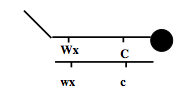
\includegraphics[width=.4\linewidth]{./img/01_cromosomiMais.png}
  \caption{Prima del crossing-over}
  \label{fig:sub1}
\end{subfigure}%
\begin{subfigure}{.5\textwidth}
  \centering
  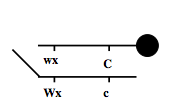
\includegraphics[width=.4\linewidth]{./img/02_crossingoverMais.png}
  \caption{Dopo il crossing-over}
  \label{fig:sub2}
\end{subfigure}
\caption{Cromosomi omologhi di mais presentanti marcatori genetici e citogenetici}
\label{fig:test}
\end{figure}

In seguito al crossing-over vi sarà la ricombinazione e il conseguente ottenimento di una progenie ricombinante. I ricombinanti, dal punto di vista fenotipico, avranno delle cariossidi:

\begin{itemize}
\item wx – C;
\item Wx –c.
\end{itemize}

Analizzando il cariotipo delle cariossidi ricombinanti sarà possibile osservare che i cromosomi hanno effettuato la ricombinazione poiché tra i due è avvenuto uno scambio fisico dei segmenti cromosomici; essi risulteranno infatti morfologicamente distinguibili.\\
L’esperimento appena spiegato rappresenta quindi una prova diretta che i geni si trovino sui cromosomi.

Un esperimento analogo venne effettuato nel 1931 da Stern, utilizzando il cromosoma X di Drosophila. I marcatori presi in considerazione furono:
\begin{itemize}
\item \textbf{carnetion (car)}, indicante il colore dell’occhio;
\item \textbf{bar (b)}, indicante la forma dell’occhio. 
\end{itemize}

In Drosophila l’allele dominante è indicato con il simbolo ``+'', mentre il recessivo con la sigla del gene coinvolto.
I cromosomi parentali presenteranno cromosomi X diversi: uno formato da due frammenti e l’altro con un prolungamento della regione centromerica. 
Anche in questo caso, come per il mais, l’individuo sarà un eterozigote strutturale ed eterozigote per carnetion e bar.

\begin{figure}[h]
\centering
\begin{subfigure}{.5\textwidth}
  \centering
  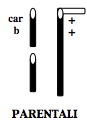
\includegraphics[width=.3\linewidth]{./img/03_cromosomiDrosophila.png}
  \caption{Prima del crossing-over}
  \label{fig:sub1}
\end{subfigure}%
\begin{subfigure}{.5\textwidth}
  \centering
  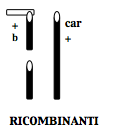
\includegraphics[width=.4\linewidth]{./img/04_crossingoverDrosophila.png}
  \caption{Dopo il crossing-over}
  \label{fig:sub2}
\end{subfigure}
\caption{Cromosomi omologhi di Drosophila presentanti marcatori genetici e citogenetici}
\label{fig:test}
\end{figure}

In seguito alla ricombinazione si otterrà un tipo ricombinante b/+ o car/+, ma anche cromosomi ricombinanti.

Questo esperimento dimostra, ancora una volta, che i cromosomi rappresentano la sede dei geni.


\subsection{Immagini}

\begin{figure}[h]
\centering
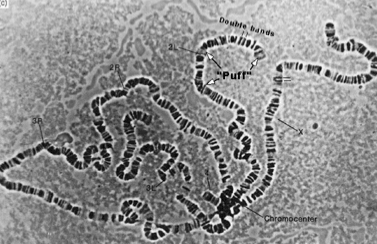
\includegraphics[scale=0.40]{img/04_cromo.png}
\caption{Immagine in contrasto di fase di cromosomi politenici non colorati}
\label{}
\end{figure}

\begin{figure}[h!]
\centering
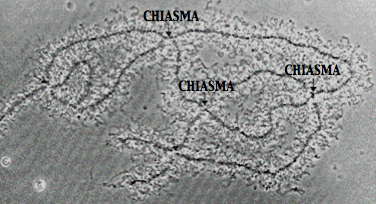
\includegraphics[scale=0.40]{img/05_cromospazzola.png}
\caption{Cromosomi a spazzola o lamp-brush, si tratta di cromosomi giganti che hanno avuto una particolare importanza per lo studio della sintesi dell’RNA. Sono presenti in tutti gli organismi, ma sono ben distinguibili in Xenopus laevis}
\label{}
\end{figure}

\begin{figure}[h!]
\centering
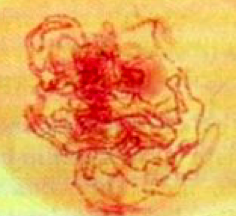
\includegraphics[scale=0.50]{img/06_cromopachitenespazzola.png}
\caption{Cromosomi in pachitene, una delle fasi della prima profase meiotica. Anche in questo caso si tratta di cromosomi a spazzola, ma non altrettanto ben studiabili come quelli giganti di Xenopus}
\label{}
\end{figure}

\begin{figure}[h!]
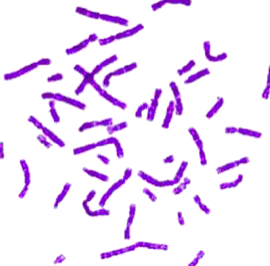
\includegraphics[scale=0.50]{img/07_cromoumani.png}
\centering
\caption{Colorazione standard di cromosomi umani in metafase. I cromosomi sono colorati in modo uniforme con un colorante affine al DNA}
\label{}
\end{figure}

\begin{figure}[h!]
\centering
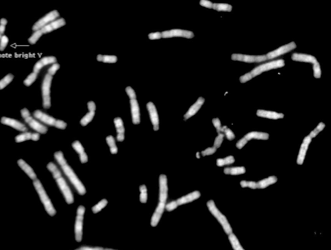
\includegraphics[scale=0.50]{img/08_cromobandeggi.png}
\caption{Particolarmente importante fu l’introduzione delle tecniche di bandeggio. Questa immagine mostra uno dei primi bandeggi storicamente sviluppati all’inizio degli anni `70 nel quale è possibile osservare delle regioni trasversali più o meno intensamente fluorescenti}
\label{}
\end{figure}

\begin{figure}[h!]
\centering
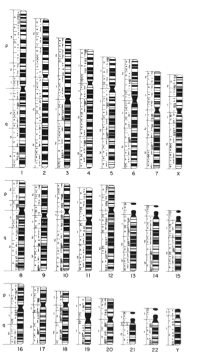
\includegraphics[scale=1.0]{img/09_cariotipo.png}
\caption{Successivamente vennero sviluppati altri bandeggi, questi furono fondamentali per l’identificazione dei cromosomi e per lo studio delle patologie cromosomiche. 
Per il riconoscimento dei cromosomi si utilizzano degli ideogrammi, questi rappresentano uno schema e vengono usati come riferimento per la descrizione di un cariotipo. Nell’ideogramma ogni banda rappresenta una rata(?) in modo tale che quando viene descritto un ri-arrangiamento cromosomico sarà possibile definire su che cromosoma ci si trova (braccio corto o lungo) e quali bande coinvolgano i punti di rottura.
Viene inoltre utilizzata una classificazione internazionale in modo che la descrizione del cariotipo sia universalmente comprensibile.
L’immagine a fianco mostra l’ideogramma di una metafase in cui la risoluzione è di sole 450 bande e una in cui invece la risoluzione è di 1700 bande. Non si tratta di una risoluzione elevata se si pensa che con i massimi livelli si arriva a distinguere fino a 3000 bande su un cariotipo umano. Sarà quindi possibile descrivere anche dei dettagli di riarrangiamenti molto piccoli, ciò risulterà essere fondamentale in molte patologie, ma soprattutto nel cancro}
\label{}
\end{figure}

\begin{figure}[h!]
\centering
\begin{subfigure}{.5\textwidth}
  \centering
  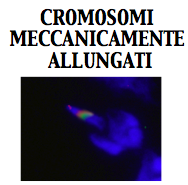
\includegraphics[width=.7\linewidth]{img/10_cromoallungati.png}
  \caption{}
  \label{fig:sub1}
\end{subfigure}%
\begin{subfigure}{.5\textwidth}
  \centering
  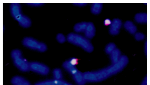
\includegraphics[width=1.1\linewidth]{img/11_cromoallungati.png}
  \caption{}
  \label{fig:sub2}
\end{subfigure}
\caption{Nell’immagine è possibile osservare l’utilizzo di una tecnica molecolare che permette di identificare determinate regioni cromosomiche con delle sonde molecolari. E’ possibile osservare una sonda marcata in verde e una in giallo. 
È possibile aumentare la risoluzione, potendo così cogliere più dettagli, utilizzando una tecnica che permette di stirare come degli elastici i cromosomi, nota come tecnica dei cromosomi meccanicamente allungati. }
\label{fig:test}
\end{figure}

\begin{figure}[h!]
\centering
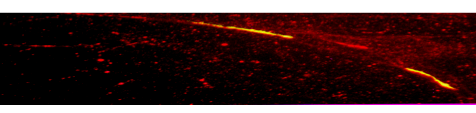
\includegraphics[scale=0.80]{img/12_cromatinapettinata.png}
\caption{Vi sono poi delle tecniche che permettono di pettinare la cromatina sui vetrini, di stabilire come siano disposte le diverse sequenze, quali siano i rapporti relativi (cosa si trova a destra piuttosto che a sinistra) e anche la distanza tra le diverse sequenze}
\label{}
\end{figure}

\begin{figure}[h!]
\centering
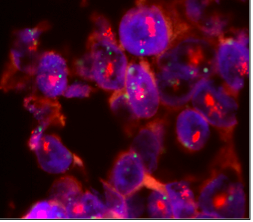
\includegraphics[scale=0.70]{img/13_celltumorali.png}
\caption{Nell’immagine a fianco è possibile osservare un caso di identificazione, con approcci molecolari, di regioni amplificate nel cancro alla mammella. Ciò risulta essere fondamentale perché permette di capire quale sia il grado di progressione della patologia.
Il gene marcato in rosso risulta essere molto amplificato nelle cellule tumorali, rappresenterà quindi una fase avanzata della malattia. 
Questo tipo di indagine è fondamentale perché permette di capire il livello di gravità e progressione del tumore, ma anche di fare la stessa analisi al termine di un trattamento terapeutico per osservare se vi sia stata una regressione del tumore. }
\label{}
\end{figure}


\begin{figure}[h!]
\centering
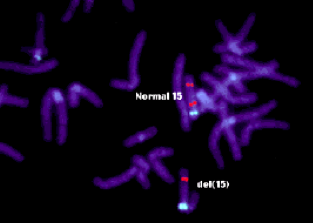
\includegraphics[scale=0.60]{img/14_microdelezioni.png}
\caption{La citogenetica molecolare può essere utilizzata anche per identificare delle micro-delezioni che non sarebbero visibili neppure con i  bandeggi ad alta risoluzione. L’immagine mostrante questa tecnica fa riferimento alla sindrome di prader-willi, molto studiata a causa del fenomeno dell’imprinting genomico}
\label{}
\end{figure}

\begin{figure}[h!]
\centering
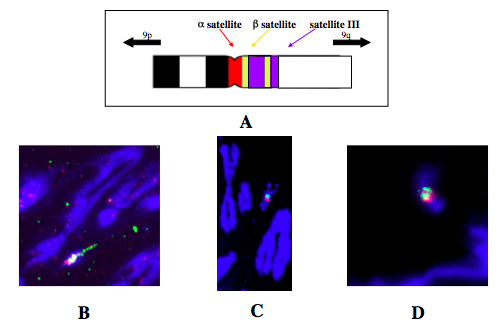
\includegraphics[scale=0.50]{img/15_cromoartificiale.png}
\caption{L’immagine a fianco mostra il lavoro che è stato fatto nel laboratorio della docente, in cui è stata fatta una mappa ad alta risoluzione della regione centromerica di un cromosoma umano, osservando quale fosse la sequenza e l’organizzazione dei diversi satelliti centromerici in una condizione normale e dopo aver costruito, attraverso delezioni successive, un cromosoma artificiale. 
Con i diversi gradi di risoluzione è possibile osservare i rapporti tra le diverse sequenze e la presenza/assenza di alcune delle stesse, marcate in fluorescenza con colori differenti}
\label{}
\end{figure}


\begin{figure}[h!]
\centering
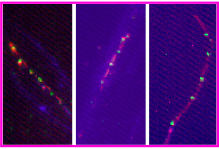
\includegraphics[scale=1.00]{img/16.png}
\caption{Nell’immagine sono stati analizzati i cromosomi allungati meccanicamente. In questo caso ciò che è interessante da osservare è non solo la struttura del centromero, ma anche la presenza di sequenze telomeriche. In questo caso era stato clonato, all’interno di un sito di clonaggio di un cromosoma artificiale, un gene marcatore (in verde nella figura) che risulta essere presente in 5 copie integrate}
\label{}
\end{figure}

\begin{figure}[h!]
\centering
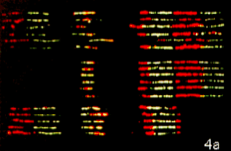
\includegraphics[scale=1.00]{img/17.png}
\caption{L’immagine a fianco mostra l’analisi di mutazioni del gene codificante per la distrofina su fibra di cromatina estesa.
Si tratta di un’immagine di un lavoro derivante dalla letteratura che prende in considerazione la distrofia di Duchenne. Il gene della distrofina è il gene più grande fino ad oggi clonato del genoma umano che quando mutato determina, appunto, la sindrome di Duchenne, una malattia invalidante abbastanza frequente. Risulterà quindi importante caratterizzare le diverse mutazioni sia per la diagnosi che per tentare degli approcci terapeutici mediante terapia genica.
In questo caso è stata costruita la mappa delle delezioni del gene della distrofina in diversi pazienti attraverso tecniche di citogenetica molecolare ad alta risoluzione grazie alle quali è possibile identificare i segmenti mancanti nelle differenti situazioni; ciò risulterà essere importante perché permetterà poi di vedere quali siano le delezioni più frequenti e, quindi, effettuare una diagnostica mirata}
\label{}
\end{figure}

\begin{figure}[h!]
\centering
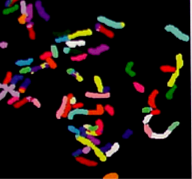
\includegraphics[scale=0.80]{img/18.png}
\caption{L’immagine a fianco mostra l’utilizzo di tecniche molecolari a più colori che permettono di colorare i cromosomi in modi differenti e di effettuare delle analisi in cui i ri-arrangiamenti cromosomici, anche molto complessi, potranno essere identificati grazie proprio allo scambio di colori tra i cromosomi. 
Se ogni cromosoma possiede un colore proprio, sarà possibile trovare un cromosoma arlecchino formato da diversi tasselli di provenienza nota. 
Quando si ha a che fare con ri-arrangiamenti che possono avere anche 10-11 punti di rottura, è chiaro che un bandeggio non permette di capire quali siano i punti di rottura dei cromosomi coinvolti; queste nuove tecniche, note come sky fish o spectral karyotyping, permetteranno invece di vedere anche ri-arrangiamenti molto complessi e di indirizzare l’analisi e la ricerca degli esatti punti di rottura}
\label{}
\end{figure}

\begin{figure}[h!]
\centering
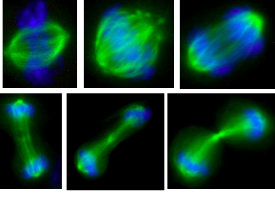
\includegraphics[scale=0.70]{img/19.png}
\caption{A fianco sono mostrate delle immagini di immunofluorescenza del fuso mitotico e dei cromosomi che permettono di osservare se vi siano delle anomalie di segregazione dei cromosomi rilevabili attraverso modificazioni della struttura del fuso mitotico. 
Generalmente si tratta di anomalie riguardanti il centromero}
\label{}
\end{figure}

\begin{figure}[h!]
\centering
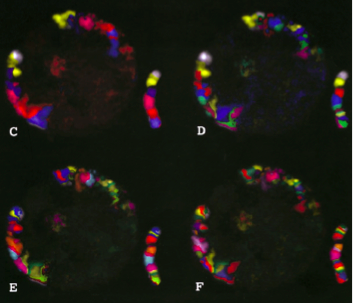
\includegraphics[scale=0.60]{img/20.png}
\caption{Ad oggi vi sono delle tecniche, risultanti fondamentali, che permettono di studiare i cromosomi nel nucleo interfasico. Nell’immagine è infatti possibile osservare dei nuclei
interfasici dove ciascuna banda di una particolare coppia di cromosomi è colorata in modo differente, sarà così possibile osservare l’organizzazione nel nucleo interfasico dei diversi distretti cromosomici. Ciò risulta essere molto importante perché è stato scoperto che la distribuzione tridimensionale dei vari domini cromosomici nel nucleo interfasico è direttamente correlata alla funzione degli stessi e che modificazioni della distribuzione si hanno nel corso del ciclo cellulare e possono anche essere indice di particolari perturbazioni dello stesso o di determinati pathway metabolici}
\label{}
\end{figure}

\begin{figure}[ht!]
\centering
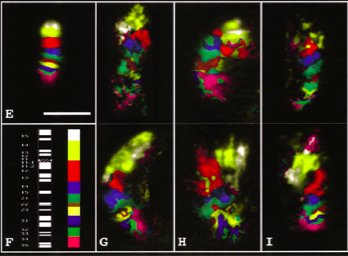
\includegraphics[scale=0.70]{img/21.png}
\caption{Queste tecniche permettono di fare un bandeggio cromosomico a più colori e vedere, nel nucleo interfasico, come sono organizzati i diversi distretti cromosomici. 
Questi approcci prevedono inoltre delle analisi tridimensionali del nucleo interfasico. È possibile arrivare a misurazioni e a simulazioni tridimensionali della disposizione di tutti i domini, queste risulteranno essere particolarmente importanti per fare delle deduzioni sull’importanza della posizione di particolari regioni cromosomiche nel nucleo interfasico e del loro significato funzionale}
\label{}
\end{figure}

\clearpage
La citogenetica del futuro è, fondamentalmente, la citogenomica; quest’ultima non vuole sostituire la citogenetica morfologica al microscopio, si tratta infatti di una disciplina che prevede l’utilizzo dei micro-array. Si parla quindi di citogenomica poiché rappresenterà un tipo di citogenetica fatta mediante approcci di genomica. 

\chapter{L'organizzazione del DNA}

A differenze dei procarioti, negli organismi eucarioti il grosso della regolazione dell'espressione genica avviene grazie a modificazioni del grado di condensazione del DNA, per questa ragione è molto importante conoscerne l'organizzazione.

In questo corso verranno approfonditi quei meccanismi che, modificando il grado di condensazione della cromatina (non è corretto parlare solo di DNA in quanto questo è complessato con le proteine istoniche), modulano la funzione delle cellule sia durante il ciclo cellulare che durante lo sviluppo e il differenziamento.
Il primissimo livello di regolazione dell’espressione genica negli eucarioti è dunque di carattere epigenetico. È evidente che siano importanti le sequenze regolatrici (promotori, enhancers, silencers, ecc), tuttavia l’attività di queste sequenze è modulata dalla loro accessibilità e quindi dal grado di condensazione della cromatina.

Prendiamo come punto di riferimento il genoma umano: nell’uomo la quantità totale in peso/massa di DNA è enorme, \emph{300 milioni bp} in aploidia. Se facciamo il conto, moltiplicando i 300 milioni per l’ingombro di ogni singola base, arriviamo ad una quantità di DNA pari a \textbf{1,80 metri} di lunghezza. Abbiamo dunque un'enorme sproporzione tra la dimensione del DNA e la dimensione del comparto in cui esso deve essere contenuto, e cioè il nucleo, il cui ordine di gradezza è quello dei micrometri. 

Si pone dunque il problema di come riuscire a condensarlo affinchè possa stare al suo interno: il DNA è una molecola molto sottile che potrebbe essere contenuta nel nucleo semplicemente comprimendola al suo interno ma, dal momento che circa ogni 24h il DNA di una cellula deve essere ripartito correttamente in due cellule figlie, è evidente che questo non può essere una matassa caotica ma deve essere rapidamente districabile. 
Il DNA raggiunge il suo massimo grado di condensazione durante la divisione cellulare (condensazione massina in metafase) e i cromosomi diventano dei ``gomitolini'' ben distinti con un livello di condensazione tale da renderli morfologicamente ben delineati e facilmente identificabili e classificabili al microscopio.

Il DNA è diviso in cromosomi, e negli essere umani la lunghezza totale di 1,80 metri è divisa in 23 coppie di cromosomi. Nell'organizzazione del DNA è poi molto importante che regioni che sono in qualche modo funzionalmente correlate ma linearmente molto distanti tra di loro, debbano potersi trovare vicine in certi momenti del ciclo cellulare, dello sviluppo e/o del differenziamento, in modo da poter essere espresse o replicate (replicazione e espressione sono fenomeni concertati) in maniera coordinata. È dunque fondamentale l'esistenza di meccanismi che permettano a tratti di DNA che, se consideriamo la molecola lineare, sarebbero molto distanti tra di loro di trovarsi in condizione di poter rispondere agli stessi segnali regolativi: si tratta fondamentalmente di meccanismi epigenetici di regolazione dell’espressione genica.

Qual è la soluzione ai problemi che abbiamo esposto? Com'è possibile che tutto il DNA entri nel nucleo?
Per risolvere questo problema il DNA viene condensato in modo ordinato, secondo una sequenza gerarchica di superavvolgimenti.
In generale il modello che viene seguito è il \textbf{modello a spirale}, un modello molto frequente in biologia e in tutto il mondo naturale in quanto, dal punto di vista fisico, è un modello energeticamente economico, ovvero è il modello che permette di ottenere forme ordinate con il minor dispendio di energia.


Vediamo alcuni rapporti tra dimensione del genoma e dimensione del comparto in cui questo è contenuto:
\begin{itemize}
\item Il \textbf{virus del mosaico del tabacco} è un virus filamentoso la cui dimensione è di 0.008 x 0.3  micron. Ha un genoma la cui lunghezza è di 6.4 Kb che corrispondono a 2 m. In questo caso non c’è una sproporzione così esagerata tra dimensioni del comparto/cellula/virus e dimensioni del genoma.
\item Il \textbf{Fago T4}, una cellula icosaedrica, ha una dimensione di 0.065 x 0.10 microm. Qui la sproporzione è già più evidente perché il genoma è di 170 Kb, per una lunghezza di 55 m.
\item \textbf{E. coli} è un batterio cilindrico tra i più conosciuti in quanto ampiamente utilizzato come organismo modello, della dimensione di 1.7 x 0.65 m. Il suo genoma è costituito da 4.2 x 103 Kb e ha una lunghezza di 1.3 mm (non più m).
\item Il \textbf{genoma umano aploide} è di \textbf{3x10\(^9\) Kb}, un genoma diploide è di 6 x 10\(^9\) Kb pari ad 1.80 metri. Il DNA umano è poi suddiviso in 46 cromosomi, ognuno dei quali è costituito da una molecola di DNA di circa 8 cm (la dimensione dei cromosomi è variabile), mentre il nucleo somatico sferico ha una dimensione di 6 micron (i nuclei delle cellule uovo sono molto più grandi).
\end{itemize}

La sproporzione tra la dimensione del genoma e quella del comparto in cui deve essere contenuto è evidente in tutti gli organismi e in particolare negli eucarioti superiori.
Una cosa fondamentale è che la cromatina, nelle cellule eucariotiche, viene trascritta e replicata in interfase.

Dal punto di vista energetico invece la fase più dispendiosa per la cellula è quella della divisione vera e propria, quando tutto il macchinario cellulare è concentrato sulla ipercondensazione della cromatina, sulla costruzione del fuso mitotico, sulla costruzione del cinetocore e su tutti quei processi che permettono la corretta separazione dei cromosomi nelle cellule figlie. Quando la cellula si divide la cromatina è ipercondensata: non viene né trascritta né replicata, salvo rarissime eccezioni.
Tutta l’attività metabolica della cellula invece si svolge durante l’interfase, quando il DNA è sì condensato perché deve stare nel nucleo, ma il grado di condensazione della cromatina è tale da consentire la funzionalità e la regolazione dell’espressione genica. 


\section{La cromatina}
Quando ci si riferisce agli eucarioti non bisognerebbe mai parlare di DNA ma di cromatina, in quanto normalmente il DNA è complessato con le proteine istoniche e solo transitoriamente è ``nudo''.

Gli istoni sono le proteine più abbondanti nel nucleo di una cellula eucariotica (rapporto in massa tra DNA e istoni di 1 a 1).

La cromatina viene divisa in \emph{eucromatina} ed \emph{eterocromatina}. Questa divisione è basata su osservazioni di microscopia ottica e si riferisce alla colorabilità con coloranti basici di diverse regioni del nucleo interfasico, distinguiamo:
\begin{itemize}
\item \emph{regioni più intensamente colorabili} che sono quelle più condensate durante l’interfase e sono le \textbf{regioni eterocromatiche}; 
\item \emph{regioni meno colorabili}, che sono quelle meno condensate durante l'interfase e sono le \textbf{regioni eucromatiche}.
\end{itemize}

Queste sono in realtà delle grosse generalizzazioni perché si basano soltanto su analisi morfologiche al microscopio ottico. In realtà, le regioni eucromatiche, come anche quelle eterocromatiche, contengono al loro interno rispettivamente regioni eterocromatiche e regioni eucromatiche: si tratta quindi di sub-regioni.

A sua volta l’eterocromatina si divide in:
\begin{itemize}
\item \textbf{eterocromatina costitutiva}. Questa è un'eterocromatina di tipo costituzionale, sempre presente a prescindere dalle fasi dello sviluppo, del differenziamento e del ciclo cellulare in cui una cellula di una certa specie si trova. Rappresenta una \emph{caratteristica intrinseca di una certa regione del genoma}. Questo tipo di eterocromatina è sempre presente in una determinata regione del genoma in tutte le cellule di tutti gli organismi della stessa specie.\\
In realtà ad oggi questo concetto è stato ampiamente messo in discussione.
Esempio eclatante: quando parliamo di eterocromatina costitutiva tipicamente ci vengono in mente le regioni centromeriche di tutti i cromosomi, ma oggi sappiamo che la regione centromerica non è completamente eterocromatica anzi, ad essere eterocromatica è la regione \emph{pericentromerica} che forma una sorta di barriera e che contiene al suo interno il core funzionale centromerico trascrizionalmente competente.
\item \textbf{eterocromatina facoltativa}. Questa eterocromatina è presente soltanto in certe condizioni, può variare, e quindi non caratterizza la struttura di una certa regione cromosomica. 
Questo tipo di eterocromatina può riguardare certe regioni del genoma solo in alcune cellule di alcuni organismi della stessa specie oppure può riguardare soltanto uno degli omologhi.\\
L’esempio meglio studiato di eterocromatina facoltativa è il cromosoma X inattivo nelle cellule somatiche delle femmine di mammifero (\textbf{N.B.:} l'inattivazione dell'X non riguarda solo l’uomo ma tutti i mammiferi e, più in generale, tutti gli organismi con eteromorfismo dei cromosomi sessuali).
Questo è l’esempio meglio studiato di eterocromatina facoltativa, ma in natura ce ne sono molti altri (per esempio in alcuni insetti vengono inattivati tutti i cromosomi di origine paterna nelle cellule somatiche dei maschi, e questo è un meccanismo di determinazione del sesso).
\end{itemize}

\begin{figure}[h!]
\centering
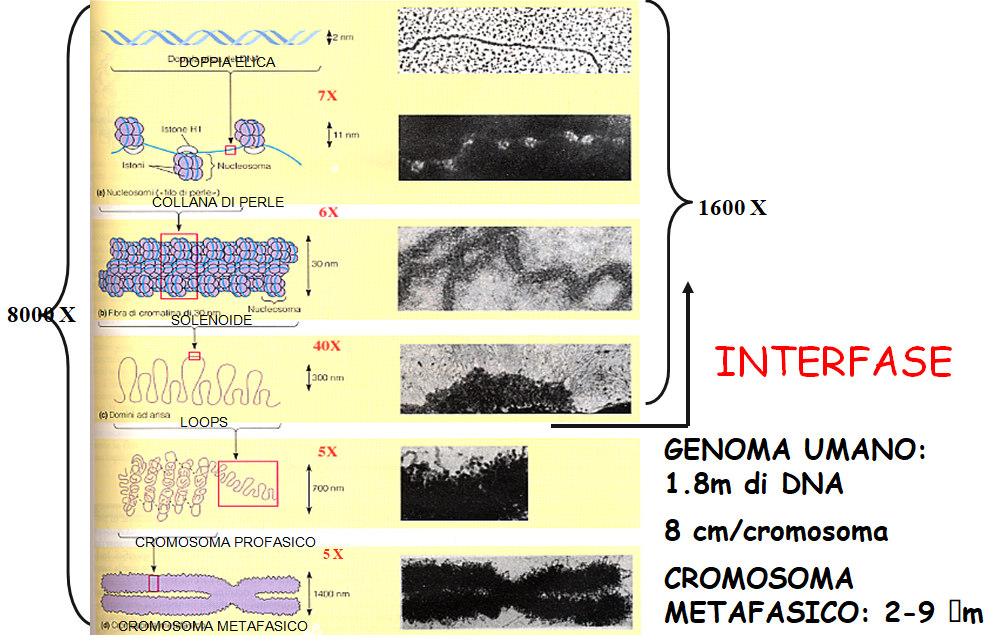
\includegraphics[scale=0.70]{img/22_cromatina.png}
\caption{Diversi livelli di condensazione del DNA. Possiamo vedere sia una rappresentazione schematica che l’immagine al microscopio elettronico. Inoltre nell’immagine si vede anche la dimensione, lo spessore, della fibra a cui ci riferiamo: il confronto di spessore delle fibre con ordine sempre superiore di superavvolgimento ci dà un’idea del grado di condensazione.}
\label{livelli_condensazione}
\end{figure}

Il ciclo di condensazione del DNA è rappresentato nell’immagine \ref{livelli_condensazione}, dove abbiamo una divisione molto netta tra ciò che riguarda l’interfase e ciò che riguarda invece le fasi successive all'interfase che portano alla divisione cellulare. La parte dell’interfase è quella che ci interessa di più perché è la fase in cui la cromatina funzionale è sì superavvolta ma in modo tale da poter comunque permettere la regolazione dell’espressione genica.\\
A partire dalla \emph{doppia elica} di DNA che ha un diametro di \textbf{20 \si{\angstrom}} (pari a 2 nm), passiamo alla struttura di ordine superiore che è la \emph{collana di perle} che si vede molto bene al microscopio elettronico e che ha un superavvolgimento di 7 volte per una dimensione di \textbf{11 nm}. Un’ulteriore condensazione di 6 volte porta dalla collana di perle alla \emph{struttura a solenoide} che ha un diametro di \textbf{30 nm}; si arriva poi alla \emph{struttura ad anse} che prevede un superavvolgimento di altre 40 volte per una dimensione di \textbf{300 nm} e una superavvolgimento totale di 1.600 volte per quanto riguarda la condensazione di DNA in interfase.\\
Le fasi successive seguono di nuovo un modello ad elica: abbiamo un superavvolgiemento di 5x5 volte che porta al cromosoma profasico e poi al cromosoma metafasico che raggiunge il massimo della condensazione.

Il modello seguito per il superavvolgimento è sempre quello a spirale:
\begin{itemize}
\item La doppia elica è un modello a spirale;
\item La collana di perle è un modello a spirale perché il DNA su ogni nucleosoma si superavvolge con due spire;
\item Il modello a solenoide è un modello a spirale perché in ogni giro del solenoide ci sono 6 perle della collana di perle;
\item Il \textbf{modello a loop} invece \underline{non è} un modello a spirale ma è un \emph{modello variabile}: a variare è sia la dimensione dei loop che il loro grado di affastellamento, di condensazione. È questa la parte più importante su cui ci soffermeremo perché ha un significato regolativo fondamentale.
\end{itemize}

Il processo di condensazione del DNA porta dunque da una fibra di 1,8 m a cromosomi singoli in cui mediamente il DNA è lungo 8 cm per cromosoma (in realtà, al microscopio, i cromosomi metafasici umani, ipercondensati, hanno una dimensione che varia da 2 a 9 micron circa).

Parliamo ora della struttura della cromatina: con questo termine ci si riferisce infatti alla fibra di DNA complessata con le proteine istoniche (basiche) con un rapporto in massa di 1:1.
Gli istoni sono in assoluto le proteine più abbondanti nel nucleo di una cellula eucariote.
La fibra elementare, e cioè la collana di perle, ha un diametro di circa 10-11 nm e deve il suo nome alla ripetizione assolutamente regolare di strutture globulari chiamate \textbf{nucleosomi}. Ogni nucleosoma/perla è poi legato all'altro da un segmento di DNA chiamato \textbf{DNA linker}.

I nucleosomi sono costituiti da un core proteico, che forma la struttura glomerulare, formato da un ottamero di istoni. Gli istoni sono 5: \textbf{H1}, \textbf{H2a}, \textbf{H2b}, \textbf{H3} e \textbf{H4}.
A formare il nucleosoma partecipano solo gli istoni\emph{ H2A, H2B, H3 e H4} con due subunità per tipo.\\
In questo momento l’istone H1 non partecipa ancora alla condensazione.

Su ogni nucleosoma si superavvolgono \textbf{2 spire di DNA} per un totale di circa \textbf{140-150 pb}.\\
Le perle poi sono unite tra loro da un ``filo'', che è il \textbf{DNA linker}, lungo circa \textbf{50 pb}.

\begin{wrapfigure}{r}{0.3\textwidth}
    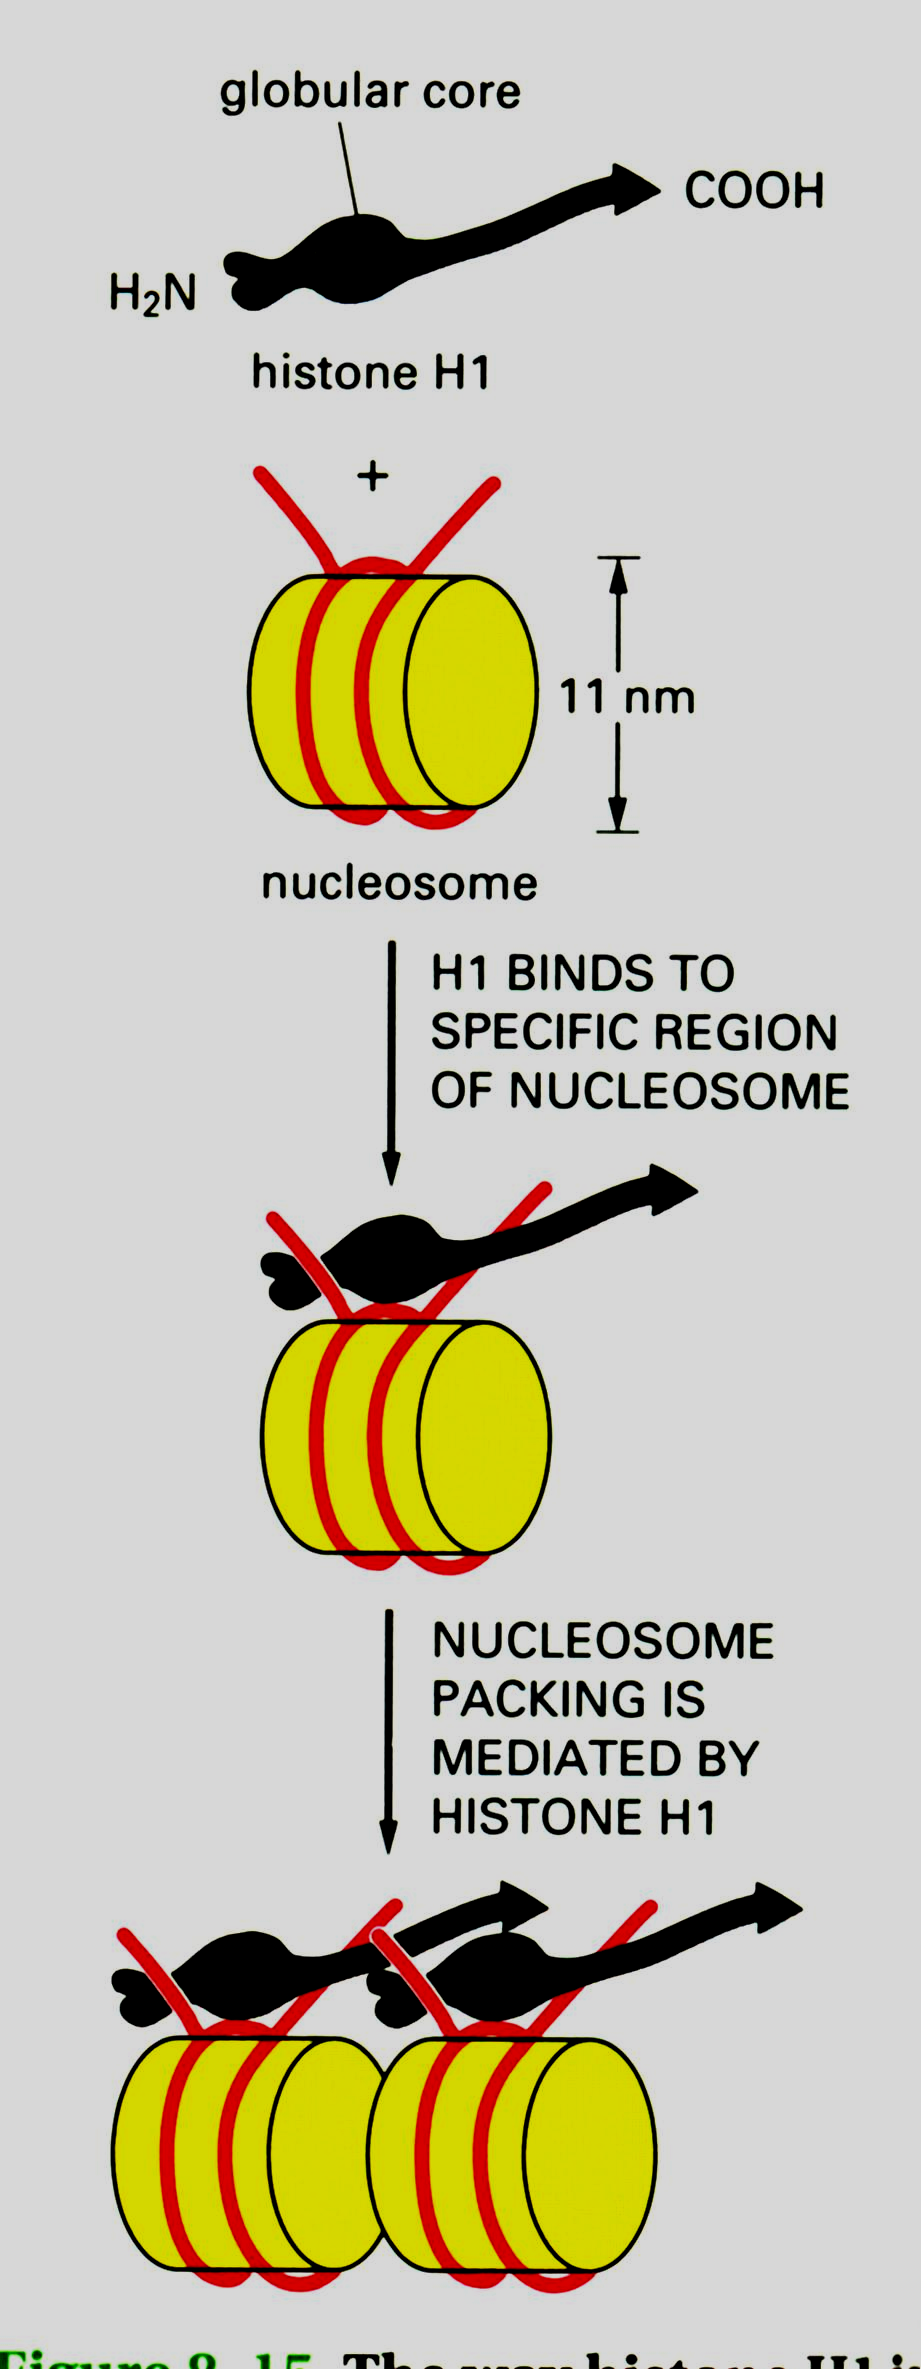
\includegraphics[width=0.27\textwidth]{img/23_histoneH1.png}
  \caption{Istone H1}
\end{wrapfigure}

L’\textbf{istone H1} invece si trova all’esterno rispetto all’ottamero e il suo compito è quello di collegare tra loro nucleosomi adiacenti determinando il superavvolgimento di ordine superiore, quello che porta alla formazione del \emph{solenoide}: in ciascun giro del solenoide si trovano \textbf{6 nucleosomi}, per portare alla struttura della fibra di 30 nm.

L’istone H1 nell’immagine di fianco è rappresentato come una specie di girino, con una testa (estremità C-terminale), una coda (estremità N-terminale) e una pancia. 
La pancia fornma la regione che interagisce con il DNA che si trova superavvolto sul nucleosoma, mentre la testa e la coda servono per i legami proteina-proteina che permettono la contrazione della fibra, in quanto l’istone H1 è legato all’esterno del nucleosoma attraverso un'interazione DNA-proteina.

Fino a questo livello di superavvolgimento c’è un motivo monotono ricorrente del modello a spirale che è più o meno uguale in tutti gli organismi e che segue questo ordine gerarchico. È un modello difficilmente modulabile fermo restando che, quando il DNA si deve replicare e deve essere trascritto, le proteine istoniche si devono staccare molto rapidamente per liberarlo.
Non è un caso che non abbiamo mai parlato di legami covalenti: queste sono tutte interazioni di tipo elettrostatico, fondamentalmente ponti H, proprio perché richiedono una bassa energia, sono facilmente reversibili e facilmente ricostruibili nel momento in cui si è compiuto il processo di replicazione e trascrizione.

\textbf{[DOMANDA:} il modello a zig-zag per quanto riguarda la fibra a 30nm non viene considerato? Il modello a zig-zag si ha quando il DNA linker ha una maggiore dimensione. Sono tutte variazioni sul tema: ci sono anche altri modelli più o meno validi e più o meno dimostrati, ma il modello più attendibile è quello a solenoide. Il modello a zig-zag si riferisce forse ad una sorta di ibrido tra il modello a solenoide e la struttura a loops.\textbf{]}

\subsection{La struttura a loops}

\begin{wrapfigure}{r}{0.3\textwidth}
    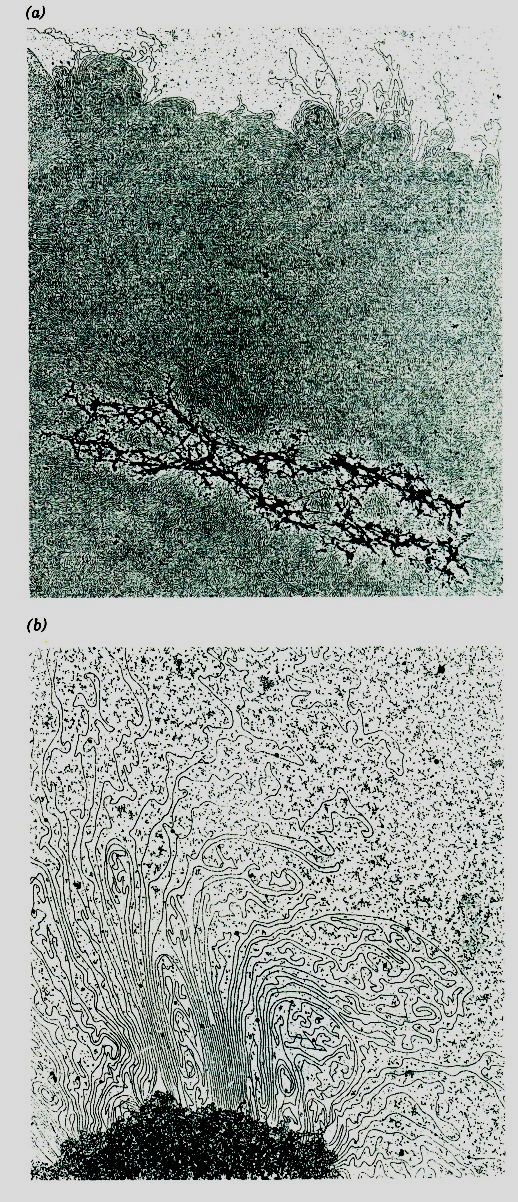
\includegraphics[width=0.30\textwidth]{img/25_backbone.png}
  \caption{Istone H1}
\end{wrapfigure}

È possibile trattare un cromosoma metafasico con una sostanza che permette di staccare gli istoni e che quindi permette la completa decondensazione (se tolgo gli istoni tutte le strutture di  ordine inferiore ovviamente si perdono). Osservando al microscopio elettronico il cromosoma metafasico trattato con questa sostanza vediamo che resta uno scheletro, chiamato \emph{``back bone''}, che rispecchia la morfologia del cromosoma metafasico. Tuttavia, a partire da questa sorta di colonna vertebrale che rimane, si vedono delle estensioni/estroflessioni che formano una sorta di alone intorno ad esso. Aumentando l’ingrandimento si può vedere come questo alone che si estroflette dal back bone sia costituito da fibre molto sottili che rappresentano delle anse continue: le anse si estroflettono a partire dallo scheletro per poi riattaccarvisi.\\
Queste analisi al microscopio elettronico sono la dimostrazione morfologica della struttura ad anse della cromatina, una struttura molto variabile e non sempre presente. Questa struttura, nonostante vari tra regioni diverse e a seconda della funzionalità, è effettivamente una struttura portante in metafase.
Quindi la cromatina interfasica ha una struttura ad anse.

Esistono delle evidenze della struttura ad anse: immagini in microscopia elettronica, esperimenti di sedimentazione, esperimenti di digestione con nucleasi. Tutti queste esperimenti hanno permesso di caratterizzare gli elementi di questa struttura.\\
Le anse sono delle \textbf{unità funzionali}: ci sono diverse prove sperimentali che dimostrano che le anse sono più o meno definibili come delle unità funzionali e cioè delle unità di trascrizione e di replicazione (eventi concertati). 
La struttura ad anse varia a seconda delle esigenze funzionali della regione cromosomica in un certo momento dello sviluppo e in un certo tipo cellulare. Ha un ruolo fondamentale nella regolazione dell’espressione genica e cioè nella trascrizione.

Regola generale, ma non sempre è così: tutto ciò che è attivamente trascritto è anche replicato all’inizio della fase S del ciclo cellulare, tutto ciò che è silenziato è invece replicato alla fine della fase S del ciclo cellulare.
Quello che è altamente condensato è poco trascritto ed ha replicazione tardiva. Quello che è poco condensato è attivamente trascritto ed ha replicazione precoce (durante la fase S iniziale). Questo avviene proprio perché trascrizione e replicazione sono processi metabolici interconnessi.

Lo scheletro proteico che è costituito dalla \textbf{topoisomerasi II}, la quale rappresenta la seconda proteina per abbondanza in massa nel nucleo delle cellule eucariotiche.

L’\emph{asse dell’ansa} è dunque il DNA complessato con gli istoni, mentre la \emph{base dell’ansa} è l’impalcatura che abbiamo visto bene nelle immagini di microscopia elettronica, chiamata \textbf{chromosome scaffold} (matrice del cromosoma) e costituita fondamentalmente dalla topoisomerasi II.

Che la base delle anse sia formata da delle topoisomerasi non è un caso, infatto queste sono proteine fondamentali durante la replicazione e la trascrizione perchè capaci di indurre tagli a singolo e a doppio filamento fondamentali per rilassare le tensioni torsionali che si vengono a creare quando il DNA si decondensa e quando la doppia elica si svolge. Se la doppia elica venisse semplicemente svolta ed aperta si sviluppere una tensione che potrebbe causare delle rotture casuali della molecola di DNA: affichè questo non avvenga ci sono le topoisomerasi che inducono dei tagli mirati a singola elica che vengono poi saldati e servono ad evitare che queste tensioni torsionali portino ad anomalie e ad errori nella replicazione e nella trascrizione.

Il fatto che la topoisomerasi II si trovi alla base delle anse ha un senso se è vero che le anse sono delle unità di trascrizione e di replicazione. La topoisomerasi ha dunque sia una funzione strutturale che enzimatica.
   
 Inoltre l'organizzazione a loops ha un significato molto importante perché ovviamente, se noi creiamo un’ansa anche molto grande, facciamo in modo che regioni fisicamente molto lontane sulla molecola lineare di DNA vengano a trovarsi invece molto vicine.\\
L’organizzazione a loops è dunque in grado anche di tenere fisicamente vicine regioni che devono essere trascritte o replicate nello stesso momento funzionale: queste regioni potranno trovarsi fisicamente vicine per rispondere agli stessi segnali regolatori.

A questo punto, siccome il loop ha un significato regolativo, è facile capire come la dimensione e il grado di condensazione dei loop varino in diversi stadi dello sviluppo e in diversi tessuti.

\begin{wrapfigure}{r}{0.62\textwidth}
    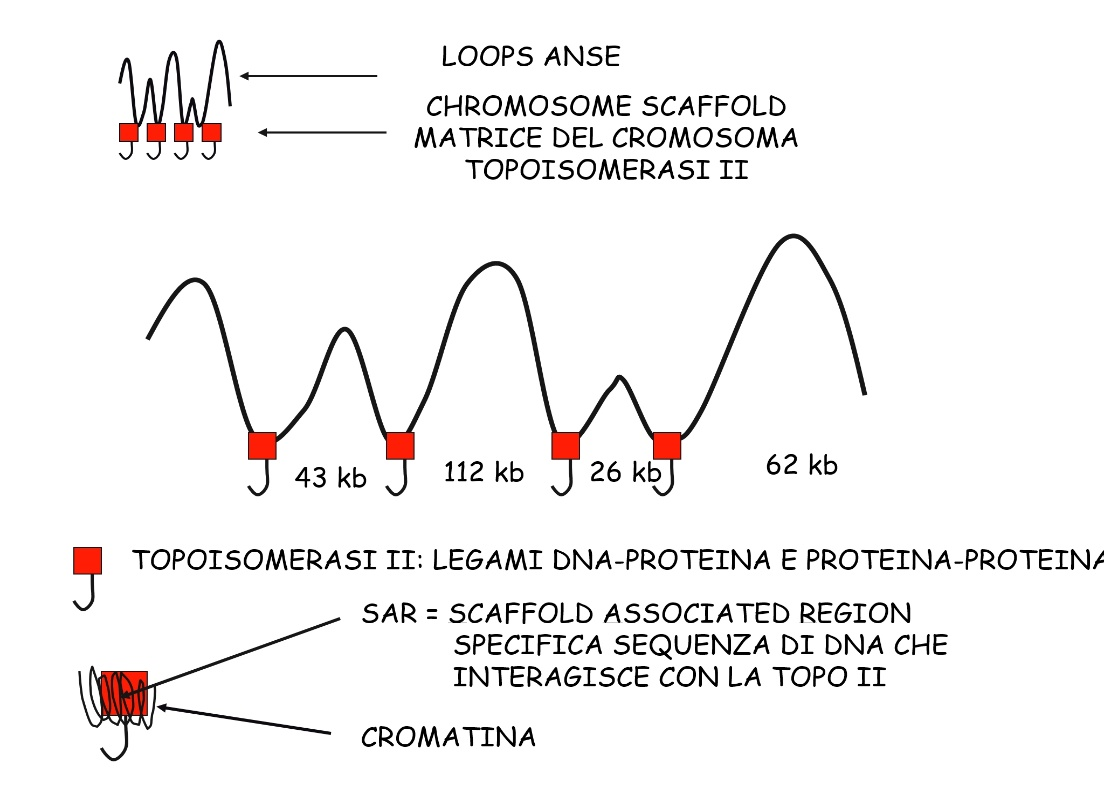
\includegraphics[width=0.60\textwidth]{img/26_anse.jpg}
  \caption{La topoisomerasi II e l'organizzazione ad anse}
\end{wrapfigure}

Il disegno a lato ci fa capire come la struttura a loops possa essere facilmente regolata e cioè come, grazie al legame della base delle anse con la topoisomerasi, siamo in grado di modulare la dimensione e il grado di affastellamento delle anse.\\
Nel disegno la topoisomerasi è rappresentata come una sorta di vagoncino con un occhiello: la parte rossa del vagoncino è quella su cui si trova la regione della topoisomerasi affine al DNA, e cioè la regione di interazione DNA-proteina: la parte rossa è legata alla base delle anse.\\
Il chromosome scaffold è dato dall’allineamento delle diverse molecole di topoisomerasi.

La topoisomerasi quindi è in grado di formare legami DNA-proteina che si trovano alla base dell’ansa, ma anche legami proteina-proteina che saranno i legami tra gli occhielli di molecole di topoisomerasi adiacenti. È evidente come questo permetta facilmente di modificare sia la dimensione che il grado di affastellamento dei loop.

Come faccio a modificare la dimensione dei loop?
Se ho due loop adiacenti, uno di 112 Kb e l’altro di 26 Kb, e tolgo la molecola di topoisomerasi compresa tra i due loop, succede che da due loop di quelle dimensioni ne ottengo uno più grande la cui dimensione sarà esattamente di 112 + 26 Kb.\\
Modulando semplicemente l’interazione DNA-proteina posso modulare la dimensione dei loop, mentre Per quanto riguarda il grado di condensazione è evidente che gli occhielli potranno interagire tra loro in modo lasso o stretto. La forza dell’interazione tra molecole di topoisomerasi adiacenti modulerà il grado di affastellamento dei loop e quindi il loro grado di condensazione.

Abbiamo detto che regione dove il DNA interagisce con la topoisomerasi si trova alla base dei loop, il DNA però può essere o meno legato alla topoisomerasi. Le regioni di DNA capaci di legarsi alle topoisomerasi si chiamano \textbf{SAR (Scaffold Associated Region)}.

Ciò che modula l'organizzazione ad anse è dunque l’interazione più o meno forte tra topoisomerasi (affastellamento), ma anche il legame o meno con la topoisomerasi (dimensione dei loop).

Ma se le regioni SAR sono sempre presenti, perché a volte legano la topoisomerasi  mentre altre volte no? È evidente che le stesse regioni SAR devono essere capaci o meno di legare la topoisomerasi, e questa capacità è determinata dalle modificazioni epigenetiche.\\
Epigenetica vuol dire che la stessa sequenza (o sequenze molto simili) può all’occorrenza trovarsi in una condizione tale da poter interagire con un fattore (in questo caso con una proteina) o meno.

La stessa molecola di topoisomerasi trova delle SAR disponibili o delle SAR incapaci grazie alla presenza di segnali chimici che rendeno le molecole di topoisomerasi in quella regione più affini rispetto a tutte le altre molecole di topoisomerasi. \emph{(la modificazione epigenetica è a livello delle SAR o della topoisomerasi??)}\\
Tutti questi sono segnali epigenetici perché la sequenza del DNA è sempre la stessa. Ad intervenire sono delle piccole molecole in grado di modificare localmente la struttura del DNA (in questo caso della SAR) rendendola aperta o chiusa, oppure di modificare la proteina rendendola più o meno affine alle altre proteine della sua stessa categoria.
Oggi sappiamo che queste piccole molecole sono RNA non tradotti. 

Questi cambiamenti epigentici sono essenziali se pensiamo che ogni loop è un'unità funzionale a sé stante. Nell'organizzazione del DNA possiamo fare una distinzione tra i geni housekeeping (geni che regola il metabolismo di base e che sono attivi in tutte le cellule) e geni tessuto-specifici.\\
I \textbf{geni housekeeping} regolano il metabolismo cellulare e sono trascritti in tutte le cellule ad un livello basale, mentre i geni tessuto-specifici vengono trascritti solo in certi tipi cellulari e sono trascritti a livelli molto più elevati.
A causa delle diverse esigenze di trascrizione l'organizzazione in loop di questi geni sarà diversa:
\begin{itemize}
\item i \textbf{geni housekeeping}, in generale, si trovano in loop piuttosto grandi e abbastanza condensati perché devono essere trascritti in maniera basale in tutte le cellule di tutti gli organismi. Nelle zone di \emph{eterocromatina costitutiva}, completamente inerti, troviamo loop molto grandi e molto molto condensati.
\item i \textbf{geni tessuto-specifici} invece si troveranno in loop piccoli e molto lassi (i.e. loop in cui si trova fondamentalmente un solo gene che viene continuamente trascritto). Quella stessa regione nella cellula di un altro tessuto sarà ipercondensata.
\end{itemize}

Se nei loop piccoli troviamo un solo gene o quasi e di conseguenza la trascrizione risulta molto rapida, i loop grandi conterranno unità trascrizionali che, venendo trascritte in sequenza, necessiteranno di tempi più lunghi.
Bisogna sempre ricordare che, durante la trascrizione e la replicazione, la doppia elica del DNA si deve aprire e i nucleosomi si devono staccare in maniera transiente per poi riattaccarsi subito dopo perché il DNA deve essere accessibile al complesso trascrizionale o al complesso replicativo. Affinchè questo avvenga, la cromatina deve essere in una conformazione adatta: si devono rapidamente staccare gli 8 istoni che formano il nucleosoma ma, appena completato il processo di trascrizione e di replicazione, gli istoni dell’ottamero si devono riassociare al DNA e tutto questo è modulato dalla struttura ad anse.
Le anse sono più o meno compatte e più o meno grandi nei diversi momenti funzionali e in diverse regioni cromosomiche: questo è variabile per le esigenze del differenziamento e dello sviluppo.

Il significato funzionale dei loop è dimostrato anche dal fatto che le SAR normalmente si trovano vicine ai promotori: facendo un trattamento con enzimi di restrizione, considerando anche elementi regolativi a lunga distanza come gli enhancers, è molto facile che sullo stesso frammento di restrizione si trovino sia una SAR che un elemento regolativo a lunga distanza (enhancer).

Cosa sono le modificazioni epigenetiche?\\
Sono cambiamenti della cromatina che regolano l’espressione genica a livello trascrizionale.
Tra i vari livelli di regolazione dell'espressione genica quello più economico è quello che interviene già a livello della trascrizione in quanto evita sprechi metabolici ed energetici.

Le modificazioni epigenetiche non alterano la sequenza del DNA ma la struttura tridimensionale della cromatina, hanno un ruolo chiave nei processi di regolazione dell’espressione genica negli eucarioti e rappresentano il sistema più usato per regolare l’espressione genica.
Le modificazioni epigenetiche non riguardano promotori, enhancers e silencers di per sé, ma piuttosto l’accessibilità di tali sequenze ai fattori con cui interagiscono. Le modificazioni epigenetiche fanno in modo che le sequenze regolatrici siano o meno capaci di interagire con i propri effettori.

Queste modificazioni consistono fondamentalmente in:
\begin{itemize}
\item metilazione del DNA;
\item metilazione ed acetilazione di specifici gruppi degli istoni che formano l’ottamero.
\end{itemize}

Una cosa fondamentale è che in ogni regione del genoma degli eucarioti superiori esiste un rapporto ben preciso tra grado di metilazione e grado di acetilazione e addirittura questo rapporto locale tra numero di acetili e numero di metili rappresenta una sorta di \textbf{codice istonico} che si sovrappone al codice genetico, proprio perché ha la capacità di modulare l’espressione genica locale. In qualche caso il codice istonico è stato decodificato: ci sono delle regioni del genoma in cui si è stabilito esattamente qual è il rapporto chiave tra metili e acetili e quindi il codice istonico per avere un certo livello di espressione genica. 

Le SAR sono state facilmente isolate e caratterizzate trattando il DNA con la stessa sostanza usata per ottenere il back bone proteico (litio 3’, 5 diiodiosalcilato, LIS), ovvero una molecola capace di rimuovere gli istoni. Rimuovendo gli istoni vi saranno delle regioni che risulteranno protette dal trattamento con enzimi di restrizione perché schermate dalla topoisomerasi. A questo putno posso rimuovere la topoisomerasi e caratterizzare i segmenti di DNA che erano stati protetti dalla digestione enzimatica: in questo modo sono state sequenziate le SAR.
Tutti questi esperimenti sono stati fatti fondamentalmente in Drosophila melanogaster.
Questo permette anche misurare la dimensione dei segmenti che si trovano tra due regioni protette dalla digestione enzimatica e quindi valutare la dimensione dei loops e dunque la distanza tra SAR adiacenti. In Drosophila la dimensione dei loops è molto variabile: da 4,5 a 115 Kb.


Tutte le SAR studiate contengono da 8 a 17 box ricorrenti: per \emph{``box''} si intende un blocco di sequenza: questi blocchi sono specifici e ricorrenti, molto simili tra loro in SAR diverse.\\
In tutte le SAR è presente un \emph{sito di legame per la topoisomerasi} costituito dalla sequenza \textbf{GNT(A/T)A(T/C)ATTNATNN(G/A)}. 
Vi sono poi altre due box ricorrenti (tra quelle trovate confrontando le diverse SAR della Drosophila melanogaster) dal significato regolativo: sono presenti o assenti a seconda che ci troviamo in una regione di geni housekeeping (che non devono essere regolati perché son trascritti in tutte le cellule di tutto l’organismo) o di geni tessuto-specifici (regolati). Abbiamo quindi una \textbf{T-box} che è una \textbf{sequenza ricca in T} ed una \textbf{A-box} che è \emph{ricca in A}. La T-box si trova a valle della A-box. La differenza tra geni housekeeping e geni  tessuto-specifici sta proprio in queste box regolative:
\begin{itemize}
\item i geni housekeeping non sono regolati perchè trascritti a livello basale in tutti i tessuti e in tutti gli stadi del differenziamento, hanno delle SAR costitutive sempre legate alla topoisomerasi che mancano della A-box.
\item i geni tessuto-specifici invece presentano SAR che devono essere regolate perchè trascritti ad alto livello soltanto in certi tessuti e presentano la A-box.
\end{itemize}



\chapter{La localizzazione dei geni sui cromosomi}
L’importanza di localizzare i geni sui cromosomi costruendo delle mappe genetiche non è solo di tipo topografico. 
Le prime mappe sono state costruite ordinando sui cromosomi dei geni noti. 
Uno degli esperimenti storici di mappaggio dei geni è stato fatto in Drosophila, ed il primo cromosoma ed essere stato mappato è stato l’X. Questi esperimenti sono stati fatti con un approccio di tipo genetico calcolando la \emph{distanza dei geni sulla base delle frequenze di ricombinazione}. Il metodo che venne utilizzato fu quello dell’incrocio a tre punti, il quale permette di stabilire in base alla frequenza di ricombinazione la distanza dei geni. La frequenza di ricombinazione di due geni è proporzionale alla distanza e dunque alla probabilità che questi vengano separati da un evento di ricombinazione: è un \emph{approccio di tipo statistico}.
Poichè il metodo statistico non ci da un’informazione sulla distanza lineare (i.e. numero di paia di basi) tra due geni, questa può essere trovata anche tramite un approccio di tipo fisico.

Mappare i cromosomi significa soprattutto identificare nuovi geni, e identificare la distanza tra due o più geni ci permette sia di capire come questi interagiscono tra loro ma anche di identificare segnali regolativi che ne influenzano l’espressione.

Al significato topografico si aggiungono degli elementi che permettono di fare delle deduzioni sul funzionamento di questi geni in base al loro rapporto di linkage: l’identificazione di blocchi di geni altamente conservati e nello stesso linkage lascia presupporre che questi ultimi abbiano attività estremamente correlate tra loro e che abbiano anche avuto un importante significato evolutivo.

Ad oggi grazie agli approcci post-genomici è possibile allineare su un genoma degli enormi segmenti di DNA, e ciò su cui ci si sta concentrando è cercare di stabilire i ruolo di singole sequenze, come queste interagiscano le une con le altre e come rispondano agli stessi segnali regolativi. Ad oggi è possibile arrivare fino alla determinazione della sequenza con Sanger oppure con gli approcci di NGS (rapido sequenziamento di genomi complessi).

A cosa serve costruire una mappa?
\begin{enumerate}
\item conoscere la topografia del genoma consente di \textbf{prevedere e controllare l’eredità dei caratteri}
\item si possono costruire dei modelli di regolazione dell’espressione genica basati sulla presenza di sequenze regolatrici, ma si possono anche \textbf{costruire dei modelli di regolazione epigenetica} proprio perché il fatto che dei geni si trovino in particolari domini genomici fa in modo che questi abbiano un tipo di regolazione simile e quindi rispondano in maniera simile agli stessi segnali regolatori
\item \textbf{studiare le interazioni tra i geni}
\item \textbf{studiare l’organizzazione del genoma}: nell’era post-genomica, dopo il sequenziamento grezzo del genoma (terminato nel 2001), si è aperto un nuovo mondo grazie alla scoperta di tantissime sequenze che non sono codificanti ma che hanno un ruolo chiave nella regolazione dell’espressione genica
\item \textbf{studiare l’evoluzione dei genomi}: fare un’analisi comparata della topografia di genomi più o meno correlati evolutivamente permette di capire quali siano i meccanismi molecolari che governano l’evoluzione dei genomi.
\end{enumerate}

Questi sono approcci fondamentali per completare le informazioni statistiche che vengono dal mappaggio dei genomi con le tecniche di NGS, che hanno l’enorme limite di essere approcci statistici che vanno verificati. A tal proposito di si parla si \textbf{dry laboratory approches} e \textbf{wet laboratory approches}. I primi, quelli in asciutto, sono quelli fatti con approcci bioinformatici analizzando banche dati, si basano su studi probabilistici che hanno bisogno di verifiche in bagnato, cioè sperimentali, in laboratorio.

Vediamo una panoramica dei metodi classici:
\begin{enumerate} 
\item \textbf{Mappaggio genetico (statistico)}
\begin{itemize}
\item \textbf{Analisi di linkage}. Queste analisi non sono soltanto utilizzate per l’identificazione dei geni malattia ma anche per capire se alcuni geni malattia sono più o meno correlati ad altri geni che ne influenzano la funzione (per questo è molto importante lo studio degli alberi genealogici). Lo studio di linkage non è altro che il trasferimento ad \emph{organismi nei quali \underline{non è possibile} fare incroci programmati} delle analisi di linkage classiche, che studiano i rapporti fra i geni e la loro distanza sulla base delle frequenze di ricombinazione. È evidente che un approccio del genere, nella Drosophila o nel mais, prevede la conoscenza di marcatori morfologici e la programmazione di incroci. In questi casi il numero di caratteri morfologici che possono essere studiati è enorme, è possibile programmare degli incroci e selezionare delle linee pure attraverso numerose fasi di incrocio (ovvero incrocio fra fratelli) per poi andare a studiare una progenie molta numerosa (numeri statisticamente rilevanti) con tempi di generazione che sono di alcune settimane. È evidente come questo metodo non possa essere trasferito ad organismi superiori (e.g. uomo e/o organismi di interesse zootecnico come i bovini) non solo perché è più complicato programmare gli incroci, ma anche per i tempi di generazione e la numerosità della progenie. Inoltre nell’uomo queste analisi non possono essere condotte non solo per i tempi di generazione (30 anni) ma anche perché il numero di caratteri morfologici è esiguo: negli studi di linkage è vero che nell’uomo si studierebbe la segregazione di geni malattia, ma lo studio di linkage prevede di studiare la co-segregazione del gene che ci interessa con un altro marcatore fenotipico facilmente identificabile e siccome nell’uomo non si può parlare di colore del pelo o cose del genere, questo è molto difficile.
 
Quindi, non potendo programmare gli incroci, le analisi di linkage nell’uomo consistono nello studiare degli incroci già avvenuti: \emph{analisi dei pedigree}. Questo tipo di analisi si fa su grandi o piccole famiglie purché si abbiano tante famiglie in cui segrega la stessa malattia e per poi analizzare la co-segregazione della malattia con dei marcatori di riferimento. Come marcatori si possono utilizzare diversi marcatori proteici, ad esempio oggi si usano marcatori del DNA che consistono fondamentalmente nei polimorfismi del DNA come ad esempio i polimorfismi RFLP, e cioè polimorfismi che riguardano la lunghezza di frammenti di restrizione: se si digerisce il DNA con un enzima di restrizione si ottiene una sonda che identifica quel segmento. Esistono dei polimorfismi che non hanno effetto fenotipico ma modificano la dimensione di questi frammenti, caratteristica di un individuo. Se un certo polimorfismo co-segrega sempre con il gene malattia avrò stabilito qual è l’aplotipo, ovvero il cromosoma che ha il gene malattia e questo mi permette di seguire la segregazione del cromosoma nella famiglia e fare delle deduzioni sulla probabilità che un individuo sia portatore del gene malattia (per fare poi della consulenza genetica). In realtà oggi non si usano quasi più gli RLFP ma si usano mutazioni anche di singoli nucleotidi, oppure polimorfismi che riguardano minisatelliti e microsatelliti. All’inizio quindi si usavano i polimorfismi proteici, oggi si usano i polimorfismi del DNA, microsatelliti, minisatelliti e SNPs. La citogenetica non si limita a determinare la distanza tra i geni e la probabilità che vengano trasmessi, ma è un approccio fisico.
\end{itemize}

\item \textbf{Mappaggio citogenetico molecolare}. Con questo approccio si riesce esattamente a stabilire dove si trova il gene sul cromosoma e a che distanza si trova da un particolare gene marcatore che ci interessa. Gli approcci di cui parleremo sono quelli di: 
\begin{itemize}
\item \textbf{mappaggio citologico} (sui cromosomi)
\item \textbf{studio della dose genica}, che ormai non si usa più
\item \textbf{ibridazione di cellule somatiche} - non solo è un approccio per la localizzazione genica molto potente ma è anche utile per spiegare come ibridi somatici siano quelli che permettono di produrre Ab monoclonali che sono il presente e il futuro della ricerca soprattutto nel campo della diagnostica precoce della terapia del cancro.
\item \textbf{ibridazione in situ}. Questa tecnica che negli ultimi 15-20 è arrivata a una potenzialità descrittiva che permette di sovrapporre questo approccio a quello del mappaggio fisico molecolare che consiste fondamentalmente nella costruzione di mappe di restrizione fino ad arrivare all’allineamento di Bach per il sequenziamento grezzo (detto draft genome sequencies). Le prime sequenze complete dei genomi vengono fatte attraverso l’allineamento di grossi contigui fino ad arrivare al sequenziamento vero e proprio. 
\end{itemize}
  
\item \textbf{mappaggio fisico} (molecolare, sulla sequenza):
\begin{itemize}
\item \textbf{mappe di restrizione} classiche
\item \textbf{mappe di restrizione “long range"}
\item \textbf{mappe di cloni di DNA contigui}
\item \textbf{sequenziamento del DNA}
\end{itemize}
\end{enumerate}

Le tecniche di ibridazione in situ, di ibridazione di cellule somatiche e di mappaggio fisico sono altamente complementari. Le prime due arrivano a una capacità di risoluzione che si avvicina alla singola base e dà informazioni anche di tipo architettonico (cosa c’è sopra, sotto, destra ecc..)

\section{Le analisi di linkage}
Questa tecnica consiste nello studiare nelle famiglie la co-segregazione di un gene malattia e di un marcatore. È una tecnica utile per identificare l’aplotipo, cioè la sequenza sul cromosoma legata alla trasmissione della malattia. Questo permetterà di studiare i polimorfismi del DNA e in base alla presenza o assenza di un polimorfismo si può capire se l’individuo è portatore del gene malattia o meno. Ciò è importante per scopi diagnostici, per la consulenza genetica e per lo studio nelle popolazioni dell’incidenza di una particolare mutazione. Nello studio di malattie ereditarie ma anche del cancro ci permetterà di sapere qual è la mutazione più frequente in quella particolare popolazione, e quindi cercare prima quella.

\section{Ibridazione di cellule somatiche} 
Nei mammiferi le cellule somatiche sono così altamente differenziate che difficilmente si adattano ad essere coltivate in vitro (non si replicano o lo fanno occasionalmente in risposta a un qualche stress o danno). Questi approcci complessivamente prendono il nome di \emph{``genetica di cellule somatiche''}.

Mentre con organismi quali lieviti e batteri è facile fare incroci e riconoscere rapporti di dominanza grazie agli svariati marcatori metabolici e alle capacità proliferative di queste cellule, nei mammiferi questo approccio è molto più difficile e presenta svariati limiti.\\
Fu il Prof. Pontecorvo a notare per primo che anche le cellule di mammifero possono andare incontro ad eventi di fusione (evento comune in procarioti e eucarioti unicellulari ma molto raro nei mammiferi). A seguito di questa osservazione vennero messi in coltura fibroblasti sottocutanei, i quali sono capaci di adattarsi e crescere in vitro come cellule isolate. Una volta che queste cellule sono adese ad un supporto (sono cellule che provengono da un tessuto solido, hanno dunque bisogno di una sorta di membrana basale a cui aderire per crescere, per questo vengono coltivate in piastra Petri) possono essere amplificate e congelate come colture cellulari.\\
A seguito di questa osservazione si pensò che fosse possibile considerare le colture di cellule somatiche come popolazioni di singole cellule, e che ogni cellula potesse essere considerata come un singolo organismo. Poichè ogni cellula possiede tutta l’informazione genetica dell’organismo da cui deriva si pensò di promuovere la capacità di fusione spontanea di queste ultime per poi analizzare l’ibrido, ottenendo così un risultato simile a quello di un incrocio.\\
È ovvio che questa tecnica presenta dei limiti rispetto ai batteri: non posso studiare molti caratteri morfologici ma ci sarà un limite a quelli che posso studiare perché si esprimono in cellula, sono caratteristiche morfologiche ma soprattutto metaboliche (espressione di marcatori proteici e forma della cellula per esempio). La genetica di cellule somatiche nasce dunque da quest’idea.

Viene definita \textbf{eterocarionte} una cellula che possiede: una sola membrana plasmatica, un solo citoplasma, due nuclei. Questa è una cellula eterogenea per quanto riguarda il carion, ovvero i nuclei.
A volte può succedere che anche i nuclei si fondano portando alla formazione di una nuova cellula nella quale il nucleo contiene entrambi i genomi completi delle cellule parentali. Questa sarà una cellula tetraploide detta \textbf{sincarionte}.

La fusione cellulare avviene spontaneamente in alcuni tessuti (e.g. nel fegato dove ha un significato importante perché si ottengono cellule poliploidi ad alta secrezione, nelle ghiandole e nel muscolo scheletrico, dove troviamo dei sincizi).

Poichè quello della fusione è un fenomeno raro nei mammiferi, sono state studiate delle tecniche che potessero aumentarne la frequenza. A questo scopo è stato studiato il \textbf{virus Sendai} (Sendai è una città del Giappone, il virus fu scoperto nel 1965), il quale è conosciuto anche come Virus Emoagglutinante del Giappone (HVJ). Questo virus ha la capacità di aumentare la fusione delle vescicole lipidiche e delle membrane cellulari collegando fra loro due membrane e creando un vero e proprio ponte citoplasmatico tra le due cellule (ovviamente queste si devono trovare fisicamente vicine). Il virus viene isolato da uova di pollo gallate (fecondate, le uova gallate poi marciscono) e poi inattivato tramite esposizione a luce UV. Ad oggi questo virus non è più utilizzato ma viene usato un polimero, con catena più o meno estesa, che è il PEG.

Il \textbf{PEG (Glicole Poli Etilenico)} è un polimero preparato per \emph{polimerizzazione dell'ossido di etilene}. Ne esistono diversi tipi classificati in base alla lunghezza media delle molecole (i.e. diverso PM. La scelta del peso molecolare dipenderà dalle cellule che abbiamo).\\
I diversi polimeri hanno differenti proprietà fisiche (e.g. la viscosità), inoltre sono un po' citotossici (ma non alle dosi usate per la fusione cellulare). Il PEG è affine alla membrana cellulare e idrosolubile, crea ponti citoplasmatici fra le cellule in contatto fisico e in questo modo promuove la fusione delle membrane cellulari.

Per creare gli ibridi si prendono le due cellula parentali e le si miscelano in un rapporto 1:1, dopodichè alla concentrazione opportuna di cellule si aggiunge la concentrazione opportuna di PEG. Inizialmente si formeranno degli eterocarionti e poi dei sincarionti.

Gli ibridi somatici possono essere:
\begin{itemize}
\item \textbf{intraspecifici}. In questo caso vengono prodotti fondendo cellule in coltura provenienti da organismi della stessa specie che saranno diversi per certi marcatori metabolici o comunque marcatori che si esprimono in coltura cellulare.\\
Questi incroci sono \textbf{stabili in coltura} e sono cellule \textbf{tetraploidi}.

\item \textbf{interspecifici}. Vengono prodotti fondendo cellule in coltura provenienti da organismi di specie diverse.\\
Questi ibridi sono utilizzati per la localizzazione dei geni sui cromosomi.\\
In questo caso all’inizio si forma un sincarionte, ma poiché sono cromosomi che provengono da specie diverse questi risultano \textbf{instabili in coltura}. In questo caso c’è una tendenza a ripristinare la condizione originaria di una delle due cellule parentali (viene ripristinata la condizione ``parentale dominante'', più forte). Questo dipende dalla forza dell’impianto che forma il citoscheletro e di conseguenza dalla forza del fuso mitotico. L’impianto cellulare che risulterà essere dominante sarà quello della cellula parentale i cui centromeri hanno, in una competizione interna fra i centromeri di una specie e centromeri dell’altra, una maggiore affinità per le proteine del cinetocore e risultano dunque più abili nell’attaccarsi al fuso mitotico. Questa competizione fra centromeri fa sì che l’impianto cellulare vincente mantenga tutti i cromosomi, mentre vi sarà una perdita progressiva e casuale dei cromosomi dell’altra specie. È questa caratteristica che li rende importanti negli studi di localizzazione genica.
\end{itemize}

Con l’analisi di ibridi intraspecifici:
\begin{itemize}
\item posso vedere se cellule che esprimono marcatori metabolici diversi, una volta fuse, esprimono il marcatore dell’uno o dell’altra cellula parentale e vedere quindi se c’è un repressore o un induttore, stabilendo i \textbf{rapporti di dominanza tra diverse mutazioni}. Questo significa anche fare dei test di complementazione, cioè vedere se la mutazione presente in una delle due cellule parentali è allo stesso locus (in questo caso non c’è complementazione), mentre se la mutazione è presente in loci diversi allora nell’ibrido ci sarà complementazione e quindi avrà un fenotipo normale
\item studio dei \textbf{rapporti di dominanza tra geni} e quindi anche capire se ci sono meccanismi di repressione o induzione dell’espressione genica 
\item \textbf{produzione di anticorpi monoclonali}, utili soprattutto per la terapia personalizzata
\end{itemize}

Esistono anticorpi:
\begin{itemize}
\item \textbf{policlonali}: ogni linea clonale di cellule B secerne nel siero anticorpi diretti contro un singolo epitopo. Nel siero di un animale immunizzato contro un agente patogeno si trova una miscela di anticorpi poiché esistono più linee B, ognuna delle quali produrrà anticorpi contro un singolo epitopo di un agente immunizzante, dunque quello che purifico dal siero di un animale immunizzato sarà un anticorpo policlonale, ovvero una miscela di Ab prodotti da più plasmacellule (linee B) indotte a produrre Ab dal contatto con l’agente patogeno.
      
\item \textbf{monoclonali}: sono prodotti da una singola linea clonale di linfociti B e sono diretti contro un singolo epitopo. Dopo aver immunizzato l’animale devo riuscire a isolare singole linee B ciascuna della quali produce nel terreno di coltura un Ab diretto contro un singolo epitopo. Questo è fondamentale quando si ha a che fare con agenti antigenici molto simili tra loro ma diversi per singoli epitopi. Ciò succede anche tra virus simili tra loro, o nelle cellule tumorali che hanno questa caratteristica e ciò le rende particolarmente difficili da caratterizzare, perché ogni tumore di ogni individuo è un caso a sé, quindi cellule di uno stesso tipo tumorale condivideranno alcune caratteristiche ma in realtà ogni individuo avrà una sua particolare unica linea di cellule tumorali per un particolare tumore. Questo è un problema non tanto per la diagnosi ma più che altro per la terapia.
\end{itemize}

\textbf{Epitopo}: singolo elemento che genera la risposta immunitaria, ovvero la produzione di uno specifico Ab. Ogni molecola complessa ha tanti epitopi e ogni linea B produce un Ab diretto contro uno di questi epitopi. L’epitopo è la parte di antigene che lega l'anticorpo specifico. La singola molecola di antigene può contenere diversi epitopi riconosciuti da anticorpi differenti. L’immunizzazione permette di purificare una miscela di Ab che saranno efficienti contro l’antigene perché reagiscono contro tutti gli epitopi dell’antigene che ho usato per immunizzare l’animale. 


Gli anticorpi hanno una variabilità di titolo e di reattività tra uno stock e l’altro, questo perché immunizzo un animale ma poi devo vedere nel siero qual è effettivamente il titolo anticorpale e l’affinità dell’Ab contro l’antigene in studio. A seconda dell’animale e della procedura può esservi una variabilità enorme del titolo anticorpale nel siero. L’utilizzo del siero non è utile per saggi diagnostici proprio per i motivi che abbiamo appena detto.\\
Gli anticorpi monoclonali sono prodotti da singoli cloni di linfociti B, sono altamente specifici e possono essere prodotti illimitatamente e in modo assolutamente riproducibile. Facendo degli ibridi intraspecifici invece creo delle colture di cellule immortalizzate capaci di produrre solo quel tipo di Ab. Queste sono cellule trasformate e vengono dette ``immortali'' perché nelle condizioni opportune non hanno un tempo di replicazione determinato come invece avviene in tutte le colture di cellule differenziate. Ad esempio i fibroblasti umani fanno al massimo 50 generazioni in vivo (in coltura meno) mentre le cellule immortalizzate possono essere riprodotte e amplificate all’infinito, non perdono le loro potenzialità replicative e sono ideali per saggi diagnostici e altre applicazioni.

\clearpage
\subsubsection{Terapia con anticorpi monoclonali}
Questa terapia è promettente in quanto:
\begin{itemize}
\item l'uso di anticorpi monoclonali che si legano specificamente alle cellule bersaglio, permette di stimolare il sistema immunitario del paziente ad aggredire ad hoc solo le cellule riconosciute (questa è la chiave del premio Nobel di quest’anno: rendere una cellula che normalmente non sarebbe riconosciuta, non sarebbe attaccata dal sistema immunitario, riconoscibile)
\item è possibile creare un Ab specifico per quasi tutti gli antigeni di superficie extracellulare delle cellule bersaglio
\item esistono anticorpi attivi contro malattie gravi quali l'artrite reumatoide, la sclerosi multipla e diverse forme di tumore
\item in particolare, nei tumori, permette di creare delle terapie personalizzate.
\end{itemize}

Esistono due tipi di anticorpi monoclonali:
\begin{itemize}
\item \textbf{anticorpi monoclonali nudi} senza alcun farmaco o materiale radioattivo ad essi chimicamente legato per stimolare la risposta immunitaria
\item \textbf{anticorpi monoclonali coniugati} quando sono uniti a un farmaco chemioterapico, a un isotopo radioattivo o una tossina citotossica. Se vogliamo fare della radioterapia mirata coniugo l’Ab con il radioisotopo e in questo modo, invece di andare a colpire in maniera indiscriminata tutte le cellule di una certa porzione di tessuto (tumorali e non), vado a colpire solo la cellula che mi interessa. Questo permette di evitare gli effetti collaterali. Posso anche usare una tossina citotossica che ammazza la cellula tumorale.
\end{itemize}
      
Nel momento in cui individuo dei marcatori tumorali posso identificare singole cellule in maniera molto efficiente marcandole con un particolare Ab monoclonale. Questo mi permette eventualmente di isolarle usando tecniche di sorting specifico (citofluorimetri separatori). Tramite il citofluorimetro a flusso separatore è possibile identificare anche singole cellule in un tessuto sano, e quindi vedere precocemente se le cellule tumorali hanno infiltrato un certo tessuto e prevenire la diffusione di metastasi.

Come si costruiscono gli ibridomi per la produzione di anticorpi monoclonali? 
Si parte dalla costruzione di cellule ibride intraspecifiche, ovvero date dalla fusione di cellule provenienti dalla stessa specie.\\
La logica è molto semplice e si basa sul concetto di \textbf{complementazione genetica}: si prendono due linee cellulari che hanno caratteristiche diverse, le si mette insieme e si ottiene una nuova linea cellulare, l’ibridoma, che somma in sé stessa le caratteristiche di entrambe le linee cellulari parentali. Ovviamente si devono eliminare tutte le cellule parentali per avere alla fine esclusivamente le cellule che conservano per complementazione le caratteristiche di entrambe le linee cellulari.\\
Nello specifico in questo caso si prendono dei topi e li si trattano con l’agente patogeno immunizzandoli, dopodiché si preleva la milza e si ottengono cellule linfocitarie di topo capaci di produrre e rilasciare nel terreno di coltura degli anticorpi. Queste cellule però daranno un mix di anticorpi policlonali in quanto la milza è costituita da diverse linee B.\\
A questo punto i linfociti della milza vengono fusi con delle cellule tumorali (linee stabilizzate e immortalizzate di topo) derivanti da \emph{linfomi} (tumori derivati da cellule del sistema ematopoietico). Fondendo questi due tipi di cellule ottengo l’ibridoma, ovvero un unico tipo cellulare che possiede sia la capacità derivante dai linfociti di produrre anticorpi, che la capacità di replicarsi in maniera indefinita derivante dalle cellule tumorali. Si avrà comunque una coltura mista che produrrà una miscela di diversi Ab.

Se prendessimo delle cellule primarie di linfociti o fibroblasti da un espianto di tessuto differenziato otterremmo delle cellule poco efficienti nella replicazione in piastra in quanto queste cellule sono abituate a stare in un tessuto, hanno bisogno di essere in tante per avere una cooperazione metabolica. Per questa ragione si dice che sono \textbf{cellule non autonome}.
Le \textbf{cellule immortali} invece non solo crescono in maniera indefinita ma hanno anche autonomia, sono bene adattate alle condizioni di coltura e possono crescere anche come singola cellula, ovvero possono clonare.
Se predo una piastra a pozzetti o Petri (se prendo una piastra Petri le semino molto rade, se prendo una multiwell da 90 pozzetti vado a diluire in modo tale da seminare 0-1 cell per pozzetto - non devo avere mai più di una cellula per pozzetto) e semino le cellule immortalizzate queste crescono e formano dei cloni.

Un volta costruito semino le cellule dell’ibridoma, che hanno la caratteristica i produrre Ab e di clonare, o in piastre o in multiwell e poi amplifico i singoli cloni: ogni clone avrà la caratteristica di produrre l’anticorpo di una sola delle linee B presenti nella milza dell’animale che è stato utilizzato per la fusione. Alla fine avrò dunque tanti cloni, ciascuno dei quali produce un anticorpo monoclonale diretto contro un diverso epitopo.

NB. Ovviamente prima di clonarle si devono selezionare solo gli ibridi: eliminare le cellule parentali di linfociti non è difficile, in quanto queste non sono immortali e non crescono a lungo termine, mentre per eliminare le cellule parentali di linfomi si usa un terreno selettivo (terreno HAT).

Ciascuna coltura produrrà dunque un anticorpo monoclonale diverso che dovrà essere caratterizzato per poi decidere se utile ai nostri scopi o meno.

\begin{wrapfigure}{r}{0.62\textwidth}
    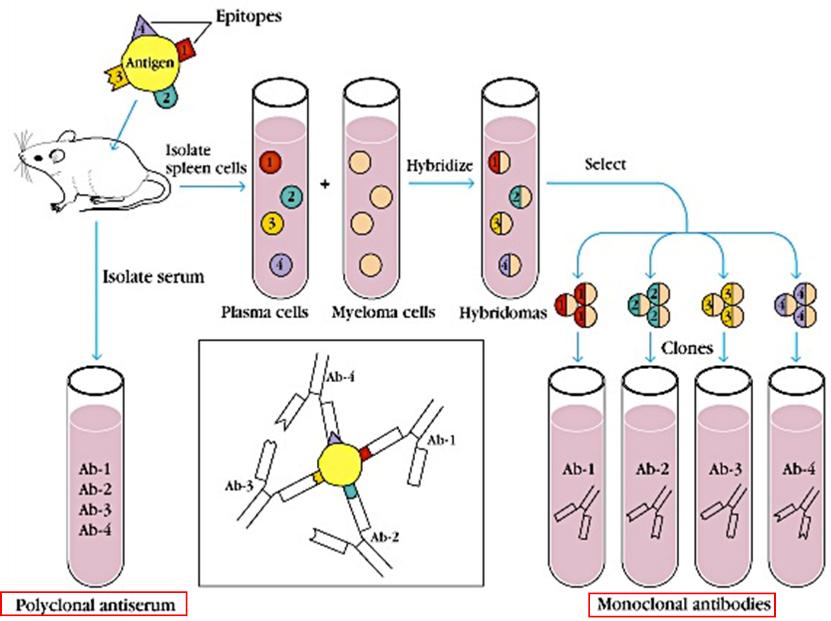
\includegraphics[width=0.60\textwidth]{img/27_ibridi_anticorpi.png}
  \caption{Immunizzazione per produzione di Ab}
\end{wrapfigure}

L’antigene con cui si immunizza il topo potrà essere una cellula intera, una membrana, un microorganismo. L'immunizzazione è facilitata tramite l'utilizzo di alcuni adiuvanti. Si fa una titolazione dell’anticorpo presente nel siero e poi si preleva la milza dopo due settimane.

Le cellule di mieloma (cellule tumorali) utilizzate per la fusione non devono solo essere immortali ma anche presentare la mutazione \textbf{HGPRT-} (mancano dell’enzima HGPRT). Questo enzima è normalmente responsabile della capacità della cellula di \emph{prelevare l’8-azaguanina}, un analogo della guanina e un potente mutageno citotossico, dal terreno di crescita. Questa caratteristica serve per selezionare le cellule ibride.

Il terreno di selezione utilizzato è il \textbf{terreno HAT} sul quale sopravvivono solo le cellule HGPRT+.\\
Perché le cellule HGPRT- muoiono? Perché il terreno HAT contiene un \textbf{inibitore della sintesi endogena dei nucleotidi}. 

HAT sta per:
\begin{itemize}
\item \textbf{hipoxantina}, un precursore delle purine
\item \textbf{aminopterina} (o \textbf{ametopterina}), un inibitore dell'enzima DHFR (deidrofolato reduttasi). Questo è un enzima essenziale per la via di sintesi endogena delle basi e dunque del DNA.\\
Questa è la stessa molecola utilizzata per il \textbf{metotrexato} o metotrexate, uno dei più diffusi agenti antiblastici (utilizzata come agente antitumorale soprattutto per la cura di leucemie e linfomi proprio perchè blocca la crescita delle cellule inibendone la sintesi del DNA, è una molecola molto usata nella chemioterapia)
\item \textbf{timidina}, un precursore delle pirimidine; 
\end{itemize}

A causa della presenza dell'aminopterina le cellule seminate su terreno HAT devono essere capaci di prelevare i precursori nucleotidici dal terreno. Le cellule di mieloma tuttavia, a causa della mutazione HGPRT-, non sono capaci di prelevare dal terreno le basi puriniche. Questa selezione può essere fatta anche mutando l'enzima TK (responsabile del prelievo delle basi pirimidiniche dal terreno).\\
Tramite questo terreno posso dunque eliminare le cellule di mieloma che non si sono fuse, mentre quelle che si saranno fuse formando l’ibridoma avranno per complementazione il gene HGPRT della cellula donatrice della milza, e saranno quindi capaci di crescere.

Perciò, inibendo l'enzima DHFR tramite l'aminopterina, non avviene la sintesi de novo delle basi. L’enzima DHFR infatti, si trova a monte di una serie di reazioni che portano alla formazione dell’\textbf{acido N5, N10 metilen-tetraidrofolico}, che è il maggior donatore di metili per la formazione della desossitimidina-monofosfato, uno dei precursori nucleosidici per la sintesi del DNA.

A causa del blocco della sintesi endogena del DNA viene utilizzata la via di salvataggio per la quale sono indispensabili due enzimi: la \textbf{timidina chinasi (TK)} per l’uptake delle pirimidine e l’\textbf{enzima ipoxantina-guanina-fosfo-ribosil-transferasi (HGPRT)} per l’uptake delle purine.

Ovviamente non si formeranno solo ibridi milza-mieloma ma anche ibridi omocellulari milza-milza, i quali però moriranno in quanto cellule primarie non immortali.

I cloni possono essere espansi anche nel topo, dove produrranno tumori ascitici portando a un alto titolo anticorpale (oggi non si fa più in vivo, vengono usati dei fermentatori).

\begin{figure}[h!]
\centering
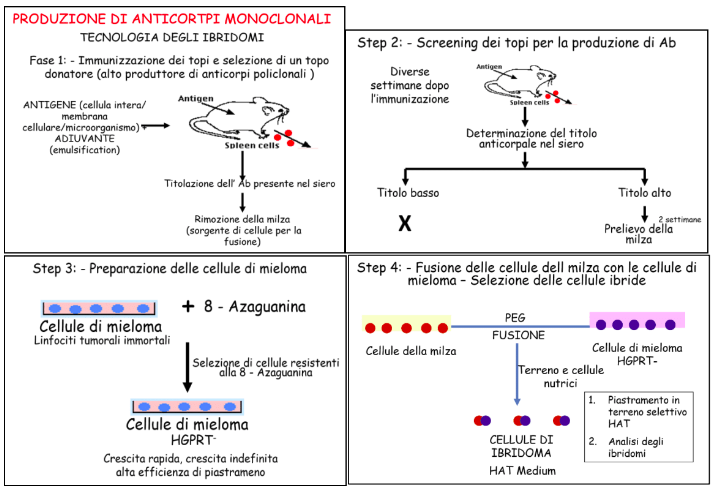
\includegraphics[scale=0.65]{img/28_anticorpi_monoclonali.png}
\caption{Preparazione anticorpi monoclonali in ibridi intraspecifici}
\label{}
\end{figure}

\subsubsection{Gli anticorpi umanizzati}
Per la terapia dei tumori si utilizza la cellula tumorale per immunizzare il topo cosicchè vengano produtti gli Ab con l'antigene tumorale specifico del paziente. 
In questo modo può essere attivata la risposta immunitaria contro la cellula tumorale richiamando le cellule NK, o associando all’anticorpo delle molecole terapeutiche.

È evidente che se lo scopo è terapeutico sarà necessario produrre anticorpi monoclonali umani e non più murini, i quali ovviamente non possono essere prodotti immunzzando un essere umano. Per questa ragione si producono gli \emph{``anticorpi umanizzati''}.\\
Se si somministra a un essere umano un Ab prodotto in una cellula animale diversa questo viene trattato come non-self e contro di esso si scatena una risposta immunitaria.
Nel caso della terapia tumorale però si vuole cercare di far passare anticorpi prodotti in una certa cellula come cellule self.

\begin{wrapfigure}{r}{0.70\textwidth}
    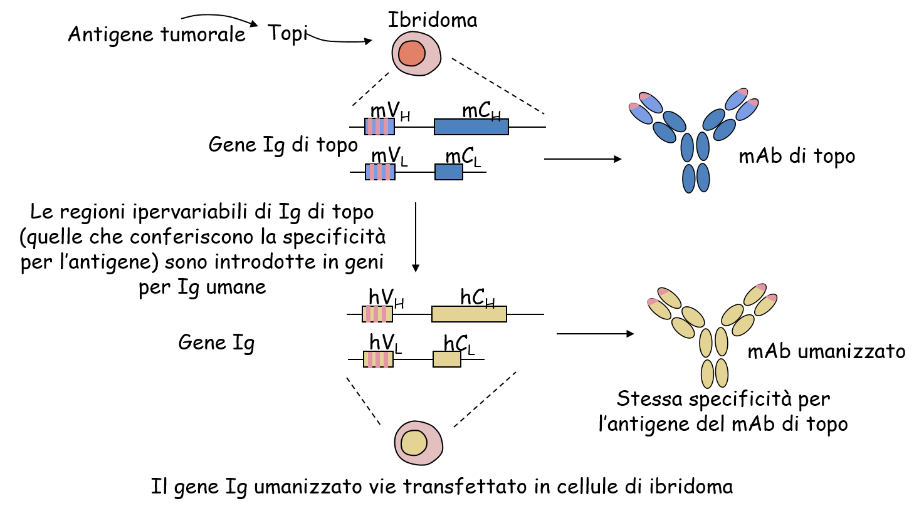
\includegraphics[width=0.7\textwidth]{img/30_ig_umanizzate.png}
  \caption{}
\end{wrapfigure}

Le difficoltà tecniche per produrre in vitro anticorpi umani da utilizzare per la terapia sono tante: non ci sono linee di mieloma adeguate, le cellule B umane possono essere immortalizzate ma perdono la capacità di produrre anticorpi (ovviamente non posso fare un trattamento in vivo ma devo trattare colture cellulari e la coltura cellulare non produce anticorpi a lungo termine) e inoltre è difficile ottenere cellule B umane attivate dall’antigene.

Per questa ragione non si agisce manipolando direttamente gli anticorpi ma producendo degli \textbf{anticorpi ibridi umanizzati}.
Per farli si modifica geneticamente il DNA di topo in modo che le cellule murine sintetizzino anticorpi con le \textbf{porzioni variabili murine} e le \textbf{porzioni costanti umane}.
La \emph{porzione variabile} è quella che riconosce l’anticorpo specifico, mentre la \emph{porzione costante} è quella che verrebbe riconosciuta come non self.

\begin{wrapfigure}{r}{0.50\textwidth}
    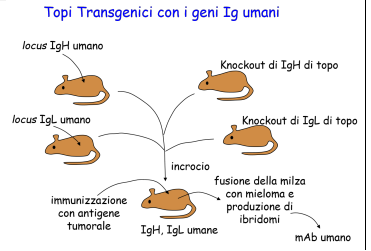
\includegraphics[width=0.50\textwidth]{img/31_topi_transgenici.png}
  \caption{}
\end{wrapfigure}

Anticorpi monoclonali umani si possono dunque ottenere producendo topi transgenici nei quali i geni che codificano le catene leggere e pesanti delle Ig di topo sono stati inattivati e sono stati introdotti al loro posto dei geni che codificano le catene leggere e pesanti umane.
In questo modo si ottiene un gene che codifica un anticorpo specifico, ma con un impianto anticorpale da Ig umana.

Naturalmente in questo processo la cosa più complicata è fare la modificazione genetica della cellula ricevente che verrà utilizzata per la produzione degli Ab umanizzati.
La differenza in questo approccio rispetto a quello visto prima è che nel primo lavoro veniva modificata la cellula dell’ibridoma lavorando in coltura cellulare, mentre in questo caso vengono costruiti dei topi transgenici capaci di produrre già Ig umanizzate.

\subsubsection{RICAPITOLANDO} 
Gli ibridi intraspecifici:
\begin{enumerate}
\item hanno cariotipo tetraploide
\item sono stabili in coltura
\item sono usati per:

	\begin{enumerate}
		\item studio dei rapporti di dominanza tra geni
		\item test di complementazione*
        \item studio dei meccanismi di regolazione dell’espressione genica 
        \item produzione di anticorpi monoclonali
        \end{enumerate}
\end{enumerate}

\textbf{*Test di complementazione}

Il test di Complementazione viene effettuato incrociando fra loro individui che presentano mutazioni le quali danno luogo allo stesso fenotipo. I geni, infatti, regolano singoli eventi di una catena metabolica, per cui la presenza di un fenotipo mutato può essere causata da una mutazione su uno qualsiasi dei geni che appartengono alla catena metabolica che risulta essere mutata.
Il test della complementazione permette di evidenziare se due individui o due cellule che presentano la stessa mutazione fenotipica abbiano subito una mutazione sullo stesso gene o su geni diversi.
Nell’incrocio, infatti, se le mutazioni sono su geni differenti si ottiene un fenotipo non mutato e le due mutazioni si dice che “complementano”; viceversa se esse sono sullo stesso gene, il fenotipo rimane mutato e le mutazioni “non complementano” proprio perché riguardano il medesimo gene e di conseguenza il medesimo enzima.
Nel test di complementazione vengono effettuate due prove: il test “Trans” in cui una mutazione si trova su un cromosoma e una sull’altro, ed il test “cis” in cui entrambe le mutazioni sono su un cromosoma mentre l’altro non presenta geni mutati. 
Se nel test “trans” le mutazioni complementano, ristabiliranno il fenotipo normale e questo significa che appartengono a geni diversi. Ciò però non è sufficiente, infatti la mutazione di un sito potrebbe interferire con l’espressione corretta dell’altro, perciò viene effettuato anche il test “cis”. Se in questo si presenta il fenotipo normale si può escludere l’ipotesi dell’inibizione del gene normale da parte di quello mutato e si può concludere che le mutazioni in questione appartengono a due geni diversi.
Tale test, detto anche “test cis-trans”, ha dato origine anche al termine di “cistrone”.

\subsection{Gli ibridi interspecifici}
A differenza degli ibridi intraspecifici, gli ibridi interspecifici vengono utilizzati per la localizzazione genica.
Questi ibridi vengono prodotti fondendo cellule in coltura provenienti da organismi di specie diverse.

Una caratteristica degli \emph{ibridi intraspecifici} è quella di essere delle cellule tetraploidi in cui coesistono i due cariotipi delle cellule parentali e, per complementazione genetica, dovrebbero essere espressi tutti i caratteri dell’una e dell’altra cellula (a meno che non ci siano dei fenomeni di repressione genica o di altre interazioni tra i genomi delle due cellule). 
Abbiamo visto che normalmente questi ibridi, in coltura, mantengono la condizione di tetraploidia e di espressione a lungo termine di tutti i marcatori che sono di interesse quando si produce l’ibrido. 
Gli ibridomi intraspecifici hanno anche questo grosso vantaggio: rispetto all’anticorpo policlonale prodotto nell’animale (e quindi presentante un’enorme variabilità), nel caso degli ibridomi abbiamo la produzione di anticorpi monoclonali (sono linee cellulari selezionate, quindi ci sarà uniformità nelle proteine prodotte e rilasciate nel terreno di coltura). Queste sono linee cellulari che vengono selezionate e poi stabilizzate in vitro, quindi a lungo termine sono molto stabili.

Nel caso degli \textbf{ibridi interspecifici} invece vengono fuse cellule diverse con caratteristiche molto diverse, fosse anche solo per la morfologia (organizzazione del citoscheletro). Ad esempio si possono fondere cellule che normalmente crescono in sospensione con cellule che crescono su un supporto solido, ma queste cellule hanno anche cromosomi e cariotipi diversi.
Le cellule che vengono fuse possono essere più o meno lontane dal punto di vista della specie di origine, ma generalmente all’inizio presentano tutte un \emph{cariotipo iperploide} (più di 2n), \emph{ipotetraploide} (meno di 4n) o \emph{ipertetraploide} (più di 4n).

Normalmente una delle due specie risulta essere prevalente sull’altra, ma questo varia sia al variare delle specie che al variare delle linee cellulari. Ad esempio nell’ibrido più comune, quello tra cellule di roditore e cellule umane, a prevalere sono normalmente le cellule di roditore, tuttavia non è sempre così e a fare la differenza sono le linee cellulari coinvolte.\\
Durante il processo di fusione delle due cellule normalmente si ha anche la fusione di più nuclei della cellula prevalente, contro un solo nucleo della cellula più debole. In generale dunque le cellule non sono perfettamente tetraploidi poichè il loro cariotipo non è dato dalla somma esatta del numero cromosomico di una e dell’altra specie, ma in generale hanno numeri cromosomici molto variabili e molto alti, quindi spesso sono ipertetraploidi o iperdiploidi (hanno 2 cariotipi di una delle due cellule parentali e un cariotipo dell’altra).

In ogni caso, a prescindere da quello che succede immediatamente dopo la fusione, bisogna ricordare che anche qui all’inizio si forma una cellula in cui vengono messi in comune i citoplasmi e che quindi sarà un \emph{eterocarionte} che conterrà o 2 nuclei (uno di un parentale e uno dell’altro) o 3 nuclei (2 di un parentale e 1 dell’altro). Inoltre, anche dopo che si sarà formato il \emph{sincarionte} (cioè dopo che si saranno fusi anche i nuclei), le cellule non saranno stabili in coltura perché tenderanno a ripristinare una condizione il più possibile vicina alla condizione normale di una delle due cellule parentali (quella appunto che ha l’impianto vincente).

Da cosa dipende il prevalere di una cellula sull’altra?\\ Fondamentalmente questo è un problema relativo alla ``forza'', ovvero alla capacità di reclutare un cinetocore funzionante che sia in grado di interagire con le fibre del fuso dei centromeri di una specie rispetto a quelli dell’altra. C’è una sorta di competizione fra centromeri delle due specie: i centromeri della specie vincente sono più forti, cioè reclutano un cinetocore più affine alle fibre del fuso, e per questo segregano correttamente. Al contrario, i centromeri dei cromosomi della specie svantaggiata hanno una minore affinità per le fibre del fuso, una minore capacità di reclutare un cinetocore funzionante e quindi segregano meno bene e vengono persi.

Il \emph{``selettivamente''} si riferisce alla unidirezionalità della perdita cromosomica, cioè vengono persi i cromosomi di una sola delle due specie, ma non esiste selettività per il tipo di cromosomi persi. La perdita è unidirezionale ma \emph{casuale}.


\textbf{RICAPITOLANDO}\\
Le caratteristiche degli ibridi interspecifici sono:
\begin{enumerate}
\item cariotipo iperdiploide, ipotetraploide, ipertetraploide
\item instabili in coltura
\item tendono a ripristinare la costituzione cromosomica di una delle specie parentali
\item perdono selettivamente i cromosomi di una delle specie parentali
\item utilizzati per:
	\begin{enumerate}
		\item studi di complementazione
        \item analisi di rapporti di dominanza
        \item studio della regolazione dell’espressione genica
        \item localizzazione genica
	\end{enumerate}
\end{enumerate}


Perché queste caratteristiche sono utili per la localizzazione dei geni sui cromosomi?
Supponiamo di voler localizzare su quale cromosoma si trova il gene che codifica per una certa proteina umana: innanzitutto viene fatto un estratto delle proteina dalla cellula ibrida e viene identificata la presenza della proteina di interesse. Ovviamente, essendoci una grossa omologia tra il genoma del topo e quello umano, avremo la stessa proteina sia nella forma umana che in quella murina e dovremo essere in grado di distinguerle. Generalmente queste due proteine, benchè simili, presentano una migrazione elettroforetica diversa. Oggi inoltre è anche possibile cercare la presenza di una specifica sequenza di DNA tramite PCR (anche piccole differenze vengono identificate in questo modo).

Se ad essere prevalente è l’assetto cellulare murino allora la proteina di topo sarà sempre presente (perché in questo caso vengono mantenuti tutti i cromosomi del topo), mentre la banda relativa alla proteina umana o l’amplificato di PCR ci sarà esclusivamente se tra i cromosomi conservati nella cellula ibrida c’è il cromosoma umano su cui è localizzato il gene che codifica per quella proteina.\\
A questo punto, se ho una serie di ibridi che contengono diversi cromosomi umani, posso costruire un pannello completo costituito da tanti cloni ibridi, ciascuno dei quali contiene una diversa combinazione di cromosomi umani. In questo modo per ogni cromosoma avrò una serie di ibridi contenenti quel cromosoma e una serie di ibridi che invece non lo contengono.

A questo punto localizzare il gene è banale: se io in tutti gli ibridi che hanno un particolare cromosoma identifico il prodotto proteico umano, mentre in tutti gli ibridi che mancano di quel cromosoma non identifico il prodotto proteico umano, è evidente che localizzo il gene specifico per quella proteina sul cromosoma che è sempre presente negli ibridi che la esprimono e che è sempre assente negli ibridi che non la esprimono.\\
È dunque l’\textbf{instabilità cromosomica} la caratteristica fondamentale per effettuare la localizzazione genica tramite ibridi interspecifici.

Per cosa vengono usati gli ibridi interspecifici?\\
Possono essere usati per diverse analisi di rapporti di dominanza tra geni diversi, o fra elementi regolativi e i geni da questi regolati. Ma soprattutto sono usati per la localizzazione genica.

La localizzazione genica attraverso questi ibridi oggi riesce ad arrivare ad una risoluzione che si avvicina al sequenziamento: arriviamo alla localizzazione specifica di un gene in termini di poche centinaia di pb sul genoma dell’organismo che ci interessa. Tutto questo si fa con delle tecniche di tipo citogenetico, che prevedono cioè analisi al microscopio.

Il metodo più utilizzato è quello della \textbf{``perdita cromosomica''}, ma esistono anche dei metodi alternativi quali:
\begin{itemize}
\item fusione con microcellule: per velocizzare la perdita cromosomica anziché fondere con cellule intere si utilizzano porzioni di cellule (microcellule)
\item trasferimento di singoli cromosomi (tecnica poco efficiente)
\item ibridi ridotti per irraggiamento: consentono di ottenere un mappaggio fisico con una risoluzione molecolare, cioè con poche paia di basi (si parla di Radiation Hybrids, o RH).
\end{itemize}

Nel caso della localizzazione genica per perdita cromosomica, gli ibridi più usati sono sempre stati quelli uomo-roditore.\\
In generale le cellule umane sono cellule primarie (non immortali), di solito \emph{fibroblasti} ottenuti tramite espianto di una porzione di circa 1 mm/quadro di tessuto sottocutaneo da un paziente (i fibroblasti sono tra le cellule umane che, se cresciute su supporto solido, vanno incontro a fusione più facilmente), mentre più raramente si tratta di linfociti da sangue periferico. Spesso è necessario prelevare queste cellule dal paziente, quindi non saranno linee cellulari immortalizzate ma semplicemente cellule ottenute da prelievi di sangue periferico o di altri tessuti, o espianti cutanei. 
Queste cellule umane dovrebbero essere normali (non mutanti).

Per le cellule di topo invece il vantaggio è che esistono in commercio numerose colture cellulari stabilizzate; inoltre le cellule di topo in coltura si trasformano molto facilmente (è facile avere delle linee immortali che crescono facilmente in laboratorio), sono molto comode da manipolare e inoltre sono molto stabili dal punto di vista delle caratteristiche biochimiche e del cariotipo.\\
Le cellule più comode di tutte sono quelle di criceto, e la linea di cellulare di criceto per eccellenza, è quella delle \textbf{CHO} (Chinese Hamster Ovary). Questa è una linea cellulare che cresce molto bene in coltura e in questo caso i cromosomi sono molto riarrangiati rispetto a quelli del criceto cinese in natura: sono pochi cromosomi, allungati, molto facili da identificare e bandeggiare.\\
Nell’ibrido uomo-topo la perdita dei cromosomi umani è piuttosto lenta, mentre è molto più rapida negli ibridi uomo-criceto (è più utile usare gli ibridi uomo-CHO).

Una delle linee immortalizzate più usate in laboratorio è quella delle \textbf{cellule Hela}. Questa è una linea umana stabilizzata derivate dal cancro di Henrietta Lacks. Queste linee circolano da 40-50 anni nei laboratori di tutto il mondo e per questo cellule Hela coltivate in laboratori diversi hanno poco in comune: queste cellule si sono talmente adattate alle condizioni di coltura da presentare una serie di varianti, non solo cromosomiche (perché hanno cariotipi aberranti) ma anche genomiche. Quindi queste linee cellulari sono comodissime perché capaci di crescere molto facilmente, ma sono anche molto pericolose da coltivare perché sono altamente contaminanti: la contaminazione batterica o di lieviti è meno grave della contaminazione di una linea cellulare da parte di un’altra linea cellulare, perché è più difficile accorgersene e liberarsene.\\
Le linee di criceto hanno invece il grosso vantaggio che i cromosomi di criceto sono talmente diversi da quelli di topo, di ratto e umani che la contaminazione la si identifica facilmente, semplicemente facendo un’analisi cromosomica.

Normalmente negli ibridi uomo-roditore vengono persi selettivamente i cromosomi umani, ed è per questo che sono utili per localizzare i geni sui cromosomi umani.\\
La perdita è casuale e dopo un numero variabile (a seconda delle cellule parentali utilizzate) di generazioni in coltura l’ibrido si assesta in una condizione di equilibrio in cui vengono ritenuti pochi cromosomi (nei casi ideali viene mantenuto un solo cromosoma umano, ma più di frequente vengono mantenuti 2-3-5 cromosomi umani, e il cariotipo completo o addirittura 2 cariotipi completi di roditore).\\
Quindi dopo un certo tempo in coltura, che varia a seconda degli ibridi che io ho fatto, avrò delle colture stabili in cui le cellule contengono numeri diversi e una combinazione diversa di cromosomi umani.
È una coltura mista di cellule che dovranno essere clonate.
 
\textbf{Ricorda}: si definisce \textbf{``clone''} è \emph{una popolazione di cellule derivate da una sola cellula}. Per ottenerle o si semina in piastra da 96 pozzetti oppure si seminano, molto diluite, in piastre petri. Si verifica che ogni popolazione effettivamente derivi da una singola cellula (e ciò si fa al microscopio) e poi, con tecniche diverse, si isolano i diversi cloni. A questo punto avrò una popolazione di cloni ibridi, tutti diversi tra loro per contenuto di cromosomi umani residui.

\begin{wrapfigure}{r}{0.45\textwidth}
\centering
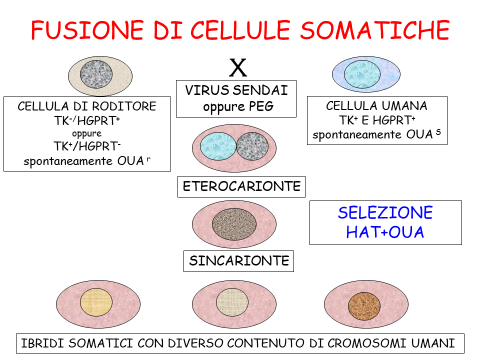
\includegraphics[width=0.45\textwidth]{img/32_fusione_cellule_somatiche.png}
  \caption{}
\end{wrapfigure}

Come agente fusogeno oggi non si usa più il virus Sendai, ma si usa un polimero ad alto peso molecolare, il \textbf{polietilenglicole (PEG)}. Il PM del PEG può essere variato a seconda delle cellule che devo fondere, in quanto devo valutare sia l’efficienza (più alto è il peso molecolare maggiore è l’efficienza a formare ponti citoplasmatici) che la citotossicità.

Il PEG è affine alla membrana cellulare e in questo modo crea dei ponti citoplasmatici originando l’eterodicarionte.\\
L'utilizzo del PEG è essenziale in quanto eventi di fusione spontanea tra cellule di mammifero sono rarissimi e praticamente non si riescono a selezionare le cellule ibride se non uso un induttore della fusione. 

Ma come si fanno fondere le cellule?\\
Semino in una piastra, in un rapporto 1:1, le cellule parentali dei due tipi. Perché le cellule si fondano devono essere vicine, ma pur avendo diluito perfettamente le cellule e sospendendole accuratamente, una volta piastrate non avrò sempre vicine cellule umane con cellule di roditore, ma si formeranno 3 tipi di ibridi: 
\begin{enumerate}
\item ibridi uomo-uomo
\item roditore-roditore
\item uomo-roditore.
\end{enumerate}

Inoltre una \% di cellule non si fonderà per niente, e quindi avrò anche delle cellule parentali (sia umane che murine). Per questa ragione è necessario avere un sistema di selezione che mi permetta di far sopravvivere solo gli ibridi che mi interessano, di eliminare quelli che non servono e di eliminare le cellule parentali. Quello che si usa è il sistema HAT.

I geni di interesse per questo sistema sono il TK (timidina chinasi) e HGPRT (ipoxantina-guanina-fosforibosiltransferasi), 2 geni hous-keeping.\\
Il gene TK è necessario per modificare le basi pirimidiniche, mentre il gene HGPRT è necessario per modificare le basi puriniche. Questa modificazione prevede l’aggiunta di un residuo alle basi così da poter prelevare dal mezzo di crescita i precursori pirimidinici e purinici.\\
La presenza di questi due geni permette quindi alla cellula, se si trova in un terreno contenente dei precursori, di modificarli per poterli poi metabolizzare per la sintesi del DNA (questo normalmente non è indispensabile perché tutte le cellule hanno la capacità di fare una sintesi endogena delle pirimidine e delle purine).

Le linee cellulari di roditore vengono selezionate così da essere mutanti TK- o HGPRT-; non è necessario che le cellule siano mutanti per entrambi i geni in quanto le vie di sintesi di purine e pirimidine sono dipendenti l’una dall’altra (quindi se blocco una delle 2 vie blocco anche l’altra e se ne attivo una, attivo anche l’altra).\\
Per la selezione di queste cellule si mette nel terreno di coltura un agente che sia analogo di una purina o di una pirimidina e che, se prelevato dal mezzo, risulta molto tossico per la cellula. Per questa ragione le cellule, per poter sopravvivere in questo terreno selettivo, dovranno risultare incapaci di prelevarlo dal mezzo di crescita.\\
Per selezionare cellule \textbf{TK-} si usa la \textbf{bromodesossiuridina (BUdr)}, un mutageno ad alte dosi, analogo delle pirimidine: metto le cellule in un terreno contenente BUdr e seleziono i cloni resistenti, capaci di sopravvivere (essendo TK- non raccolgono BUdr dal mezzo). Se sono TK- ovviamente saranno HGPRT+.
Per selezionare le cellule \textbf{HGPRT-} invece si usa la \textbf{6-tioguanina} (o anche l’\emph{8-azacitidina}), un analogo altamente mutageno delle purine.

Queste cellule mutate per TK e HGPRT, se si blocca anche la via endogena di sintesi di purine e pirimidine, non potendo fare l'uptake dei precursori andranno incontro a morte.

A questo punto sarà possibile selezionare le cellule ibride grazie al fenomeno della \textbf{complementazione genetica}: solo gli ibridi in cui i due nuclei sono derivati da un donatore murino e un donatore umano saranno sia TK+ che HGPRT+, in quanto avranno acquisito il gene TK e HGPRT wild type dalla cellula umana.

Per selezionare gli ibridi viene utilizzato nuovamente il terreno selettivo HAT. In un terreno di questo tipo, siccome è bloccata la via endogena di sintesi del DNA, sopravvivono solo le cellule capaci di attivare la via di salvataggio, ovvero quella che prevede che gli enzimi TK e HGPRT funzionino. È evidente che in questo terreno selettivo moriranno le cellule che sono TK- o HGPRT-, eliminando così i parentali di topo e tutti gli ibridi topo-topo. 
Sarà però ancora necessario liberarsi degli ibridi uomo-uomo e delle cellule parentali umane.

Per eliminare le cellule umane si sfrutta una caratteristica tipica delle cellule di roditore rispetto alle cellule umane: esiste una dose soglia alla \textbf{ouabanina} (potente veleno della pompa Na/K che ad alte concentrazioni ammazza le cellule) alla quale sono spontaneamente resistenti le cellule di roditore e sensibili le cellule umane. Ecco allora che se uso un \textbf{terreno HAT+ouabanina}, posso eliminare anche tutte le cellule umane e gli ibridi uomo-uomo.
A questo punto le uniche cellule in grado di sopravvivere saranno gli ibridi interspecifici.

Dopo la selezione in HAT avrò una popolazione eterogenea di cellule che, quando clonate, mi daranno un numero \emph{N} di cloni ibridi ognuno dei quali avrà perso selettivamente ma casualmente cromosomi umani, e presenterà dunque combinazioni di cromosomi diverse. 

Questa è la conclusione del protoccolo per la produzione di ibridi interspecifici per studi di localizzazione genica.

Avevamo già detto all'inizio che gli ibridi interspecifici sono cellule non stabili in cui uno dei due assetti cromosomici risulta essere più efficiente nel reclutamento delle proteine necessarie per la formazione del cinetocore, e che è proprio questa caratteristica a causare la perdita selettiva dei cromosomi di una delle due specie (quelli di uomo nel caso di ibridi topo-uomo). Abbiamo anche appena detto che a permettere la sopravvivenza di questi ibridi è la presenza dei geni TK e HGPRT umani. Da qui non è difficile capire come, se si mantiene la pressione selettiva continuanto a crescere i nostri cloni ibridi su terreno selettivo, si arriverà ad avere cellule che contengono solo i cromosomi umani che portano questi due cromosomi indispensabili, mentre tutte le cellule che hanno perso l'uno o l'altro saranno morte (N.B. l'assetto cromosomico murino viene sempre mantenuto).

Ammettiamo di partire da cellule parentali di roditore HGPRT-: in genere il gene \textbf{HGPRT} si trova sul \textbf{cromosoma X} nell’uomo, quindi verranno selezionati tutti quegli ibridi che hanno mantenuto il cromosoma X umano. Di conseguenza avrò un pannello di ibridi più o meno completo ma, finché mantengo la pressione selettiva, per forza di cose tra i cromosomi mantenuti nell'ibrido ci sarà il cromosoma X. In questo modo è particolarmente facile ottenere degli ibridi monocromosomici, basta mantenere la pressione selettiva per molto tempo. Per quanto riguarda il gene \textbf{TK} invece, questo è localizzato sul \textbf{cromosoma 17}, sarà dunque facile ottenere degli ibridi monocromosomici che conterranno il cromosoma 17.
 
Tuttavi per i nostri scopi l’ideale sarebbe poter avere ibridi monocromosomici per ognuno dei nostri cromosomi, dunque 24 ibridi diversi (22 autosomi, + l’X e l’Y). Se un ibrido monocromosomico esprime un certo gene umano questo gene non potrà che essere presente su quel cromosoma.
Tuttavia per selezionare gli ibridi avremo bisogno di marcatori specifici che non sono naturalmente presenti (quelli naturalmente presenti sono TK sul Ch.17 e HGPRT sul Ch.X).

Uno dei metodi utilizzati per inserire dei marcatori selettivi specifici che permettano di selezionare cromosomi che non siano il 17 e l'X è quello della \textbf{trasformazione shot-gun}. Uno dei marcatori più utilizzati è ad esempio il \textbf{gene Neo} che, nelle cellule di mammifero, \textbf{conferisce resistenza a G418}, un analogo della \textbf{neomicina}. Le cellule che contengono questo gene, se coltivate su un terreno contenente G418, sopravvivono, mentre le cellule che non lo contengono muoiono. 

Si parla di trasformazione shot-gun perchè l'integrazione del gene nel DNA eucariotico sarà casuale.

Quando si fa una trasformazione semplice in cellule umane inserendo un plasmide possono succedere due cose:
\begin{enumerate}
\item il DNA, una volta entrato nel nucleo, può essere riconosciuto come estraneo, digerito dagli enzimi di restrizione ed eliminato;
\item può essere integrato in maniera \underline{casuale} all'interno del genoma della cellula ospite.
\end{enumerate}

Questo metodo di integrazione viene detto \emph{``a pioggi''} proprio per la componente della casualità.

Ovviamente, una volta fatta la trasformazione, molte cellule potranno presentare la resistenza, tuttavia questa può essere una resistenza a breve termine dovuta semplicemente alla presenza del plasmide e per questo è necessario assicurarsi che la resistenza venga mantenuta anche \emph{a lungo termine} così da avere la certezza che il gene sia stato integrato in uno dei cromosomi.

Questo tipo di integrazione, proprio perchè casuale, mi permetterà di avere degli ibridomi che avranno integrato il gene marcatore ognuno su un cromosoma diverso, il che mi permetterà in futuro di ottenere ibridi monocromosomici per ognuno dei diversi cromosomi.

A questo punto possono crosturire un pannello di ibridi, ognuno contenente combinazioni diverse di cromosomi (non faccio sempre l'ibrido monocromosomico perchè richiede molto tempo), che coprono tutto il genoma e che mi permettono di escludere o includere in diversi cloni ciascuno dei cromosomi umani.\\
Per capire meglio come funziona questo metodo consideriamo la figura \ref{localizzazione_genica}

\begin{figure}[htp]
\centering
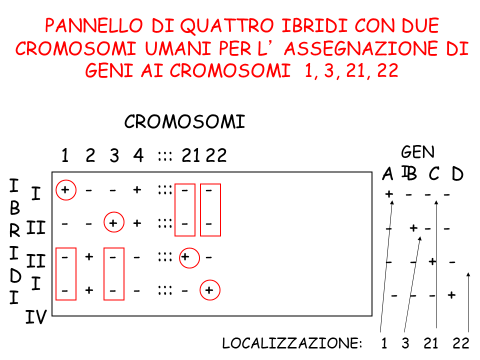
\includegraphics[scale=0.70]{img/33_localizzazione_genica.png}
\caption{Pannello per la localizzazione genica}
\label{localizzazione_genica}
\end{figure}

In questo esempio abbiamo solo 4 ibridi caratterizzati in cui:
\begin{itemize}
\item nel 1° ibrido: è presente il cromosoma 1, non ci sono il cromosoma 2 e 3 ed è presente il cromosoma 4, non sono presenti i cromosomi 21 e 22
\item il 2° ibrido per quanto riguarda il cromosoma 21 e 22 è assolutamente identico al 1°, quindi questi non mi permettono di discriminare tra il cromosoma 21 e il 22. In compenso è diverso dal 1° per quanto riguarda il cromosoma 1, che è presente nel 1° ibrido e non nel secondo, e il cromosoma 3 che è assente nel primo ibrido ed è presente nel secondo. Anche il cromosoma 4 è presene in entrambi gli ibridi quindi non posso discriminare
\item negli altri ibridi non posso discriminare tra il cromosoma 1 e il 3 perché i due ibridi mancano di questo cromosoma. In compenso l’ibrido 3 ha il cromosoma 21 e non il 22, e viceversa l’ibrido 4 ha il cromosoma 22 e non il 21.
\end{itemize}

Come faccio l’analisi?\\
Per ciascun ibrido devo stabilire la presenza/assenza del gene, della proteina o della sequenza di DNA che voglio identificare (posso identificare la sequenza di DNA identificandola con una sonda o amplificandola per PCR), dopodichè vado a vedere le concordanze, cioè quante volte c’è concordanza tra presenza del cromosoma e presenza del gene (e viceversa, cioè quante volte non c’è concordanza tra la presenza del cromosoma e la presenza del gene).\\
Andiamo a vedere i 4 diversi geni che qui sto indagando:
\begin{itemize}
\item il gene A è presente soltanto nel 1° ibrido quindi è evidente che, essendo il 1° ibrido l’unico ad avere il cromosoma 1, il gene A sarà localizzato sul cromosoma 1
\item il gene B è presente esclusivamente nel 2° ibrido e quindi non può che trovarsi sul cromosoma 3
\item il gene C si trova solo nel 3° ibrido, per cui si troverà sul cromosoma 21
\item il gene D, invece, si trova sul cromosoma 22. 
    \end{itemize}

Ovviamente questa è una situazione molto semplificata.

\textbf{Domanda alla prof:} \emph{``Nel caso in cui si ha amplificazione di un gene, o comunque il gene si trova su più cromosomi?''}\\
\textbf{Risposta:} ``Può succedere ma in generale lo si sa se si tratta di una famiglia multigenica. Nella maggior parte dei casi le famiglie multigeniche e anche le sequenze ripetute (se parliamo di sequenze codificanti per proteina), sono localizzate su un cromosoma.''

\textbf{Domanda alla prof:} \emph{``E se c’è una traslocazione?''}\\
\textbf{Risposta:} ``Lo si sa prima perché per prima cosa viene fatta una importante analisi citogenetica per caratterizzare gli ibridi, inoltre la linea parentale umana che si usa è una linea che è stata caratterizzata, per cui se c’è stata una traslocazione lo saprò e saprò anche dove è traslocato il segmento che mi interessa e da quale cromosoma proviene. Quindi la caratterizzazione citogenetica dettagliata della linea parentale che si usa è fondamentale.\\
Comunque si può sfruttare la traslocazione che separa un piccolo segmento cromosomico per fare una localizzazione regionale, per cui con un approccio come quello appena visto io stabilisco semplicemente che il gene si trova, per esempio, sul cromosoma 1, ma questo è un cromosoma enorme quindi in quale regione del cromosoma 1 si troverà? Per poter sapere qualcosa in più prendo dei fibroblasti di pazienti che hanno delle piccole traslocazioni, e in questo modo è come se io isolassi quel piccolo segmento del cromosoma 1, sfruttando il fatto che è traslocato. A questo punto se il mio gene di interesse è traslocato su un altro cromosoma umano isolerò un ibrido monocromosomico che contenga \emph{non il cromosoma 1} ma l’altro cromosoma su cui c’è il pezzetto di cromosoma 1 traslocato, dopodichè andrò a vedere se dove c’è la traslocazione c’è anche il gene. È un metodo macchinoso che veniva usato in passato, mentre ora ci sono delle tecniche molto più efficienti per fare la localizzazione regionale. Ovviamente non si può andare a caso, ma in generale si deve avere già qualche indicazione della localizzazione regionale, che possono provenire per esempio da approcci di studi familiari: se è un gene malattia gli studi familiari mi dicono che c’è un marcatore anonimo che so essere localizzato in una certa regione del genoma e allora studio una particolare traslocazione di una specifica regione, dove so che c’è quel marcatore anonimo.

Qual è il vantaggio dell’ibrido somatico?
Per orientarmi uso un paziente che ha una traslocazione che coinvolge quella porzione che io so essere quella interessante perché ho un marcatore polimorfico che segrega con il gene malattia nelle famiglie.
Quindi produco l’ibrido somatico con quel pezzettino di cromosoma 1 (ad esempio), proprio quel pezzo traslocato su un altro cromosoma.
A questo punto, su questo ibrido, quando estraggo il DNA ho un arricchimento enorme di geni, e solo di quelli in cui c’è per forza dentro il gene malattia, perché ho un segmentino che contiene il gene malattia e il marcatore polimorfico molto molto vicino. Questo è un vantaggio enorme perché a questo punto posso sequenziare quel pezzettino del cromosoma 1 e identificare tutti i geni candidati, e cioè quei geni che codificano per una proteina ma soprattutto che sono mutati nei pazienti.
Questo è stato un approccio usato in alcuni casi per identificare i geni malattia, perché l’ibrido somatico mi dà il modo di avere, su un background di topo, soltanto quel segmentino umano in cui certamente c’è dentro il gene malattia, e quindi quando amplifico questo segmento, lo sequenzio e lo clono, ho la certezza che tra tutto quello che ho clonato ci sarà dentro il gene malattia, e quindi poi vedendo se è mutato nei pazienti lo identifico.
In passato questo approccio è stato usato per identificare geni importanti, come quello della fibrosi cistica, o anche per identificare il gene coinvolto nella sindrome dell'X fragile.\\
La localizzazione regionale si può fare sfruttando pazienti con riarrangiamenti cromosomici, una volta identificato il cromosoma su cui si trova il gene di interesse.

Quello che si fa sono delle \textbf{``Tabelle di Discordanza''}: si fanno delle tabelle di \emph{discordanza} e \emph{non di concordanza} in quanto è più facile avere dei \emph{falsi positivi} che dei falsi negativi (è una ragione pratica dovuta all’errore sperimentale).

\begin{wrapfigure}{r}{0.7\textwidth}
    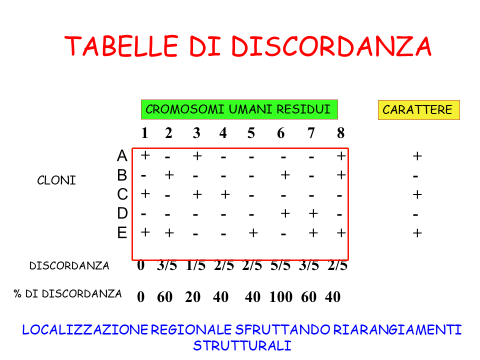
\includegraphics[width=0.7\textwidth]{img/34_tabelle_discordanza.png}
  \caption{Tavella di discordanza}
\end{wrapfigure}

Anche qui si considera un pannello con 5 cloni e solo 8 dei 24 cromosomi umani.\\
Per ogni ibrido considererò la presenza/assenza di ogni cromosoma preso in considerazione e la presenza/assenza del carattere, dopodichè per ogni \underline{cromosoma} conterò il numero di discordanze, ovvero quante volte ol cromosoma è presente mentre il carattere è assente e viceversa (+/- o -/+). Avrò invece concordanza quando sia il cromosoma che il carattere saranno presenti o assenti (+/+ o -/-).

Ovviamente il gene in analisi sarà presente sul cromosoma per il quale \textbf{la discordanza sarà 0} o molto vicina a 0 (in percentuale o in frazione) o, viceversa, \textbf{la concordanza sarà 100} (se è in percentuale o 1 se e in frazione).

\clearpage
Quindi per ogni cromosoma ci chiediamo: quanti cloni hanno il cromosoma 1? E dove è presente il carattere?
Facciamo questo per ogni cromosoma, poi riportiamo il valore di discordanza. Nel caso della nostra tabella l’unico cromosoma per cui c’era una percentuale di discordanza pari a 0 è il cromosoma 1, per cui è evidente che il gene che codifica per il carattere considerato si trova sul cromosoma 1.


\subsection{Gli ibridi ridotti per irragiamento (Radiation Hybrids - RH)}

Tramite l'utilizzo delle tabelle di discordanza si ha una localizzazione abbastanza approssimativa dei geni in quanto possiamo sì individuare su \emph{quale} cromosoma il gene sia localizzato, ma i cromosomi sono entità molto grandi che possono andare, in base alla dimensione, da 5-6 Mb fino a 15-20 Mb.

La tecnica degli ibridi ridotti per irragiamento permette di arrivare a una risoluzione/localizzazione di livello molecolare, cioè molto vicina alla sequenza (poche decine di pb).

Il punto di partenza per ottenere degli ibridi ridotti per irraggiamento è quello di avere degli ibridi somatici monocromosomici tramite la tecnica della perdita cromosomica in ibridi interspecifici. 
Per poter ottenere ibridi monocromosomici per ogni cromosoma verrà fatta una trasformazione a pioggia che causerà l'integrazione casuale del gene Neo (è il più usato) conferendo così resistenza all'antibiotico G418 (analogo della neomicina efficiente nelle cellule di mammifero).

Dopo essersi assicurati che la resistenza antibiotica sia dovuta all'effettiva integrazione del gene del genoma che voglia studiare si avrà una popolazione di ibridi mista in cui ogni ibrido avrà integrato il gene in un sito diverso. 

La tecnica degli ibridi ridotti per irragiamento è una tecnica di confine tra l'\emph{approccio citologico/fisico} dell'ibridazione di cellule somatiche (è definito fisico perchè permette di sapere la posizione reale, la distanza fisica del gene rispetto ad altre sequenze), e l'\emph{approccio statistico/probabilistico} dell'analisi di linkage (è definito statistico perché viene calcolata la vicincanza tra due sequenze sulla base della probabilità che queste vengano separate da un evento di ricombinazione: una sequenza sarà più vicina ad un’altra quanto minore è la frequenza di ricombinanti che ritrovo in una progenie).\\
Con la tecnica dell'irragiamento degli ibridi tuttavia a essere presa in considerazione non è la probabilità che due sequenze vengano separate da fenomeni di ricombinazione meiotica ma \emph{la distanza viene calcolata sulla base della probabilità che due marcatori vengano separati dalla rottura indotta dalla radiazione ionizzante.}

Questo viene fatto esponendo gli ibridi monocromosomici a radiazioni ionizzanti altamente clastogene (i.e. che inducono alterazioni nella struttura del cromosoma), tipicamente Raggi X. Più alta è la dose di raggi X, più piccoli saranno i frammenti in cui si spezzeranno i cromosomi della cellula irradiata.

Passiamo al protocollo:\\ 
il punto di partenza per questa tecnica sono:
\begin{itemize}
\item un \textbf{ibrido primario monocromosomico}
\item una cellula di roditore.
\end{itemize}

L’ibrido monocromosomico viene esposto a una dose di raggi X, scelta in base alle necessità, che riduce tutti i cromosomi dell’ibrido primario in frammenti tanto più piccoli quanto più alta è la dose di raggi X utilizzata.

Il fatto che gli ibridi primari, come conseguenza dell'irradiazione, oltre ad avere cromosomi spezzettati vadano incontro a morte cellulare non ci importa, in quanto questo non influenza la membrana e dunque la capacità del PEG di indurre fusione tra questa cellula e quella di roditore.

A questo punto l'ibrido secondario conterrà una popolazione di frammenti cromosomici umani e murini insieme a tutti i cromosomi di topo (N.B. la maggior parte dei frammenti di cromosomi saranno di topo in quanto l'ibrido primario conteneva \emph{un solo} cromosoma umano e l'intero assetto cromosomico murino). I frammenti cromosomici umani spezzettati però, a causa delle loro estremità libere, saranno estremamente instabili e reattivi e potranno andare incontro a due diversi destini:
\begin{enumerate}
\item potranno essere \textbf{degradati dalle esonucleasi nucleari}
\item potranno integrarsi a caso all'interno dei cromosomi della cellula ospite
\end{enumerate}

Questo destino riguarderà sia i frammenti murini che umani, ma ad interessarci saranno solo quelli umani.

A questo punto sarà necessario selezionare e clonare gli ibridi ottenuti e quello che si otterrà alla fine saranno tanti cloni diverdsi in cui, nei cromosomi murini integri di ognuno di essi, si saranno integrati in maniera causale frammenti cromosomici umani diversi.

In altre parole avrò una popolazione di ibridi secondari con diversi frammenti del cromosoma inizialmente presente nell’ibrido monocromosomico integrati nei cromosomi di topo.

Cose si procede per la localizzazione regionale?
Per la localizzazione verrà sfruttato un marcatore noto (questo può essere un gene malattia o un marcatore anonimo). Ora, grazie al completo sequenziamento del genoma umano, è possibile procurarsi delle sequenze note di DNA, generalmente clonate in BAC\textbf{*}, distribuite in maniera abbastanza uniforme lungo tutto il cromosoma umano dell'ibrido primario ed utilizzare queste come marcatori di riferimento.

\textbf{BAC (Bacterial Artificial Chromosome):} è un vettore articiale di DNA basato sul plasmide F isolato da E.coli. Si differenzia dai normali plasmidi in quanto è in grado di trasportare regioni di DNA di interesse molto più ampie, arrivando a tollerare inserti fino a 300 Kb (mediamente 100 Kb) rispetto alle 2-4 Kb che possono essere normalemnte inserite all'interno dei plasmidi.

A questo punto i singoli cloni vengono analizzati per la presenza contemporanea del gene di interesse e di uno di questi marcatori anonimi, scelti perché coprono tutto il cromosoma in analisi.\\
Alcuni di questi frammenti saranno molto lontani dal gene di interesse, perciò la probabilità che si trovino sullo stesso frammento presente in uno dei miei cloni (che, ricordiamo, contengono soltanto un frammentino del cromosoma) sarà molto bassa.\\
Quello che si fa è andare a contare, marcatore per marcatore, in quanti cloni è presente sia il marcatore che il gene di interesse: se i marcatori sono lontani dal gene non ci sarà praticamente nessun clone che conterrà sia il marcatore che il gene di interesse, mentre se il marcatore si trova vicino al gene la probabilità che questi siano stati separati dalla radiazione diminuirà e la probabilità di trovare dei cloni che contengono entrambi sarà maggiore.

Alla fine sarà possibile individuare, per un solo marcatore, un numero altissimo di cloni che contengono contemporaneamente il gene di interesse e il marcatore (di cui io conosco la posizione genomica). È evidente che se il numero di cloni in cui marcatore e gene sono contemporaneamente presenti è molto alto vuol dire che le due sequenze si trovano molto vicine (perché non sono mai state separate o sono state separate poche volte dalla rottura indotta da irraggiamento). 

Questo chiarisce perchè il metodo sia in parte definito di tipo statistico, perché conto i cloni e statisticamente una sequenza è tanto più vicina quanto meno è probabile che sia stata separata dal gene di interesse per un evento di rottura indotto da irraggiamento (invece nel caso di approccio genetico è la ricombinazione che separa le sequenze).

Questo approccio permette una risoluzione/localizzazione molto più elevata perchè non dipende dalla numerosità della progenie (come avviene nell'approccio genetico basato sulla ricombianzione meiotica), inoltre i frammenti scelti come marcatori che ricoprono tutto il cromosoma possono essere anche molto piccoli permettendomi di arrivare estremamente vicino al gene di interesse. Una volta arrivati così vicino al gene sarà possibile sequenziare quel segmento e, se nel caso questo sia un gene malattia, andare a verificare se è mutato nei pazienti e fare tutte le analisi del caso. 

La risoluzione di questa tecnica è sovrapponibile al mappaggio molecolare.

\textbf{Domanda}: \emph{Questa tecnica viene utilizzata per cercare un gene causativo di malattia?}\\
\textbf{Risposta della prof:} Considerato che ormai tutti i geni malattia sono sequenziati, ad oggi questi approcci vengono utilizzati per confermare dei mappaggi che vengono fatti sulla base dell’allineamento di Bac.

Come si costruisce un mappaggio completo di un genoma? Per costruire un mappaggio completo di un genoma fondamentalmente si allineano, per estremità condivise, degli enormi segmenti genomici clonati in Bac (150-200 Kb). Questi segmenti vengono allineati soltanto sulla base della corrispondenza/complementarietà delle estremità costruendo così dei grossi ``contigui'' (stiamo parlando di genomi di miliardi di pb quindi bisogna considerare pezzi grossi). Questi contigui sono costruiti su base statistica perché io non so esattamente cosa c’è in mezzo (in mezzo c’è un’enorme quantità di DNA genomico di cui io non so nulla se non che le estremità di questi segmenti sono complementari alle estremità dei segmenti successivi).\\
È evidente che le \emph{``mappe grezze''} dei genomi, cioè questi primi allineamenti di contigui, devono essere confermate segmento per segmento, e quindi questi approcci servono per avere delle conferme sperimentali di dati puramente deduttivi.
Molto spesso vengono fatte, per esempio, sulla base di note omologie di sequenze conservate nello stesso ordine e cioè in gruppi di linkage; ma non è detto che questi gruppi di linkage siano sempre conservati in organismi diversi, perciò per decodificare i genomi complessi e soprattutto per avere delle mappe fedeli bisogna usare dei metodi sperimentali e uno di questi è proprio l’uso dei Radiation Hybrids.

Comunque, almeno nell’uomo, la localizzazione e il sequenziamento dei geni malattia si conoscono già. Bisogna inoltre dire che nella maggior parte dei casi, le malattie non sono semplicemente dovute a mutazioni in singoli geni ma sono dovute anche a eventi epigenetici, come nel caso di alcuni tumori. Per esempio ci sono degli approcci di diagnosi precoce del tumore che vengono fatti grazie alla scoperta che ci sono dei non-coding RNA (i non-coding RNA sono molecole che regolano l’espressione genica), che sono marcatori tumorali perché regolano proprio l’espressione dell’oncogene, dell’oncosoppressore o di una sequenza coinvolta nello sviluppo del tumore.\\
Ecco allora che anche queste tecniche ad alta risoluzione possono servire per caratterizzare queste altre molecole che non sono correlate in maniera diretta al gene-malattia, perché non sono quelle che mutano nella malattia, ma la cui espressione altera l’espressione del gene-malattia. 
Poi ci sono altri casi: per esempio si è scoperto che ci sono delle regioni che contengono delle sequenze che variano per numero di copie, si chiamano Copy Number Variation (CNV), queste sequenze sono localizzate in zone particolari del genoma e si è visto che nella popolazione sono polimorfiche, ma si tratta di segmenti genomici enormi che variano per numero di copie.

Le Copy Number Variation hanno un impatto nell’espressività e nella penetranza di un sacco di malattie complesse. Queste nuove scoperte inducono a dissezionare il genoma in maniera sempre più specifica per capire come variano queste sequenze in una specifica regione del genoma, perché certe varianti sono patologiche e certe no e perché certe varianti influenzano l’espressività e altre no.\\
Bisogna inoltre dire che le Copy Number Variation sono ancora uno dei problemi aperti perché ci sono delle famiglie in cui i genitori hanno una certa Copy Number Variation che non risulta essere patologica, mentre i figli che ereditano quella stessa Copy Number Variation presentano la patologia.\\
Benchè non se ne conosca ancora la ragione le Copy Number Variation, che possono anche essere in regioni genomiche lontane dai geni-malattia, sono in grado di influenzarne la gravità e quindi in alcuni individui possono diventare patologiche, mentre in altri no.\\
Questo dipende dal background genetico di quel particolare individuo, quindi dalla somma dei background genetici dei due genitori, che singolarmente avevano la Copy Number Variation ma non avevano la malattia.
In generale si tratta di patologie multifattoriali come la schizofrenia o la predisposizione a patologie degenerative come l’Alzheimer e il Parkinson.\\
Quindi la dissezione di genomi già così ben sequenziati e noti, come il genoma umano, a prescindere dall’identificazione del gene-malattia e delle mutazioni correlate (su cui c’è poco da dire di ulteriore), è utile per altre sequenze che invece influenzano l’espressione di questi geni e in questo modo anche la penetranza e l’espressività della malattia.


\section{L'ibridazione in situ (Fluorescence In Situ Hybridization - FISH}
Questa è una tecnica più diretta che permette sempre di localizzare dei geni sui cromosomi e che permette di assegnare una sequenza a una regione cromosomica con una risoluzione che, anche in questo caso, arriva a livello molecolare.

Appena inventanta questa tecnica prevedeva l'utilizzo del trizio, un isotopo fluorescente. Oggi il trizio non viene più utilizzato in quanto pericoloso a causa della sua radioattività.

La FISH è una tecnica di \textbf{ibridazione degli acidi nucleici}. I target in questo caso possono essere:
\begin{itemize}
\item cromosomi
\item fibre di DNA
\item nuclei interfasici
\end{itemize}
Comunque il target è sempre un singolo gene o una singola sequenza di DNA. Questo non è un problema indifferente, perché la citogenetica e la citogenetica molecolare si fanno a microscopio ottico ed è palese che la sequenza di DNA (parliamo di Angstrom) sia al di sotto del limite di risoluzione della microscopia ottica (0,1 micron).

Il pregio della FISH è che mi permette di osservare al microscopio un frammento di DNA o RNA come un segmento fluorescente (sonda) sopra un altro segmento fluorescente (DNA bersaglio), anche se di un colore diverso.\\
Inoltre esistono dei metodi quantitativi ad alta risoluzione che mi dicono quanto è lungo il pezzetto che io sto vedendo e poi, soprattutto, con questa tecnica io \emph{vedo una singola molecola}, quindi è un approccio che non mi da la media della presenza/assenza/dimensione di una certa sequenza in 1 milione di cellule simili fra loro, ma io vedo sul \emph{singolo cromosoma}, sulla \emph{singola molecola di DNA}, come è quella sequenza e come si rapporta con le sequenze adiacenti.\\
Questa è una tecnica sofisticata e la sua risoluzione è minore di quella del sequenziamento propriamente detto. Comunque sono tecniche che devono essere usate congiuntamente e che danno informazioni complementari.

Per questa tecnica è necessario avere un DNA target e un DNA sonda che andrà a ``scandagliare'' il genoma su cui devo trovare la sequenza complementare (questo vale per tutti gli esperimenti di ibridazione di acidi nucleici).\\
Il target della sonda può essere:
\begin{itemize}
\item sezioni di tessuti
\item cromosomi metafasici (DNA fortemente condensato)
\item nuclei interfasici (DNA decondensato)
\item cromosomi meccanicamente allungati (aumento la risoluzione)
\item fibre di cromatina estesa
\item DNA privato dei nucleosomi e pettinato su vetrini (risoluzione massima di livello molecolare)
\end{itemize}

Sia il target che la sonda possono essere di DNA o RNA: si possono fare delle RNA-FISH, perché anche sui cromosomi posso andare a verificare dove si vanno a legare certi RNA non-coding che hanno un significato regolatorio.

Il principio di questa tecnica è quello di riuscire a formare degli eteroduplex tra il DNA (o RNA) bersaglio e il DNA (o RNA) sonda.\\
In condizioni sperimentali appropriate, il DNA denaturato (il DNA ovviamente deve essere denaturato altrimenti non si può legare alla sonda, invece l’RNA è già a singola elica) può formare doppie eliche (eteroduplex) con DNA o RNA complementare o parzialmente complementare.\\ Questa è una cosa molto importante perché permette di giocare sulle condizioni sperimentali per andare a ricercare sequenze identiche o sequenze altamente omologhe o sequenze poco omologhe.


\subsection{Southern blotting}
Il Southern blotting, oggi poco usato, è la tecnica che viene usata quando si deve fare l’analisi di un genoma.\\
Il primo passo di questa tecnica consiste nell'estrarre il DNA da qualche milione di cellule, e frammentarlo tramite digeristione con un enzima di restrizione o tramite sonicazione.\\
I frammenti vengono poi fatti correre su un gel in modo che si separino sulla base della loro dimensione (elettroforesi).\\
Una volta ottenuti i frammenti di DNA separati per dimensione si prende il gel, lo si mette su un filtro di nitrocellulosa e si schiaccia con forza in modo da trasferire il DNA dal gel alla carta (cromatografia di affinità su carta).\\
A questo punto si mette il filtro di nitrocellulosa con il DNA in una bustina con una soluzione tampone che contiene la diluizione opportuna della sonda (ibridazione di acidi nucleici) facendo così ibridare il DNA presente sul filtro di nitrocellulosa con la sonda.\\
Il filtro viene lasciato overnight a una temperatura tale da ottenere la formazione di doppie eliche: la sonda si legherà soltanto dove trova dei segmenti di DNA complementari.\\
A questo punto lavo bene il filtro di nitrocellulare per togliere tutto ciò che non si è legato e poi faccio un’autoradiografia perché devo vedere il DNA-sonda che era marcato radioattivamente. Per fare l’autoradiografia copro il filtro ibridato con una lastra apposita (sono delle lastre simili a quelle che si usano per le radiografie) che verrà impressionata soltanto dove si era legata la sonda.\\
Ciò che ottengo alla fine è una lastra in cui avrò delle bande nere che rappresentano i frammenti del genoma originale complementari alla sonda. 

\subsubsection{Southern blotting e Ibridazione in situ}
L’ibridazione in situ è molto simile al Southern blotting, anche se viene utilizzato un vetrino e non un filtro di nitrocellulosa per fissare il DNA.\\
Inoltre con la FISH non viene utilizzata una sonda radioattiva, quindi non si fa l'autoradiografia, ma è comunque necessario in qualche modo evidenziare le regioni in cui si è legata la sonda.\\
C'è poi un'altra grossa differenza: mentre nel Southern blotting la banda che vedo rappresenta il segmento complementare al mio gene (se supponiamo che la sonda sia un gene) derivante da una popolazione di milioni di cellule (quindi ogni banda rappresenta un milione di segmenti complementari alla mia sonda e infatti io posso guardare queste autoradiografie ad occhio nudo e vedo la banda che ha uno spessore di 3-4 mm e la larghezza di mezzo cm), nell'ibridazione in situ non ho nessun arricchimento, cioè ogni bersaglio è un genoma singolo, una singola molecola. Questo rappresenta un limite e una difficoltà da superare, perchè ad occhio nudo non possiamo vedere una singola molecola di DNA. 

\subsection{La strategia sperimentale della FISH}
Inoltre la FISH è una \textbf{tecnica morfologica}.\\
Quando faccio l’estrazione del DNA per l’ibridazione alla Southern, frammento il DNA: prendo delle cellule da un qualsiasi tessuto che poi frammento usando degli omogenizzatori ed estraggo tutto il DNA e lo frammento e siccome il DNA è molto resistente, lo posso anche bollire.\\
Con l’ibridazione in situ, invece, si devono vedere al microscopio i cromosomi, o la fibra, integri, e quindi si dovranno usare delle tecniche che permettano di mantenere il DNA integro.\\
Inoltre, poichè al DNA si lega una singola sonda e poichè il segnale della singola sonda non è sufficiente per essere visibile ad occhio nudo, esisteranno anche delle tecniche per amplificare il segnale.

Quindi si fanno dei preparati citologici in cui si usano delle condizioni sperimentali adatte a preservare la morfologia delle strutture biologiche: è necessario usare dei trattamenti che denaturino il bersaglio ma che allo stesso tempo siano abbastanza blandi da preservare la morfologia delle strutture biologiche.\\
Tutto questo per quanto riguarda il \textbf{DNA bersaglio}.

Per quanto riguarda la \textbf{sonda} invece, la sua principale caratteristica è quella di dover essere \emph{marcata}. Oggi non si usa più il trizio, ma una tecnica usata per marcare gli acidi nucleici e chiamata \textbf{``Nick-Translation''}.\\
Per crere la sonda viene fatta una miscela di reazione contenente tutte le basi nucleotidiche in cui una di queste viene sostituita con una base modificata utilizzata come tracciante. Le più utilizzate sono:
\begin{itemize}
\item UTP coniugato con Biotina
\item UTP coniugato con Digoxigenina
\end{itemize}
Il tracciante viene coniugato con l’UTP coniugato perché crea meno problemi di ingombro sterico, ma si possono anche utilizzare dei metodi in cui l’UTP è già direttamente coniugato con un fluoroforo.

La scelta del tipo di marcatura dipende dal tipo di esperimento che si deve fare.

Oltre alle basi nucleotidiche la miscela conterra anche un'\emph{endonucleasi} e una \emph{DNA polimerasi}: l'endonucleasi farà dei tagli a singola elica mentre la DNA polimerasi, a partire dal taglio, ``mangerà'' e contemporaneamente risintetizzerà una nuova sequenza di DNA che integrerà le basi marcate.
Quindi c’è una DNAsi che fa il taglio (il primo nick), ma poi il nick viene traslato, perché la polimerasi digerisce e contemporaneamente sintetizza nuovo DNA. Questa è la reazione di Nick-Translation. 

Questo tipo di sonda inoltre non ha bisogno di essere purificata: la sonda viene costruita a partire da un plasmide/BAC/vettore (che dovrà essere estratto dai batteri, purificato e concentrato) e non c'è bisogno di linearizzare questo DNA nè di exciderne la sonda umana in quanto il DNA del vettore non ha \emph{nessuna omologia} con il DNA umano.

Naturalmente se la sonda era di DNA questo dovrà essere denaturato perché deve essere reso a singola elica.\\
A questo punto la sonda viene posta sui vetrini dove ho già messo il preparato citologico e dove il DNA-bersaglio era stato a sua volta denaturato (in condizioni che preservino la morfologia).\\ 
A questo punto la sonda legata al DNA-bersaglio dovrà essere evidenziata con il metodo più adatto a seconda del tracciante utilizzato.

Se come tracciante era stata utilizzata una molecola fluorescente basterà andare a vedere al microscopio dove si trova la fluorescenza, ma in realtà la marcatura diretta con una molecola fluorescente va bene qundo ho delle sequenze ripetute o delle sequenze molto grandi, cioè se non ho bisogno di un’altissima risoluzione. Se invece ho bisogno di un’alta risoluzione devo usare dei metodi di amplificazione del segnale che funzionino quando come tracciante uso l'UTP coniugato con la biotina o la digoxigenina. 

La marcatura può anche essere fatta tramite modificazione chimica della sonda (tecnica è poco utilizzata). 

Per evidenziare la sonda si usa soprattutto l’\textbf{immunofluorescenza}, tecnica che richiede l'utilizzo di anticorpi diretti specificamente contro il tracciante utilizzato, quindi anticorpi anti-Digoxigenina o anti-Biotina.
Oltre a questi due può anche essere utilizza l’\textbf{Avidina}, una molecola con un’elevatissima affinità per la Biotina (lo stesso tipo di affinità che c’è tra un antigene e un anticorpo monoclonale, quindi è un equivalente dell’immunofluorescenza).

Quindi:
\begin{itemize}
\item se il tracciante è la Biotina uso l’Avidina
\item se il tracciante è la Digoxigenina uso degli anticorpi specifici contro la Digoxigenina
\item nel caso di un fluorocromo analizzo direttamente i preparati perché la sonda è già fluorescente
\end{itemize}

Quando gli esperimenti riescono bene il segnale è molto specifico e, dal momento che la risoluzione di questi metodi non è altissima (a meno che non si facciano delle amplificazioni), questo è un vantaggio perché mi riduce di molto il \emph{background}.\\
Il background deriva da eventi di ibridazione aspecifica, da lavaggi non perfetti. In genere il background è rappresentato da singoli spot fluorescenti sporadici e molto piccoli rispetto ai segnali specifici che sono degli spot molto più intensi.\\
Inoltre, soprattutto nel caso in cui si analizzino i cromosomi, questi segnali specifici sono gemelli sui due cromatidi fratelli, cosa che non avviene per i segnali aspecifici: questo è un grande vantaggio perché nel momento in cui mi viene bene l’esperimento è evidente che se io, anche analizzando soltanto 10 mitosi, vedo lo stesso cromosoma con la stessa dimensione che ha sempre due spot nella stessa regione, capisco subito che la sonda si trova lì e che l’esperimento è venuto bene. Questo se io lavoro su cromosomi metafasici, invece è più complicato se lavoro su fibre di DNA.

Quindi quando gli esperimenti sono puliti l’interpretazione dei risultati è molto semplice, perché si vedono queste coppie di spot specifici.
In altre parole: il segnale specifico è distinguibile dal fondo e generalmente si presenta in forma di spot fluorescenti su entrambi i cromatidi.

\subsubsection{L’amplificazione del segnale}
L’amplificazione del segnale è importante quando abbiamo delle sonde piccole o se abbiamo bisogno di un’alta risoluzione come per esempio nel caso in cui, anziché lavorare su cromatina condensata (cioè su cromosomi), si lavori su cromatina estesa o addirittura su fibre di DNA (in questo caso è necessaria una risoluzione molto alta). Per fare questo si usa l’\textbf{approccio del sandwich}.

L’approccio del sandwich consiste nell’aumentare il numero di molecole di fluorocromi legati al bersaglio sovrapponendole l'una all’altra.\\
Per esempio: supponiamo che la sonda sia marcata, per nick-translation, con UTP coniugato con Biotina. Nel sandwich avrò:
\begin{enumerate}
\item sonda biotinata
\item il primo strato sarà avidina coniugata con un fluorocromo (questa è la prima molecola fluorescente)
\item il secondo strato sarà un anticorpo anti-avidina coniugato con biotina
\item poi utilizzo nuovamente avidina coniugata con un fluorocromo.
\end{enumerate}

\begin{wrapfigure}{r}{0.46\textwidth}
    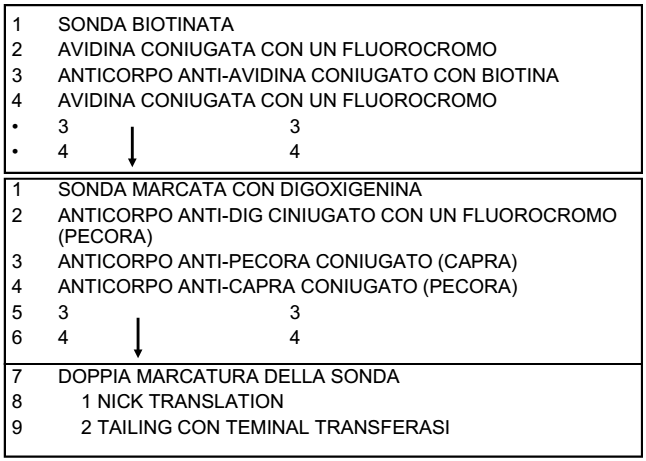
\includegraphics[width=0.46\textwidth]{img/36_amplificazione_segnale_fluorescente.png}
  \caption{Amplificazione del segnale}
\end{wrapfigure}

A questo punto ripeto gli step 3 e 4, perché evidenzio la Biotina con l’Avidina coniugata con il fluorocromo e poi utilizzo un anticorpo anti-Avidina biotinato, la Biotina la evidenzio con l’Avidina coniugata con il fluorocromo e così via aumentando gli strati.\\
In realtà più di 3/4 strati non si fanno, perché se aumento troppo gli strati aumento molto anche il background (in generale 3 strati sono già sufficienti per avere un’ottima amplificazione del segnale).

Seinvece si è utilizzata una sonda marcata con Digoxigenica quello che si farà sarà alternare gli animali in cui sono stati prodotti gli anticorpi, cioè uso anticorpi prodotti in un certo animale e poi anticorpi contro la parte costante dell’anticorpo di quel particolare animale.

\clearpage
Ad esempio:
\begin{itemize}
\item il primo strato è dato dalla sonda marcata con digoxigenina
\item poi uso un anticorpo primario prodotto in pecora anti-dig e coniugato con un fluorocromo
\item a questo punto uso un anticorpo \emph{anti-pecora}, ad esempio prodotto in capra, coniugato con un fluorocromo
\item poi uso un anticorpo \emph{anti-capra} prodotto in pecora coniugato con un fluorocromo, e così via.
\end{itemize}
Da questo momento in poi continuo alternando anti-capra e anti-pecora in più strati. Anche qui 3-4 strati sono sufficienti.\\
Importante è non avere cross-reattività fra gli anticorpi. Molto spesso può essere necessario colorare e vedere contemporaneamente su uno stesso preparato 4-5-10 sonde diverse che, per essere colorate in modo diverso, devono essere marcate in modo diverso e quindi poi possono essere evidenziate con una sequenza diversa di anticorpi specifici.

Attenzione: è importante che non ci sia cross-reattività fra gli anticorpi, quindi se uso una sequenza capra-pecora e un altro metodo di marcatura con un tracciante diverso e altri anticorpi, cercherò qualcosa di filogeneticamente molto lontano dalla capra e dalla pecora, per esempio uso anticorpi prodotti nei bovini oppure nell’asino, nel cavallo, nel pollo, nel topo (i più comuni sono gli anticorpi prodotti nel topo e in altri roditori). Più vado lontano filogeneticamente più sono sicuro che non ci sia cross-reattività fra gli anticorpi perché questo potrebbe essere molto pericoloso.

È anche possibile fare una doppia marcatura della sonda usando la nick-translatin e aggiungendo, con la \textbf{terminal-transferasi}, una coda marcata.

Per l’amplificazione del segnale si potrebbe anche usare la PCR, ma questa funziona male per via della dimensione dei frammenti: la lunghezza media dei frammenti per l'ibridaizone è di 700-1000 bp, mentre i frammenti amplificati dalla PCR sono molto più piccoli.
 
La lunghezza dei frammenti è importante perché io ottengo tanti frammenti tutti complementari alla sonda e quando li ibrido sul bersaglio, questi frammenti saranno localizzati a caso sulla sequenza bersaglio: se questi frammenti sono grossi si allineano e si sovrappongono parzialmente, cioè più grossi sono e più facilmente coprono tutto il segmento a cui sono complementari.

\subsubsection{Principio dell’albero di Natale per l’amplificazione del segnale}
In questo tipo di approcci, per l’amplificazione del segnale, si sfrutta lo stesso principio che si usa per l’immunofluorescenza, in particolare l’immunofluorescenza indiretta.\\
In generale per avere una maggiore intensità di marcatura fluorescente non si fa l’immunofluorescenza diretta ma indiretta, cioè si usa un primo anticorpo ``freddo'' (non marcato) e poi un anti-anticorpo ``caldo'' (marcato).

L’immunofluorescenza indiretta fa ricorso a quello che viene chiamato ``Principio dell’albero di Natale''. Partiamo dal target che voglio identificare, che è dotato di tanti epitopi: per prima cosa viene utilizzato un anticorpo freddo che si lega a ciascuno di questi epitopi, e ognuno di questi anticorpi primari legati funzionerà, a sua volta, da antigene per il secondo anticorpo (che è quello fluorescente), infatti ognuno di questi anticorpi primari, a sua volta, ha tanti epitopi, a ciascuno dei quali si legherà l’anticorpo secondario fluorescente.\\
Così, pur avendo usato soltanto due anticorpi, avrò un’enorme quantità di molecole fluorescenti che mi daranno segnale fluorescente.\\
Viene chiamato \emph{Principio dell’albero di Natale}, perché ad ogni strato anticorpo anti-anticorpo ho un’amplificazione a forma di abete al contrario. Questo amplifica enormemente il segnale fluorescente.

\subsection{I problemi della microscopia in fluorescenza}
Quando abbiamo a che fare con la microscopia in fluorescenza abbiamo due problemi fondamentali:
\begin{enumerate}
\item il \emph{``rumore''} della fluorescenza (background)
\item il \emph{decadimento} continuo della fluorescenza dovuto alla conversione, indotta dalla luce, del fluorocromo in un composto non fluorescente. Questo processo richiede luce e ossigeno.
\end{enumerate}

La \textbf{risoluzione} è la \emph{distanza minima che esiste fra due punti che possono essere ancora riconosciuti come separati}. Gran parte della risoluzione microscopica dipende dalla definizione dell’immagine microscopica. Con la fluorescenza tuttavia spesso vi è un ``alone di fluorescenza'' che fa sì che quando due spot fluorescenti sono molto vicini questi non possano essere distinti come separati ma risultino sovrapposti. Questo è un problema per la risoluzione microscopica, soprattutto quando si lavora con delle esigenze di risoluzione come nella FISH.\\ Questo è dovuto al rumore della fluorescenza, che fa diminuire la risoluzione.

Inoltre per evidenziare una molecola fluorescente questa deve essere esposta a una fonte luminosa che abbia la lunghezza d'onda adatta per eccitare il fluorocromo che sto utilizzando.\\
Eccitare la fluorescenza vuol dire che il fluoroforo emetterà ad una lunghezza d’onda che sarà dipendente dal fluoroforo che ho usato e dalla lunghezza d’onda incidente. L’emissione è dovuta al fatto che uno o più elettroni dell’orbitale più esterno decadono in un orbitale inferiore, quindi a un livello di energia inferiore, e questo decadimento produce un'energia che causa l’emissione alla lunghezza d’onda che mi permette di vedere l’emissione fluorescente. Quindi come io espongo alla luce UV il mio preparato perdo l’informazione, perché si ha decadimento della fluorescenza, quindi i preparati non sono permanenti ma soprattutto questo decadimento può essere molto rapido (addirittura può essere tanto rapido che io non riesco a registrare il dato).

Quindi c’è il decadimento continuo della fluorescenza dovuto alla conversione indotta dalla luce del fluoroforo in un composto non fluorescente e il processo avviene in presenza di luce e ossigeno.
Come posso eliminare la luce e l’ossigeno per ridurre questo fenomeno? Non posso eliminare la luce perché se non eccito il fluorocromo non posso avere emissione di fluorescenza, però posso eliminare l’ossigeno.\\
Vediamo quali sono le soluzioni che si adottano:
\begin{itemize}
\item \textbf{obiettivi ad alta apertura numerica} (N.A.)
\item uso di \textbf{fluorocromi fotostabili}
\item uso di \textbf{tamponi di montaggio antiossidanti} (per togliere l’ossigeno) che riducono di molto l’ossidazione quando i preparati vengono esposti alla luce
\item \textbf{riduzione al minimo della luce incidente}, perché più forte è la luce incidente (la luce ultravioletta in questo caso) e più veloce è il decadimento della fluorescenza. Per fare questo si usano \textbf{videocamere CCD (Charge Cloupled Device)}, cioè delle apparecchiature ad accoppiamento di carica. Queste sono videocamere a bassissimo livello di energia, cioè telecamere che riescono ad acquisire immagini con un livello di energia molto basso (in presenza di poca luce) ma con lunghe esposizioni. Queste telecamere vengono normalmente utilizzate in astronomia per catturare lunghezze d’onda provenienti da astri che non si vedono, con lunghissime esposizioni e sono state modificate per l’uso in microscopia a fluorescenza. Queste sono telecamere ad altissima sensibilità.\\
Associato all'utilizzo delle telecamere c'è poi un altro problema: in qualsiasi telecamera, a livello del fotosensore che acquisisce l’immagine, si genera un rumore che è associato all’emissione da parte del fotocatodo. Questo rumore di fondo (background) causa una diminuzione del rapporto tra rumore e immagine specifica causando una perdita di risoluzione. Questo rumore di fondo però può essere molto ridotto usando dei sensori raffreddati (esitono diversi sistemi di raffreddamento ma in generale c’è un circolo vizioso di una sostanza refrigerante).\\
Le telecamere CCD sono ad alta risoluzione, a basso livello di energia e raffreddate.
\end{itemize}

L’\textbf{apertura numerica} è una \emph{misura della capacità di una lente di convogliare e concentrare la luce sul preparato}. L’apertura numerica è \emph{inversamente proporzionale all’ingrandimento dell’obiettivo}: massima è l’apertura numerica e migliore è la risoluzione, proprio perché riesco a far convergere tutta la luce in un singolo punto che mi interessa, però l’aumento della risoluzione (cioè la capacità di ingrandimento dell’obiettivo) va a scapito dell’apertura numerica, quindi la risoluzione viene sensibilmente persa. D’altra parte per analizzare i cromosomi e soprattutto le fibre di DNA è necessario usare obiettivi che hanno il massimo ingrandimento: i cromosomi si guardano con obiettivi 100x che vuol dire 1000 ingrandimenti, se sommiamo quelli degli oculari.\\
La regola è quella di \emph{massimizzare il rapporto segnale/rumore} usando obiettivi con un ingrandimento minimo che permette una buona risoluzione: aumenta il rapporto segnale rumore a spese dell’ingrandimento.\\
Gli obiettivi che utilizziamo in questo tipo di lavori non sono da 100 ingrandimenti ma 63 e sono degli obiettivi dotati di quello che viene chiamato \emph{``diaframma di iride''} e cioè una ghiera che mi permette di variare l’apertura numerica a seconda del preparato che sto analizzando.
Con questi obiettivi si riesce ad ottimizzare la qualità delle immagini.\\
Il fatto di perdere un po’ in ingrandimento non è un grosso problema perché la risoluzione è talmente migliore, quindi la definizione dell’immagine è talmente migliore, che il risultato finale è comunque nettamente migliore rispetto a quello che si può ottenere utilizzando altri obiettivi 100x.

Le telecamere migliori non lavorano a colori ma in bianco e nero, ovvero acquisiscono l’immagine sulla base del rapporto di intensità di toni di grigio. Questo permette di avere uno spettro enorme di acquisizioni con variazioni di intensità di toni di grigio anche molto piccole (ogni tono di grigio corrisponde a una particolare lunghezza d'onda di un fluorocromo), aumentando enormemente la risoluzione.

Oggi le telecamere costano meno, ma in compenso i software necessari per analizzare le immagini costano molto di più.\\
Questi software permettono:
\begin{itemize}
\item di \textbf{collezionare e memorizzare le immagini}
\item di \textbf{assegnare pseudocolori} sulla base di una scala di toni di grigio. Le immagini devono essere pseudocolorate così da riflettere il colore del fluorocromo utilizzato per marcare una particolare sonda o una sequenza o una particolare regione della cellula.
\item di \textbf{fare il merging delle singole immagini}. 
Questo viene fatto sovrapponendo tutte le diverse immagini che si sono acquisite per ogni tipo di fluorocromo utilizzato.\\
I microscopi costano molto anche perchè esistono dei sistemi automatizzati che permettono di cambiare il filtro utilizzato avendo la certezza di non muovere il vetrino e dunque avendo la certezza che le immagini rimangano assolutamente allineate tra loro.\\
È assolutamente fondamentale che le immagini rimangano perfettamente allineate perché i risultati che otteniamo sono \emph{quantitativi} e se voglio misurare la distanza tra due sonde (due geni, due sequenze) devo essere sicura che l’allineamento sia perfetto perché basta pochissimo per cambiare completamente il risultato.
\item di \textbf{ridurre il rapporto segnale-rumore}.
Questi software permettono di modificare i parametri di esposizione per ridurre il più possibile il rapporto segnale-rumore anche mentre si acquisisce l’immagine.\\
Questo è fondamentale perché devo acquisire un dato che sia scientificamente significativo ma che può non essere apprezzabile se l’esposizione è sbagliata e quindi il rapporto segnale-rumore non è il rapporto ottimale.
Se non si ha questo software che riduce direttamente il rapporto segnale-rumore, le immagini dovranno essere elaborate su altri computer con Photoshop. Ma, per quanto il tipo di elaborazione che si fa è semplicemente un enfatizzare il segnale specifico e ridurre quello che è aspecifico (modificando i rapporti di intensità di fluorescenza in generale), per documentare su un paper scientifico l’immagine, quando si fa un’elaborazione con Photoshop, si deve dichiarare esattamente quello che si fa, non si può inventare un dato: devo dare un dato che sia molto eloquente e un’immagine che sia esplicita in maniera immediata. È evidente che l’elaborazione con Photoshop può lasciare delle perplessità: devo quindi spiegare esattamente che tipo di elaborazione è stata fatta e non si possono ingannare i reviewer perché è possibile ricostruire esattamente tutto quello che è stato fatto con Photoshop su qualunque immagine, resta traccia di qualunque elaborazione sia stata fatta.  
Quindi è molto importante che queste nuove CCD camere siano associate a software che permettono di farlo direttamente: quando acquisisco l’immagine, l’acquisisco già al suo meglio e non ho bisogno poi di migliorarla per renderla scientificamente esplicita a posteriori con Photosop.
\item di \textbf{misurare dimensione e distanza tra i segnali}.
Grazie a questi software è possibile fare anche delle misurazioni delle distanze tra i segnali, dell’intensità dei segnali e di diversi altri parametri per avre dati che siano anche quantitativi e non solo qualitativi. La citogenetica molecolare ad alta risoluzione è un metodo quantitativo, non semplicemente un approccio qualitativo come il metodo morfologico classico.
\end{itemize}


\section{La microscopia confocale}
La microscopia a fluorescenza non è l'unico tipo di microscopia che permette di fare analisi ad alta risoluzione, ma esiste anche la microscopia confocale. 

L'ultima generazione di microscopi confocali è rappresentata dai microscopi STED, i quali però hanno costi altissimi (600mila euro contro i 160mila di un microscopio a fluorescenza).

La microscopia elettronica si trova all'interfaccia tra la microscopia ottica e quella elettronica: l'impianto del microscopio è analogo a quello dei microscopi ottici a fluorescenza, tuttavia il microscopio confocale è collegato a uno o più fasci laser, è dunque un \textbf{microscopio a scansione laser}.

In questo caso l’acquisizione delle immagini avviene attraverso la scansione: il preparato in questo caso viene scansionato non solo in maniera orizzontale, di superficie, ma anche verticalemnte, permettendo di ottenere foto di sezioni a diversa profondità del campione. Questo è molto importante perché un preparato di microscopia ottica ha uno spessore e normalmente, quando si mette a fuoco, si acquisisce l’immagine con il fuoco migliore per quello che si vuole vedere, ma lasciando molte cose fuori fuoco. Questi dettagli fuori fuoco andranno poi a creare una sorta di rumore attorno a ciò che si vuole osservare e causeranno una perdita della definizione e della risoluzione delle immagini.

Questi microscopi permettono dunque di aumentare la risoluzione perché le sezioni trasversali (fettine) del preparato vengono analizzate indipendentemente mentre tutti i segnali generati da piani focali diversi vengono eliminati.
  
La sorgente di eccitazione della fluorescenza è un fascio laser: i più usati sono quelli ad \emph{Argon} o a \emph{Cripton} e quindi le lunghezze d’onda sono \emph{330 o 600 nm}. Questo rappresenta un primo limite in quanto non esistono microscopi confocali con più di due fasci laser e questo riduce il numero di molecole fluorescenti che si possono utilizzare. 

L’immagine ottenuta con il microscopio confocale è \emph{tridimensionale} perché c’è un software dedicato che fa la sommatoria, l’integrale, delle singole immagini sui singoli piani focali.

Lo svantaggio di questo microscopio rispetto alla microscopia in fluorescenza con telecamere ad alta risoluzione è il numero di fluorocromi che posso utilizzare, mentre i vantaggi sono l’aumento della risoluzione e la possibilità di avere immagini tridimensionali.\\
A seconda delle esigenze si sceglierà lo strumento più adatto.

\section{L'ibridazione in situ con competizione}
Quando facciamo delle ibridazioni in situ, approccio che serve soprattutto per l’analisi dei genomi complessi (e.g. genomi di eucarioti superiori e soprattutto dei mammiferi) normalmente disponiamo di sonde clonate in BAC (cromosomi artificiali batterici). 
Una \textbf{sonda clonata in BAC} rappresenta un segmento di genoma dell’ordine di grandezza di \emph{150-200 Kb} che, essendo un segmento di genoma di grosse dimensioni, non contiene soltanto singoli geni.

Più o meno l’1\% del genoma è costituito da geni che codificano per proteine, poi ci sono sequenze di RNA non codificante e poi circa il 50\% (47-46\%) del genoma di tutti i vertebrati superiori e in particolare dei mammiferi è costituito da DNA ripetuto. La gran parte di questo DNA ripetuto è costituito da sequenze molto simili tra loro e distribuite a pioggia in tutto il genoma (\emph{DNA ripetuto intersperso}.

Sapendo questo risulta abbastanza evidentemente che se si usa un segmento genomico di 150mila paia di basi al suo interno si avrà una sequenza a singola copia ma certamente anche un gran numero di sequenze altamente ripetute. Quindi, se si usa tal quale una sonda di questo tipo, la cinetica di ibridazione sarà molto maggiore per le sequenza ripetute rispetto alle sequenze a singola copia che vogliamo evidenziare semplicemente perché di sequenze a singola copia ce n’è una mentre le sequenze ripetute sono moltissime e quindi, in una sospensione, la probabilità che le sequenze ripetute si trovino tra loro e che formino eteroduplex è molto più alta rispetto alla probabilità che si trovino le sequenze uniche.\\
Per questa ragione se si usa semplicemente una sonda che rappresenta un segmento genomico si otterrà come risultato che questa si ibridi in maniera uniforme in tutto il genoma. Ecco allora che è fondamentale applicare la tecnica dell'\textbf{ibridazione in situ con competizione (Chromosomal In Situ Suppression - CISS)} o \textbf{ISSH (In Situ Suppression Hybridisation)}.

\begin{wrapfigure}{r}{0.6\textwidth}
    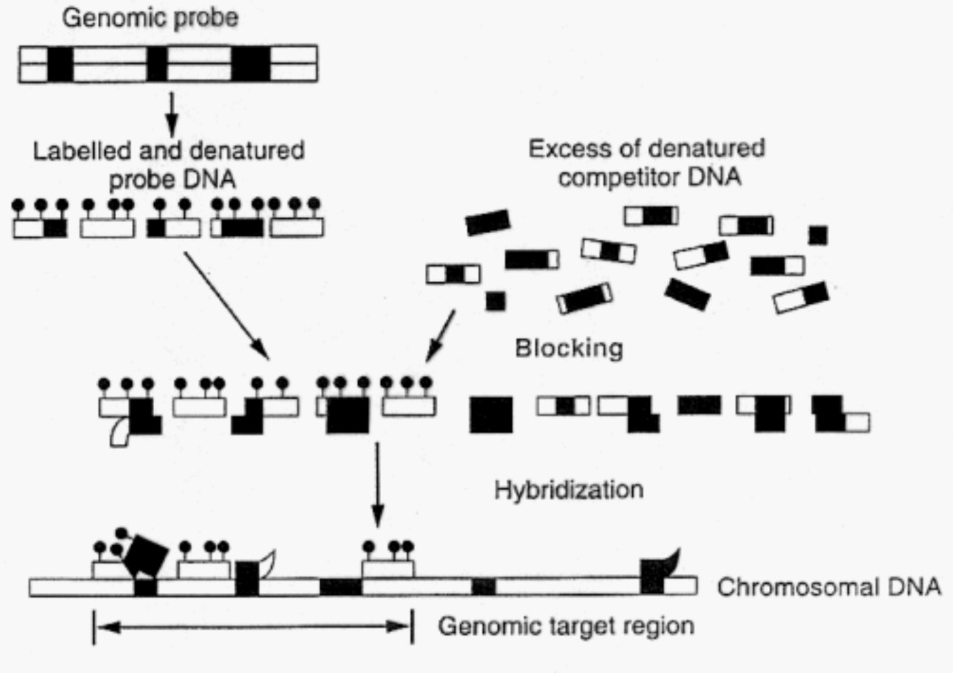
\includegraphics[width=0.6\textwidth]{img/38_competizione.png}
  \caption{Ibridazione con competizione}
\end{wrapfigure}

La sonda inizialmente non è altro che un segmento genomico clonato in BAC, contenente sia la sequenza singola che le sequenze ripetute, che verrà marcata per nick translation e denaturata. A questo punto, prima di ibridarla, la sonda verrà miscelata con del DNA genomico\textbf{*} della stessa specie: grazie all'elevata cinetica di rinaturazione-ibridazione delle sequenze altamente ripetute basterà un quarto d'ora perchè queste si leghino.
Nell'immagine le parti scure rappresentano le sequenze ripetute intersperse, quelle che devo sottrarre.

\textbf{*}Si può anche usare del DNA arricchito di sequenze ripetute, ma va benissimo anche il DNA genomico perché ha comunque un’enorme quantità di sequenze ripetute intersperse uguali a quelle presenti nel mio segmento e una minoranza di sequenze a singola copia: non serve che io spenda per comprare il DNA arricchito in sequenze ripetute, faccio un’estrazione del DNA genomico della stessa specie, lo frammento e poi prendo il DNA competitore, anche questo denaturato, e prima di ibridare la sonda, la metto in presenza di questo DNA competitore.

Una volta trascorso il tempo necessario la sonda presenterà dei ``tappi molecolari'', ovvero i frammenti di DNA competitore che erano stati inseriti nella miscela si saranno legati alle sequenze complementari ripetute della sonda. A questo punto la sonda presenterà solo alcune zone ancora a singola elica e disponibili all'ibridazione e quelle zone saranno proprio quelle a singola copia che conferiranno specificità al segnale fluorescente.

Questa tecnica è fondamentale soprattutto quando si parla di quelle metodiche che permettono di avere delle immagini di cariotipi a mille colori in cui tutti i cromosomi o addirittura tutti i bracci di ogni cromosoma sono di un colore diverso, perché si potrà usare come sonda il DNA di interi cromosomi fisicamente isolati: queste si chiamano painting probes. 

\section{Le painting probes}
Esistono diverse tecniche che permettono di isolare fisicamente un singolo cromosoma.\\
Tra queste tecniche c'è l'utilizzo delle sonde che abbiamo appena descritto che mi permetteranno di riconoscere sequenze specifiche di un cromosoma senza tener conto delle sequenze ripetute condivise da tutti i cromosomi. Questo viene definito \textbf{``chromosome painting''}\\
Questo è molto importante soprattutto se, ad esempio, supponiamo di avere come campione il DNA di una cellula tumorale. Normalmente, nei tumori solidi, il cariotipo presenta riarrangiamenti molto complessi in cui addirittura ci sono cromosomi marcatori con 10 punti di rottura. In questo caso si parla di \textbf{``cromosomi arlecchino''}, dove i diversi segmenti derivano tutti da cromosomi diversi tra loro.\\
Capire da quali tasselli siano composti questi cromosomi arlecchino tramite approcci di bandeggio convenzionale non è possibile, mentre lo è se si utilizzano delle painting probes capaci di riconosce i vari tasselli e di colorarli tutti di colori diversi.\\
Questo è un approccio fondamentale per identificare dei marcatori con riarrangiamenti complessi.

È anche possibile fare il \textbf{``reverse chromosome painting''}, in cui si ha un marcatore cromosomico di cui non si conosce l'origine, ovvero non si sa da quale cromosoma derivi, perché è riarrangiato o perchè è un micro-cromosoma. In questo caso si può isolare, marcare e far ibridare questo pezzo di cromosoma su una mitosi normale e osservare su quali cromosomi si andrà ad ibridare, capendo così da che cromosomi deriva.

Questi approcci sono potentissimi soprattutto nelle loro applicazioni cliniche.

\section{La FISH a due o più colori}

\begin{wrapfigure}{r}{0.42\textwidth}
    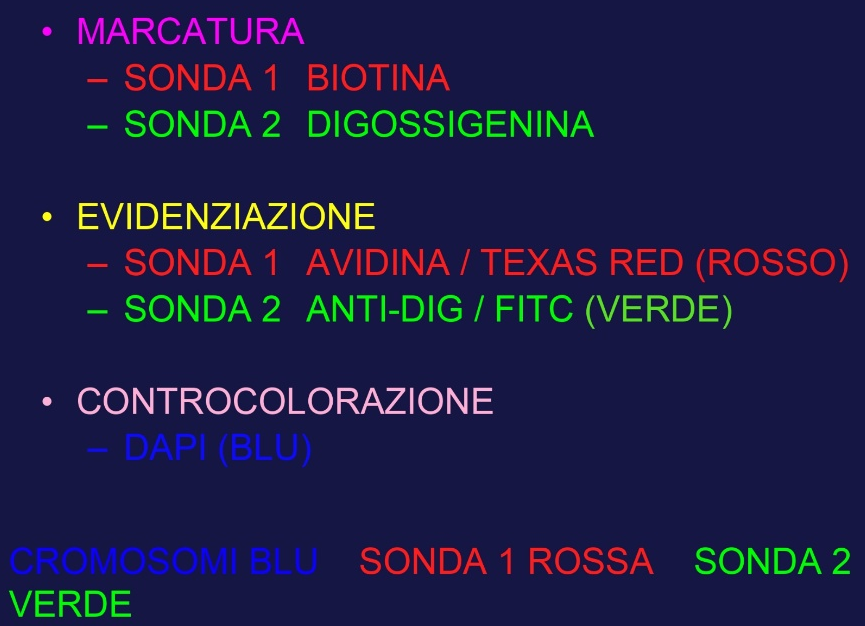
\includegraphics[width=0.4\textwidth]{img/39_fish_due_colori.png}
  \caption{FISH a due colori}
\end{wrapfigure}


La FISH può anche essere condotta con più sonde punchè queste siano marcate diversamente ed è utile quando si vuole capire quanto sono distandi due sequenze, se sono sovrapposte o se sono presenti certi riarrangiamenti.\\
In questi casi avrò bisogno di un microscopio con 3 filtri: 2 filtri per i due diversi fluorocromi utilizzati per marcare le due sonde e un filtro per osservare i cromosomi che saranno sempre controcolorati con il DAPI (la colorazione con il DAPI è sovrapponibile ad un bandeggio Q).
Ognuno di questi sarà poi pseudocolorato con colori diversi.

Le due sonde, ovviamente, dovranno essere marcate in maniera diversa, ad esempio la sonda 1 sarà marcata con la biotino e la 2 con la digossigenina, ognuna di loro poi sarà riconosciuta da un anticorpo e dall'avidina a loro volta marcati con un diverso fluorocromo.

Nella \textbf{FISH a più colori} invece si passa da 2 colori a 7 colori: anche qui i cromosomi sono sempre controcolorati in blu con il DAPI, ma uso 3 sistemi di marcatura (non più due) che saranno: biotina, digossigenina e infine una marcatura diretta con la fluoresceina (si usa UTP già coniugato con il fluorocromo).\\
La FISH a più colori, se non si supera un certo numero di colori, può essere fatta in maniera ``casalinga'' senza avere dei sistemi di marcatura commerciali e senza necessità di un software dedicato.\\
La FISH a più colori si può fare con un qualunque microscopio a fluorescenza.

Seguendo quanto appena detto però si piò arrivare solo ad una marcatura a 3 colori (+ il DAPI). Come si fanno dunque ad osservare 7 sonde diverse se si possiedono solo 4 filtri diversi?\\
Semplicemente si marcano le sonde con gli stessi marcatori ma in concentrazioni diverse. Ad esempio, supponendo di marcare:
\begin{itemize}
\item la sonda 1 con biotina che verrà riconosciuta dall'avidina coniugata con Ultralite (emette nell'ultravioletto)
\item la sonda 2 con digossigenina coniugata con rodamina che emette nel rosso
\item la sonda 3 con fluoresceina che emette nel verde.
\end{itemize}

\begin{wrapfigure}{r}{0.42\textwidth}
    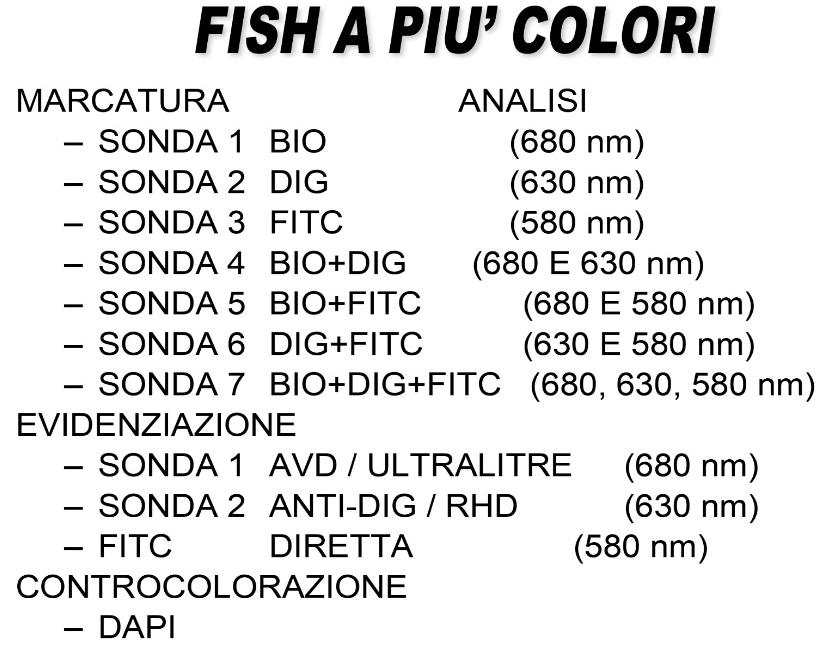
\includegraphics[width=0.4\textwidth]{img/40_fish_multicolore.png}
  \caption{FISH multicolore}
\end{wrapfigure}

Per ognuna di queste sonde avrò bisogno di un filtro apposito, oltre al filtro per il blu (DAPI).\\
Tuttavia, se si marcano le sonde con miscele diverse di marcatori sarà possibile vedere tutte queste sonde semplicemente utilizzando combinazioni diverse di filtri.

Ad esempio:
\begin{itemize}
\item la sonda 1 è l'unica che si vede esclusivamente con il filtro a 680 nm
\item la sonda 2 è l’unica che vedo solo con il filtro a 630 nm
\item la sonda 3 è l’unica che vedo con il filtro a 580 nm
\item la sonda 4 la marco con una miscela 1:1 di biotina e digossigenica, quindi la potrò vedere con l’accoppiamento di filtri 680-630 nm
\item la sonda 5 (biotina e fluoresceina) è l’unica che vedo con il 680, ma non con il 630, bensì con il 580
\item la sonda 6 (dove ho messo digossigenina e fluoresceina) è l’unica che vedo con il 630 e con il 580
\item l’ultima sonda la marco con una miscela 1:1:1 di UTP coniugato con ciascuno dei sistemi di marcatura e quindi è l’unica che vedo con tutti e tre i filtri.
\end{itemize}

A questo punto sarà necessario pseudocolorare ogne immagine con uno pseudocolore a seconda dei filtri utilizzati, per esempio: pseudocolore del colore 1 tutte le immagini che vedo \emph{solo} con il primo filtro, del colore 2 quelle che vedo \emph{solo} con il secondo, del colore 3 quelle che vedo \emph{solo} il terzo filtro, del colore 4 quelle che vedo soltanto con una coppia di filtri, del colore 5 per un’altra coppia di filtri, colore 6 per l’ultima coppia di filtri e infine colore 7 per il terzetto di filtri.

Come avviene l’osservazione con più filtri?
Semplicemente si guarda il preparato più volte con filtri diversi e per ogni filtro si registrano i vari segnali, dopodichè si sovrappongono le immagini e si vede in quali punti vi sono più di uno pseudocolore capendo così quale sonda vi si è legata. Anche qui sarà fondamentale avere dei sistemi che permettano di cambiare filtro senza muovere il preparato.

Ogni immagine osservata con un singolo filtro viene acquisita in scala di grigi, solo alla fine avrò le singole immagini a cui avrò assegnato un diverso pseudocolore che potrò ottimizzare e poi sovrapporre tramire un software apposito.

L'utilizzo di queste 7 sonde su un singolo cromosoma mi permette di sapere in che sequenza sono, a che distanza si trovano e di avere moltissime altre informazioni in proposito.

È fondamentale capire il principio alla base di questa tecnica perché il poter passare da 7 a 24 e più colori non è altro che un’estensione dello stesso identico principio. I metodi di marcatura di solito non sono più di 4, ma le miscele sono in rapporti diversi: per esempio, anziché 1:1 si può usare una miscela con rapporto 1:3. Cambiando il rapporto tra i marcatori cambierà il rapporto di toni di grigio e questo verrà registrato dal software che mi permetterà di distinguerli e di apprezzare la varie differenze.

Quindi anche con pochi sistemi di marcatura, se si fanno miscele diverse con rapporti diversi (anziché 50 e 50 posso fare 1:3 o 1:4 ecc), si possono aumentare enormemente il numero di colori senza avere mille sistemi di marcatura. C’è un limite ai sistemi di marcatura che posso utilizzare come c’è un limite per i fluorocromi, ma non c’è un limite al numero di pseudocolori perché me li invento. Gli pseudocolori dipendono dal rapporto di intensità di grigio tra un fluorocromo e l’altro.
Per questi scopi non si può usare il confocale perché con il confocale posso usare al massimo 2 fasci laser e quindi due metodi di marcatura.

\subsubsection{Riassumendo}
\begin{itemize}
\item Le immagini ottenute alle diverse lunghezze d’onda vengono acquisite indipendentemente in bianco e nero e archiviate
\item Le singole immagini vengono elaborate per ottimizzare i parametri di acquisizione per ogni lunghezza d’onda.
\item Poi viene attribuito un diverso pseudocolore ad ogni sonda.
\item Un software dedicato consente poi di fare il merge e cioè di sovrapporre le singole immagini pseudocolorate e ottenere un’immagine dove i cromosomi sono blu e poi ci sono sopra colori diversi.
\end{itemize}


\section{La M-FISH o SKY FISH}
Il principio appena esposto viene usato anche per fare quelle che vengono chiamate \textbf{M-FISH (Multicolor FISH)} o \textbf{Sky FISH} che permettono di fare i cosiddetti \textbf{``spectral karyotype''}. Siccome sono quelle che permettono di colorare tutti i cromosomi di colori diversi, si usano delle painting probes.\\
Quindi il pool di DNA di ogni cromosoma umano viene direttamente marcato con UTP coniugato ad 1, 2 , 3, 4 o 5 fluorocromi, dipende. Per fare questo ci sono delle company che vendono dei kit: queste miscele calibrate non si possono fare in casa e quindi costa molto fare questi esperimenti. I rapporti di concentrazione dell’UTP coniugato con i diversi fluorocromi nella miscela di nick translation è tale da generare una marcatura di colore diverso, ma intesa come rapporto di intensità di grigio diverso per ogni cromosoma. Poi pseudo coloro in modo diverso.\\
Anche qui la misurazione della variazione di rapporti di toni di grigio e la pseudocolorazione sono fatte da un software dedicato, non riesco a farle in maniera artigianale. Poi pseudocoloro ogni cromosoma a seconda dei rapporti di intensità di toni di grigio dei diversi sistemi di marcatura.\\
L’occhio umano naturalmente non riesce a distinguere i 24 colori creati dal rapporto di fluorocromi nelle miscele di reazione. Con 5 filtri, uno specifico per l’eccitazione di ciascuno dei metodi di marcatura utilizzati, le immagini vengono acquisite come scala di grigio e memorizzate. Quindi poi pseudocoloro con un diverso pseudocolore per ogni intensità di grigio ossia per ogni cromosoma. Le singole immagini pseudocolorate vengono sovrapposte (merged): si ottiene un’immagine della metafase con ogni cromosoma di un colore diverso e quindi un cariotipo a 24 colori. Addirittura si arriva a colorare ciascun braccio cromosomico di un colore diverso.\\
Mi devo procurare dei kit di marcatura per i singoli cromosomi e un software che mi permetta di fare l’analisi e la pseudocolorazione dei diversi rapporti di toni di grigio tra 5 fluorocromi utilizzati contemporaneamente.

\begin{wrapfigure}{r}{0.6\textwidth}
    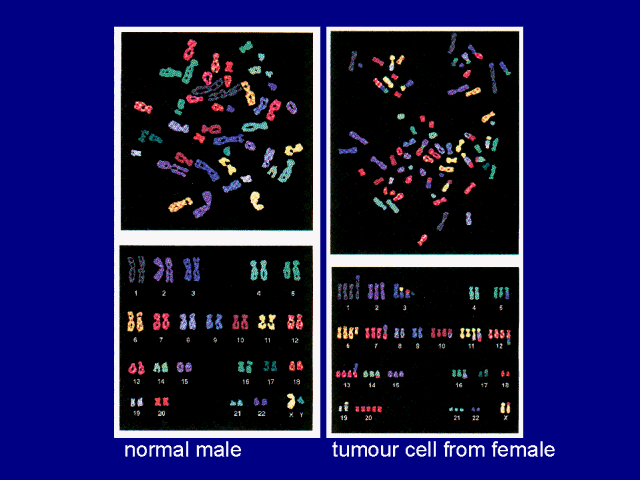
\includegraphics[width=0.6\textwidth]{img/41_cariotipo_fish.png}
  \caption{Cariotipo normale e tumorale in SKY FISH}
\end{wrapfigure}

Questo approccio viene usato normalmente per l’analisi dei cariotipi molto riarrangiati nelle cellule tumorali, oltre che per l’identificazione di marcatori cromosomici.\\
Ad uno stadio avanzato della progressione del tumore ci sono moltissimi riarrangiamenti e inoltre i cariotipi dei tumori solidi in stadio avanzato sono veramente un puzzle di segmenti cromosomici e, guardando l’immagine sotto, è palese che varia il numero cromosomico. 

Un’analisi di questo tipo ha cambiato il volto della citogenetica oncologica. Prima non esisteva la citogenetica oncologica dei tumori solidi proprio perché era impossibile riuscire a districarsi tra riarrangiamenti così complessi.\\
I tumori solidi sono differenti rispetto alle leucemie. Nelle leucemie faccio l’analisi del midollo quindi riesco ad analizzare le cellule primordiali tumorali e quindi riesco ad analizzare i primi riarrangiamenti. I tumori solidi invece si analizzano a partire da un prelievo bioptico del tumore, quando già è in uno stadio abbastanza avanzato e quindi quando già ci sono tanti riarrangiamenti.\\
L’analisi citogenetica dei tumori consente di capire, identificando i punti di rottura, quali sono i geni coinvolti nello sviluppo, nell’eziologia, ovvero quelli causativi del cancro, ma consente anche di capire quali sono i geni coinvolti nel processi di progressione e metastatizzazione. Quindi l’approccio citogenetico è fondamentale per la comprensione dei meccanismi di sviluppo e di evoluzione dei tumori.

È evidente che, se in un tumore ho dei riarrangiamenti coì complessi, capire qual è quello causativo e qual è quello secondario non è banale, ma dal momento che oggi abbiamo delle banche dati che raccolgono le informazioni da tutti i laboratori del mondo e riportano tutti i riarrangiamenti coinvolti nello stesso tipo di tumori, ci si può avvicinare all’identificazione (e in qualche caso è stato fatto) del riarrangiamento che rappresenta il minimo comune denominatore di tutti i tumori della stessa classe. Per fare questo ovviamente bisogna avere un gran numero di dati.


\section{Comparative Genomic Hybridization - CGH}
La CGH è una tecnica straordinaria perché permette di fare delle analisi citogenetiche (cioè identificare riarrangiamenti cromosomici) senza bisogno di avere il cariotipo delle cellule in cui si vuole scoprire il riarrangiamento. 

Normalmente per fare analisi di citogenetica è necessario avere delle cellule che siano in attiva replicazione così da poter marcare i cromosomi, ma uno dei problemi della citogenetica dei tumori solidi è che normalmente si hanno dei campioni il cui materiale non è adatto per fare le analisi: il materiale risulta adatto se riesco a fare delle linee cellulari, ma nel momento in cui io impianto una linea cellulare questa si è già adattata alle condizioni in vitro e quindi resterà un punto interrogativo su quanto questa sia simile al tumore di partenza.

Con la CGH invece è possibile fare l’analisi cromosomica dei riarrangiamenti presenti nel cancro anche avendo un prelievo necrotico o cellule che non si replicano, perchè sfrutta semplicemente il DNA. Il DNA infatti è una molecola molto resistente che può essere estratta e isolata anche da cellule necrotiche.

Il limite è che la CGH, al contrario della Sky FISH, non va bene per i riarrangiamenti bilanciati (traslocazioni o inversioni, scambi), ma va bene per i \textbf{riarrangiamenti sbilanciati} e cioè tutti i riarrangiamenti che comportano la perdita o l’acquisto di regioni genomiche (delezioni e duplicazioni) anche in assenza di divisione cellulare.

La Sky FISH permette di vedere soprattutto traslocazioni, non delezioni o duplicazioni: le traslocazioni sono tasselli di colore diverso, ma nelle delezioni e nelle duplicazioni o manca un pezzetto o un pezzetto è raddoppiato e quindi è difficilmente apprezzabile perché non c’è lo scambio di colori.

La CGH è particolarmente utile per l’analisi di materiale qualitativamente scarso o per campioni di tessuto molto poveri o per cellule che non si replicano.\\
È ideale per l’analisi di riarrangiamenti complessi, purchè prevedano alterazioni del dosaggio.

\emph{Come funziona?}\\
Il DNA genomico viene estratto da cellule che si suppone abbiano riarrangiamenti, come  nel nostro esempio la biopsia del cancro. Le cellule vengono omogenizzate, si estrae il DNA e lo si purifica, si fa l’estrazione di tutte le proteine. Alla fine si ottiene in una provetta il campione del DNA genomico della cellula da testare che chiamiamo \textbf{DNA test} (DNA genomico della cellula tumorale purificato).\\
Il \emph{DNA test} viene marcato con \emph{biotina}, poi si prende del DNA genomico da cellule di controllo di un individuo sano e lo marco in maniera diversa, ad esempio con digossigenina.\\
A questo punto si fa una miscela 50-50 del DNA test e del DNA di controllo marcati in modo diverso e li si ibrida su cromosomi normali di un controllo.\\
L’ibridazione dunque viene fatta su cromosomi che so essere perfettamente normali: la miscela 1 a 1 delle due sonde si ibrida con i cromosomi normali e poi evidenzio le due differenti sonde, una in verde e una in rosso.\\
Cosa mi aspetto di vedere? Innanzitutto vedrò tutti i cromosomi dello stesso colore giallo (sovrapposizione delle due diverse sonde), ma nel caso in cui ci sia una duplicazione in una certa regione, allora per quella regione, non ci sarà un rapporto 1 a 1 tra quello che è marcato di verde e quello che è marcato di rosso, ma ci sarà un eccesso di una delle due sonde (quella con cui abbiamo colorato il DNA tumorale). In quella regione dove nel cancro c’era una duplicazione, sui miei cromosomi non avrò giallo, ma avrò un eccesso di rosso e quindi lo vedrò come una bandina di colore diverso.\\
Se viceversa c’era una delezione avrò un eccesso di verde (colore con cui ho marcato il DNA di controllo) e un difetto di rosso e quindi lo vedrò come un rapporto di fluorescenza diverso rispetto all’atteso.\\
In alcuni casi questo è eclatante e lo si vede ad occhio nudo.

Normalmente ci si aspetterebbe un rapporto di fluorescenza verde/rosso pari a 1 e si ha un software che scansiona e calcola il rapporto di fluorescenza punto per punto su tutti i cromosomi mettendo in evidenza i punti del cromosoma in cui il rapporto è diverdso da 1 come dei picchi su un grafico.

Per questa tecnica è dunque fondamentale che il bersaglio siano cromosomi normali, perchè è solo su questi chesi riesce a vedere se c’è duplicazione o delezione.

In questo periodo in cui è protagonista la genomica e la post-genomica, protagonista è anche la citogenomica che è una citogenetica fatta con approcci di post-genomica.\\
Questa tecnica, così com’è, viene fatta utilizzando dei microchip. Tenendo presente lo stesso principio di prima, anziché avere come bersaglio della miscela 1 a 1 delle sonde il cromosoma si avrà come bersaglio un microchip.
Il microchip è un vetrino su cui sono spottate delle microquantità di particolari regioni genomiche. Posso farlo whole-genome, ma posso anche analizzare un particolare segmento cromosomico.\\
Questi microchip sono prodotti da delle company a cui posso richiedere di creare un microchip con un certo tratto di genoma specifico derivante da BAC (migliore risoluzione rispetto al cromosoma). 
Su questi vetrini si farà poi l'ibridazione con la miscela 1:1 DNA test-DNA controllo e infine vi sarà un sistema di analisi automatizzato che farà la scansione del vetrino e segnalerà gli spot con eccesso di rosso o di verde.

Questa tecnica è fondamentale perché consente di identificare non tanto i riarrangiamenti dei tumori, ma soprattutto le \textbf{copy number variation}, che sono fondamentali in molte patologie.


\chapter{L'isolamento dei cromosomi}
L’ibridazione in situ è strettamente correlata con l’isolamento dei cromosomi poiché per ottenere le painting probes è necessario disporre di sonde che coprano singoli cromosomi e quindi è necessario poter isolare i singoli cromosomi, estrarre il DNA, clonarlo, amplificarlo e poi marcarlo.

Gli approcci utilizzati per l’isolamento dei cromosomi sono:
\begin{enumerate}
\item Ibridazione di cellule somatiche
\item Citofluorimetria a flusso - ``Chromosome sorting''
\item Microdissezione
\end{enumerate}


\section{L'ibridazione di cellule somatiche}
L’ibridazione di cellule somatiche è a tutti gli effetti un metodo per disporre di cromosomi isolati.
Ricordiamo che è possibile ottenere ibridi mono-cromosomici per tutti i cromosomi inserendo dei marcatori che permettano di fare una selezione direzionale per il mantenimento di quel particolare cromosoma.\\
In realtà, una volta estratto il DNA dall’ibrido mono-cromosomico, nella provetta si ottiene un eccesso di genoma del roditore ed un singolo cromosoma umano.

Nonostante ciò, fare ibridi somatici mono-cromosomici è equivalente ad avere quel singolo cromosoma umano come se fosse purificato e isolato in una singola provetta.\\
Questo perché le sequenze altamente ripetute intersperse a pioggia in tutto il genoma sono specie-specifiche.\\
Fondamentalmente si tratta delle sequenze \textbf{LINE (Long Interspersed Nuclear Element)} e delle sequenze \textbf{SINE (Short Interspersed Nuclear Element)} che, in realtà, sono intersperse nel genoma in maniera non del tutto casuale:
\begin{itemize}
\item le SINE sono più concentrate nelle regioni intergeniche, cioè nelle regioni in cui si trovano i geni
\item LINE sono più concentrate nelle regioni intrageniche
\end{itemize}

Le più famose sequenze altamente ripetute intersperse specifiche del genoma umano sono le \textbf{Alu}, che sono delle \emph{SINE}.\\
Questi elementi, che tra l’altro sono tutti elementi retro-trasponibili più o meno completi, hanno un’altissima specie-specificità e, dal momento che la sequenza di specifiche famiglie di LINE e di SINE è altamente conservata, è possibile costruire dei primer sulla base della sequenza di queste sequenze ripetute e intersperse.

Fondamentalmente, se si effettua una \textbf{Alu-PCR}, cioè se si fa un’amplificazione del DNA globale dell’ibrido somatico utilizzando come primer delle sequenze ALU, si amplifica esclusivamente il DNA umano presente nella miscela di frammenti che si stanno amplificando.
Quindi, attraverso una semplice PCR è possibile ottenere un enorme arricchimento esclusivamente del DNA umano presente nell’ibrido.
 
La creazione di ibridi mono-cromosomici è quindi assolutamente da considerare come una tecnica di isolamento dei cromosomi in quanto avere un cromosoma isolato in un ibrido monocromosomico o un segmento cromosomico isolato in un ibrido da radiazione è sperimentalmente identico ad avere quel singolo cromosoma o segmento cromosomico purificato in una provetta.

\section{La citofluorimetria a flusso – Chromosome sorting}
In questo caso parliamo di qualcosa di più della semplice citofluorimetria perché parliamo di \textbf{citofluorimetri a flusso separatori (FACS - Fluorescence Activated Cell Sorter)}.

Un citofluorimetro è uno strumento che consente di misurare l’intensità di fluorescenza di particelle spontaneamente fluorescenti o che sono state colorate con un particolare fluorocromo e di ottenere un profilo che darà:
\begin{itemize}
\item sull’asse delle ascisse l’intensità di fluorescenza emessa 
\item sull’asse delle ordinate il numero di particelle con quella fluorescenza
\end{itemize}

Mettiamo il caso di avere un espianto bioptico e di voler sapere quanto siano rappresentate le cellule tumorali e teniamo in considerazione che le cellule tumorali sono generalmente eteroploidi, cioè non hanno un cariotipo diploide ma, in generale, hanno un cariotipo iperdiploide.
In particolare, le cellule tumorali hanno anomalie numeriche che portano il numero dei cromosomi ad essere superiore a quello normale diploide. 
Normalmente, quando il tumore è in fase molto avanzata il numero cromosomico è pari a 50-60 cromosomi, quindi le cellule tumorali hanno un contenuto di DNA nettamente diverso rispetto alla popolazione di cellule normali.

Allora, se si vuole vedere quanto è rappresentata la popolazione di cellule tumorali nel campione rispetto alle cellule normali (perché naturalmente qualsiasi biopsia sarà contaminata da cellule normali, non saranno presenti solo cellule tumorali. Questo da un punto di vista diagnostico ci dà un’idea di quanto aggressivo e invasivo sia il tumore) si può fare con la citofluorimetria, che consente di vedere il contenuto di DNA delle cellule e vedere così se ci sono due sottopopolazioni, una con un contenuto diploide e l’altra con un contenuto superiore a quello diploide.

Quindi, il citofluorimetro misura fondamentalmente la fluorescenza.\\ Naturalmente se il fluorocromo, come nell’esempio, è un colorante affine al DNA, come il bromuro di etidio (un intercalante), sarà possibile valutare la quantità di DNA nelle cellule.


\subsection{Citofluorimetri a flusso separatori}

I citofluorimetri a flusso separatori non si limitano alla parte analitica ma possono separare tutto ciò che ha un’intensità di fluorescenza emessa sufficientemente diversa dal resto della popolazione.

Queste macchine sono molto più sofisticate di un semplice citofluorimetro e possono lavorare sterilmente.
Lavorando sterilmente, sarà possibile separare esclusivamente le cellule tumorali anche in una popolazione di cellule in cui le cellule tumorali sono molto poco rappresentate.
Questo perché le cellule tumorali hanno un’emissione di fluorescenza ben diversa dalle altre cellule.

Le applicazioni della citofluorimetria a flusso sono molteplici: citogenetica; citologia; immunologia; fisiologia; biochimica.\\
In particolare, noi stiamo parlando dell’applicazione dei citofluorimetri a flusso separatori nella separazione dei cromosomi, i quali emetteranno un'intensità di fluorescenza che sarà proporzionale alla quantità di DNA e dunque alla loro dimensione.\\
Separare i cromosomi in questo modo ovviamente è possibile solo se si usa un colorante che colora il DNA e che non sia un colorante che colora in maniera differenziale.

\subsubsection{Funzionamento dei citofluorimetri a flusso separatori}

Nel caso in cui si vogliano isolare i cromosomi, il campione sarà una sospensione di cromosomi metafasici.
Quindi, sarà necessario:
\begin{itemize}
\item trattare le cellule per fare in modo di avere un grande arricchimento in cellule metafasiche
\item lisare le cellule metafasiche
\item ottenere così, in un tampone opportuno, una sospensione di cromosomi metafasici
\end{itemize}

Invece, se il campione fosse un prelievo bioptico, le cellule dovranno essere omogeinizzate, separate e si dovrà ottenere, in un tampone opportuno, una sospensione di singole cellule.

Naturalmente la dimensione delle cellule è molto diversa da quella dei cromosomi e il citofluorimetro a flusso separatore dovrà essere tarato in maniera diversa.\\
La taratura dello strumento dipenderà anche dalla dimensione delle particelle che si stanno separando perché esse dovranno passare attraverso un capillare, che quindi dovrà avere delle dimensioni compatibili con le particelle: dovrà essere molto più sottile per i cromosomi e molto più spesso per i nuclei o per le cellule intere.

Una volta ottenuto il campione opportunamente colorato con un fluorocromo o, più raramente, auto-fluorescente, esso si troverà in una Eppendorf.\\
A questo punto il campione deve essere prelevato con una pompa peristaltica e miscelato con un fluido guaina, cioè il campione viene miscelato con un tampone compatibile in modo da essere diluito e tarare lo strumento. Questa diluizione del campione con il fluido guaina è fondamentale per tarare lo strumento, in modo che nel capillare, che verrà colpito dal fascio laser, passino singole goccioline, ciascuna delle quali contenente una singola particella (cromosoma o cellula) o piuttosto nessuna. È fondamentale che le goccioline non contengano mai più di una particella o grumi di particelle.\\
Nel caso dei cromosomi essi devono essere perfettamente integri, non devono essere rotti, e non devono formare dei grumi (clumps). Stesso dicasi per le cellule.


\begin{wrapfigure}{r}{0.6\textwidth}
    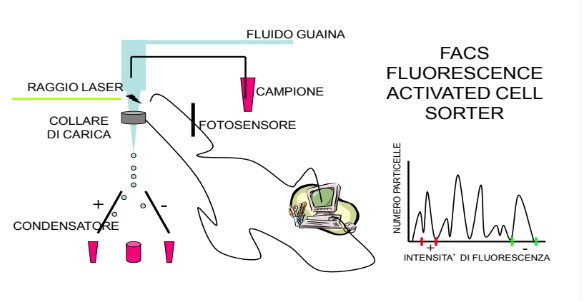
\includegraphics[width=0.6\textwidth]{img/citofluorimetro_separatore.png}
  \caption{Assetto di un citofluorimetro separatore}
\end{wrapfigure}

\textbf{Ricapitolando:} si fa questa diluizione e si tara lo strumento fino ad ottenere delle goccioline, ciascuna delle quali contiene una o piuttosto nessuna particella.\\
Ogni gocciolina viene colpita dal raggio laser, determinando l’emissione di fluorescenza.\\
Questa emissione sarà alla lunghezza d’onda opportuna, che sarà la lunghezza d’onda del fluorocromo che si è utilizzato e, se si è utilizzato semplicemente un colorante affine al DNA, avrà un’intensità proporzionale alla dimensione del cromosoma o alla quantità di DNA presente nel nucleo della cellula.

La fluorescenza emessa viene registrata da un fotosensore, a sua volta collegato ad un software che trasformerà l’informazione in linguaggio binario per poter così ottenere un grafico visualizzabile sul computer dove:
\begin{itemize}
\item sull’asse X sono riportate intensità crescenti di fluorescenza
\item sull’asse Y è riportato il numero di particelle con quella specifica intensità di fluorescenza
\end{itemize}

In particolare i cromosomi più piccoli del cariotipo saranno quelli a sinistra mentre i cromosomi più grandi del cariotipo saranno quelli a destra.

Sempre con un software di cui dispone lo strumento è possibile fare una sorta di ``gatering elettronico'', cioè stabilire delle soglie di intensità di fluorescenza.\\
Questo è possibile poiché il computer è collegato ad un collare di carica.

Nell’esempio riportato nell’immagine è stato fatto un gatering di tutte le particelle che si trovano nel picco rosso a sinistra, consentendo di separare i cromosomi che hanno quella particolare dimensione.\\
Poiché questo picco è ben isolato si stabilisce una soglia che va dalle due intensità di fluorescenza indicate dai due segmenti rossi.

Poi, per separare anche i cromosomi del picco verde a destra, cioè quelli più grandi di tutti, si fa un gatering di tutto quello che ha un’intensità di fluorescenza che va dal primo al secondo segmento verde.

Nell’esempio, si è deciso di:
\begin{itemize}
\item caricare positivamente tutte le particelle che hanno un’intensità di fluorescenza compresa nel range rosso-rosso 
\item caricare negativamente tutte le particelle che hanno un’intensità di fluorescenza compresa nel range verde-verde
\end{itemize}

Ricapitolando: le goccioline erano passate attraverso il raggio laser e ognuna di esse era stata misurata per intensità di fluorescenza ed il grafico aveva poi permesso di aprire queste due finestre elettroniche.
Poi si è ordinato al software di caricare positivamente tutto ciò compreso tra i segmenti rossi e negativamente tutto ciò compreso tra i segmenti verdi.

A questo punto quando le goccioline che rientrano nel primo range di intensità di fluorescenza passano attraverso il collare di carica vengono caricate positivamente, mentre quando rientrano nel secondo range di intensità di fluorescenza e passano attraverso il collare di carica vengono caricate negativamente.\\
Tutte le altre goccioline, che hanno un’intensità di fluorescenza che non è compresa né nella griglia verde né in quella rossa, rimarranno neutre.\\
Pertanto le goccioline, a questo punto, sono di tre tipi: positive, negative o neutre.\\
Successivamente queste goccioline cadono in mezzo alle due piastre di un condensatore, una carica positivamente e l’altra carica negativamente. Questo vuol dire che:
\begin{itemize}
\item tutte le goccioline neutre non verranno deflesse dalle piastre del condensatore cadranno nella pattumiera
\item tutte le goccioline negative, cioè quelle contenenti i cromosomi più grandi nel caso di questo esempio, verranno deflesse perché attirate dalla piastra carica positivamente e quindi cadranno in una prima provetta
\item tutte le goccioline positive verranno attirate dalla piastra carica negativamente e cadranno in una seconda provetta.
\end{itemize}

In questo modo si è ottenuta la separazione dei cromosomi del primo picco, che sono piccoli, dai cromosomi del secondo picco, che sono i più grandi di tutti.

La qualità della separazione, quindi la purezza del campione, dipende dalla qualità del grafico: quanto migliore è il grafico tanto migliore è la separazione.\\
Un grafico è tanto migliore quanto più i picchi sono separati e netti e questo dipende dallo strumento a disposizione, che può avere una sensibilità minore o maggiore.\\
È evidente che ci sarà un minimo di contaminazione, comunque irrisoria, di cromosomi un pochino più piccoli o un pochino più grandi.

Stessa cosa vale nel caso della separazione di cellule, in cui però la possibilità di purificare è migliore perché:
\begin{itemize}
\item il numero di picchi è inferiore
\item i picchi sono molto ben definiti
\item le differenze di intensità di fluorescenza sono maggiori.
\end{itemize}

Fare il sorting dei cromosomi è certamente una tecnica più sofisticata anche perché i cromosomi sono piccoli, tendono facilmente a formare grumi e a frammentarsi, quindi la purificazione non è mai del 100\%.

Il sorting è uno strumento potentissimo perché consente, nel momento in cui si ha un marcatore fluorescente, di isolare pochissime cellule in un campione, perché quelle cellule sono le uniche ad emettere fluorescenza.

Pensiamo all’importanza del sorting quando si caratterizzano i marcatori di superficie di una particolare cellula tumorale, potendo così poi marcare quelle cellule con anticorpi monoclonali specifici e magari utilizzare questi anticorpi per veicolare un farmaco contro la cellula tumorale in maniera specifica.

Il citofluorimetro a flusso separatore è utilizzato per analizzare-isolare cellule, nuclei, cromosomi, frammenti cromosomici, micro-cellule, micro-nuclei o organuli cellulari, purchè si possano marcare con un fluorocromo specifico.\\
Questo strumento può dunque essere applicato in molti settori, come la citogenetica, la citologia, l'oncologia, la diagnostica cellulare, la fisiologia cellulare, le neuroscienze.

È possibile ottenere i \textbf{cariotipi a flusso}, cioè si possono ottenere dei cariotipi semplicemente come rappresentazione dei picchi che si ottengono analizzando il preparato cromosomico di un particolare individuo. In particolare ogni popolazione di particelle con un’intensità di fluorescenza sufficientemente diversa dalle altre forma un picco separato. Questi cariotipi vengono fatti utilizzando coloranti base-specifici, ovvero coloranti che danno una colorazione che non dipende solo dalla quantità di DNA, e quindi dalla lunghezza del cromosoma, ma che dipende anche dal suo contenuto in basi, consentendo una differenziazione più dettagliata di cromosomi molto simili per dimensione. Addirittura si possono fare analisi multi-parametriche, utilizzando due coloranti diversi, uno affine alle basi AT e uno alle basi CG, aumentando così la risoluzione della separazione.\\
Tutto ciò che forma un picco distinto e netto può essere fisicamente separato in quanto goccioline contenenti particelle con una prescelta intensità di fluorescenza vengono caricate positivamente o negativamente.

Per i cromosomi i problemi sono:
\begin{itemize}
\item la contaminazione dei cromosomi piccoli con frammenti 
\item la contaminazione dei cromosomi grossi con aggregati di cromosomi più piccoli
\end{itemize} 
Per questa ragione è fondamentale la qualità del preparato iniziale.

Con strumenti ad alta separazione si arriva a distinguere particelle che presentano un coefficiente di variazione di intensità di fluorescenza anche dell’1-2\%, ovvero è sufficiente che ci sia l’1\% di diversità di fluorescenza emessa affinchè le particelle vengano risolte come picchi separati.\\

Il prezzo dello strumento aumenta a dismisura in base al numero di fasci laser presenti quindi, normalmente, gli strumenti di cui disponiamo hanno \emph{un solo fascio laser}. Pertanto sono in grado di eccitare soltanto un range limitato di lunghezze d’onda e possono essere utilizzati con un range limitato di fluorocromi.\\
I citofluorimetri più semplici lavorano con dei raggi UV, e non laser, perché non hanno bisogno di una grande risoluzione. In particolare, per risoluzione si intende la capacità di distinguere piccole differenze di intensità di fluorescenza: maggiore è la capacità di distinguere piccole differenze di intensità di fluorescenza, maggiore sarà la risoluzione dello strumento perché maggiore sarà il numero di picchi ben separati che si possono evidenziare.

\subsection{Analisi multi-parametriche}
In un’analisi multi-parametrica bisogna avere un sistema con due fasci laser, poiché si hanno due fluorocromi diversi da eccitare contemporaneamente e bisogna poter misurare la fluorescenza emessa dal fluorocromo 1 e dal fluoro cromo 2.\\

In questo caso si ottiene un’immagine di picchi che non saranno bidimensionali ma tridimensionali. In particolare:
\begin{itemize}
\item sull’asse Y viene riportato il numero di particelle 
\item sull’asse X  viene riportata l’intensità di fluorescenza del fluorocromo 1
\item sull’asse Z viene riportata l’intensità di fluorescenza del fluorocromo 2
\end{itemize}

Nelle analisi uni-parametriche (in cui, quindi, non si usano fluorocromi base-specifici e si misura semplicemente la dimensione dei cromosomi), poiché ci sono cromosomi molto simili per grandezza e quindi per contenuto di DNA, invece che ottenere 24 picchi se ne ottengono 17 poiché i cromosomi simili si raccolgono nello stesso picco.
Questo vale per i cromosomi:
\begin{itemize}
\item dal 9 al 12 (cromosomi del gruppo C)
\item dal 13 al 15 (cromosomi del gruppo D)
\item dal 21 al 22 (cromosomi del gruppo G, sono più piccoli del cariotipo umano)
\end{itemize}
Le analisi multi-parametriche invece consentono di separare tutti i cromosomi, cioè anche di distinguere i cromosomi che, normalmente, formano un picco unico.

\subsection{Riarrangiamenti strutturali e polimorfismi cromosomici}
Sfruttando riarrangiamenti strutturali e polimorfismi cromosomici è possibile, anche tramite analisi uni-paramentriche, distinguere tra cromosomi molto simili tra loro per dimensione.

Per esempio, i cromosomi dei gruppi D (13-15) e G (21-22) sono dotati di un piccolo braccio corto, chiamato mazza di tamburo e costituito da:
\begin{itemize}
\item un \textbf{peduncolo} molto sottile (l'``impugnatura della mazza di tamburo''), dove hanno sede i \emph{geni che codificano per gli rRNA}; 
\item le ``palline della mazza di tamburo'', chiamate \textbf{satelliti} (da non confondere con il DNA satellite, questi sono satelliti morfologici perché sono ``palline'' che gravitano, come se fossero dei satelliti, sul braccio corto)
\end{itemize}

Poiché questi satelliti sono altamente polimorfici per intensità di fluorescenza e presenti in maniera del tutto casuale nella popolazione, è possibile sfruttarli per distinguere, per esempio, il cromosoma 21 dal cromosoma 22.

Per fare questo si prende un individuo che ha un polimorfismo con satelliti del cromosoma 22 particolarmente fluorescenti, così che l’intensità di fluorescenza globale del cromosoma 22 sia ben diversa da quella del cromosoma 21 che, invece, non ha questi satelliti intensamente fluorescenti.\\
Stessa cosa vale per i cromosomi 13, 14 e 15.

Un altro esempio è rappresentato dai cromosomi 9, che hanno un’enorme regione di eterocromatina costitutiva che si trova subito sotto al centromero. Si tratta di una sorta di ``triangolone'' che risulta estremamente fluorescente se colorato con certi fluorocromi.\\
Questa regione è altamente polimorfica, cioè nella popolazione generale è estremamente difficile che due individui abbiano questa regione sub-centromerica del cromosoma 9 della stessa dimensione.\\
Quindi, se si usa un fluorocromo e questa regione è intensamente fluorescente, prendendo il cromosoma di un individuo che ha una particolarmente grande o particolarmente piccola regione eterocromatica del 9, si può distinguere il cromosoma 9 dagli altri cromosomi aventi dimensioni simili al cromosoma 9 (cromosomi 10, 11 e 12). Questo perché la sua dimensione finale sembrerà diversa in quanto possiede questo blocco eterocromatico intensamente fluorescente molto più grande o molto più piccolo.

Infine è possibile sfruttare le traslocazioni.

Tutto questo è importante perché, senza fare analisi multi-parametriche, sfruttando questi polimorfismi e questi particolari riarrangiamenti cromosomici, è stato possibile costruire genoteche cromosoma-specifiche, cioè è stato possibile isolare in maniera specifica tutti i cromosomi umani.\\
Queste genoteche cromosoma-specifiche di tutti i cromosomi umani isolati per chromosome sorting, sono liberamente disponibili a cifre irrisorie alla comunità scientifica internazionale dalla fine degli anni ‘90.\\

Ora vedremo l’analisi di un profilo al cell sorter dove si analizza il contenuto di DNA delle cellule.

\begin{wrapfigure}{r}{0.6\textwidth}
    \includegraphics[width=0.60\textwidth]{img/sincronizzazione_cellule.png}
  \caption{Istone H1}
\end{wrapfigure}

L’immagine nel \textbf{riquadro blu} è quello che ci si aspetta da una popolazione asincrona di \emph{cellule normali coltivate in vitro}:
\begin{itemize}
\item la maggior parte delle cellule si troverà nella fase G1, che è la fase più lunga del ciclo cellulare (la quantità di cellule in ogni fase è direttamente proporzionale alla durata di quella fase). Queste cellule costituiscono il primo picco nell’immagine in blu.
\item poi ci sarà una popolazione eterogenea di cellule con un contenuto crescente di DNA e queste saranno le cellule che stanno facendo la sintesi del DNA
\item poi ci sarà una popolazione di cellule che hanno un contenuto di DNA doppio rispetto alle cellule in G1 e, proprio per la durata delle fasi M+G2, ci si aspetta che siano di più rispetto alle cellule che sono nella fase intermedia ma che siano molte meno rispetto alle cellule che si trovano in fase G1.
\end{itemize}

Nell’immagine nel \textbf{riquadro giallo}, invece, è riportato il profilo di una popolazione di \emph{cellule sincronizzate}.\\
In particolare, le cellule sono state trattate con la \emph{colchicina}, un enzima che inibisce la polimerizzazione della beta-tubulina e che quindi inibisce la formazione del fuso mitotico, con conseguente arresto del ciclo cellulare in metafase (se non si forma il fuso le cellule non possono progredire oltre la metafase, non potendo entrare in anafase e telofase).\\
Trattando le cellule con la colchicina si ottiene un enorme arricchimento perché il numero di cellule che si trovano in M+G2, cioè cellule con un contenuto doppio di DNA rispetto alle cellule che si trovano in G1, è praticamente uguale al numero di cellule con contenuto G1 di DNA.\\
Questo è fondamentale perché se si vuole ottenere una sospensione di cromosomi isolati bisogna avere un arricchimento il più alto possibile di cellule che si trovano in metafase, per poter poi isolare i cromosomi.
 

\subsection{I cariotipi a flusso}

\begin{wrapfigure}{r}{0.68\textwidth}
    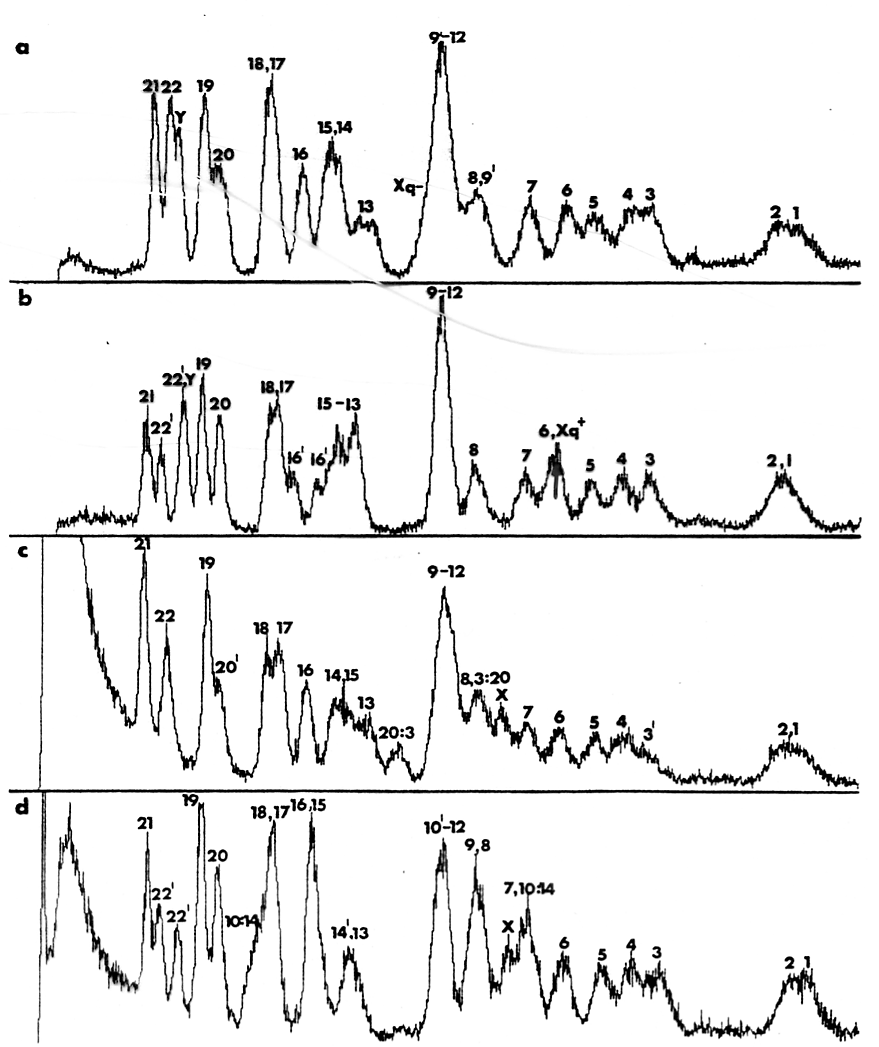
\includegraphics[width=0.70\textwidth]{img/45_cariotipo_a_flusso.png}
  \caption{Cariotipo a flusso}
\end{wrapfigure}

A destra si trovano le immagini di diversi cariotipi a flusso.\\
Si tratta di cariotipi con diversi riarrangiamenti cromosomici perché i profili sono più o meno simili ma non sono perfettamente identici. 

Nel primo caso \textbf{(a)} è possibile distinguere tra i cromosomi 21 e 22 perché, evidentemente, c’è un polimorfismo in uno di questi due cromosomi che consente di distinguerli, nonostante abbiano dimensioni molto simili.

Nel secondo caso \textbf{(b)} i cromosomi 22 e Y formano un picco solo perché c’è una traslocazione.\\
È inoltre presente un’altra traslocazione: uno dei due cromosomi X, chiamato Xq+ presenta una traslocazione del braccio lungo ed è diventato grande quanto il cromosoma 6.

Nel primo grafico \textbf{(a)}, vediamo riportato il cromosoma 9’, che si distingue dal cromosoma 9 (presente invece nel picco che va dal cromosoma 9 stesso al cromosoma 12). Questo cromosoma 9’ è più grande e ha una regione eterocromatica molto più fluorescente rispetto agli altri (discorso fatto in precedenza sul cromosoma 9).

In realtà la possibilità di fare i cariotipi in maniera automatizzata con la citofluorimetria a flusso è rimasta una pia illusione perché queste differenze non sono affidabili: ogni campione, in ogni laboratorio, è un caso a sé, non si riesce ad avere uno standard di riferimento assoluto perchè esiste una grande variabilità che dipende dal tipo di preparazione, da come è stato fatto l’isolamento dei cromosomi, da come sono condensati.\\
Questa variabilità non dipende solo dall’individuo, infatti in questo caso si ha un controllo che si sa essere perfettamente sano e che dovrebbe essere affidabile ma, ogni volta che si fa un preparato e che si isolano i cromosomi, purtroppo, c’è eterogeneità nel grado di condensazione e nella qualità della sospensione. 
Questo non permette di fare dei cariotipi automatizzati, che in realtà sarebbero un grande vantaggio, perché la citogenetica diagnostica dipende dalla perizia e dall’esperienza dell’operatore.\\
Nonostante tutte le nuove tecniche aiutino molto, non c’è una completa oggettività, c’è sempre l’operatore che deve valutare i singoli cariotipi e fare una diagnosi in base alla sua esperienza e questo, naturalmente, rappresenta un limite.

\section{La microdissezione}
Questa tecnica è usata per:
\begin{itemize}
\item identificare cromosomi o, più frequentemente, per isolare frammenti cromosomici di origine sconosciuta o anche singole bande cromosomiche
\item costruire genoteche o sonde banda o sotto-banda specifiche
\item lavorare con preparati ad altissima risoluzione in cui si riescono ad isolare dei segmenti estremamente piccoli
\item isolare regioni cromosomiche in cui sono localizzati geni malattia. In passato è stata una delle tecniche che ha permesso di clonare particolari geni malattia isolando soltanto la regione cromosomica in cui si ipotizzava fosse presente quel particolare gene malattia. Oggi, nella maggior parte dei casi, i geni malattia sono noti, sequenziati e si conoscono le mutazioni più frequenti nella popolazione.
\item  clonare microdelezioni associate a patologie costitutive o a tumori. In particolare la microdissezione può esser usata per isolare riarrangiamenti, difficilmente caratterizzabili dal punto di vista molecolare e, per esempio, coinvolti in un tumore (oggi esistono tecniche che permettono di capire, anche in riarrangiamenti molto complessi, quali siano i cromosomi coinvolti). Se si trova un punto di rottura comune a diversi tumori della stessa classe (se il riarrangiamento è causativo del cancro vuol dire che in quel punto di rottura evidentemente è successo qualcosa a carico di geni che hanno una capacità oncogena, quali oncogeni o oncosoppressori), allora riuscire a clonare esclusivamente quel punto di rottura ha una valenza enorme per poi caratterizzare i geni presenti a livello del punto di rottura, che devono essere evidentemente coinvolti o nell’eziologia o nello sviluppo o nella progressione del tumore.
\end{itemize}
 
Questa tecnica è riservata a citogenetisti molecolari con grande esperienza perché vuol dire lavorare al microscopio ottico rovesciato facendo micromanipolazione e prelevando singoli frammenti da singole cellule metafasiche che devono essere preparate con particolari metodologie.

In realtà oggi è sufficiente prelevare 5-10 frammenti cromosomici, perché ci sono delle tecniche di microamplificazione e microclonaggio.\\
Si parla di picogrammi di DNA ma, grazie a delle tecniche ad hoc, è possibile lavorare in microvolumi, amplificarli e purificarli, riuscendo ad avere poi una quantità di DNA sufficiente per le applicazioni diagnostiche.

Il DNA cromosomico viene amplificato in vitro (PCR) con primer Alu o primer degenerati.

Fare una microdissezione bene vuol dire identificare il cromosoma e prelevare esclusivamente la banda o la microbanda che si deve isolare. In questo caso la purezza del campione è vicina al 100\% e si tratta esclusivamente di DNA umano.\\
Per amplificare è possibile fare una Alu PCR perché, essendo sequenze ripetute intersperse, si amplifica tutto.\\
Le sequenze LINE e SINE tuttavia non sono uniformemente distribuite nel genoma (le LINE hanno la tendenza a localizzare nelle regioni intergeniche mentre le SINE nelle regioni geniche), quindi, se si fa una Alu PCR, in realtà, si fa un’amplificazione selettiva delle regioni che contengono geni.\\
Oggi è addirittura quasi più importante amplificare le regioni che non contengono geni perché sono quelle che contengono i segnali regolativi.

Pertanto, dato che in questo caso non serve la specie-specificità, si possono usare i \textbf{primer degenerati}.
Questi sono \emph{costruiti con dei programmi di randomizzazione} in modo da amplificare un po’ qualsiasi cosa, cioè in modo da essere rappresentativi di qualsiasi sequenza nel genoma.\\
I primer degenerati non si possono usare negli ibridi somatici perché verrebbe amplificato anche il genoma di topo, dovranno essere invece utilizzati dei primer specie-specifici.

Generalmente, per esempio quando si fa la microiniezione, è necessario usare un micromanipolatore sinistro, per tenere ferma la cellula, ed un micromanipolatore destro, che, con una pompa peristaltica, preleva quello che c’è da iniettare e lo inietta nella cellula bersaglio grazie a un microcapillare (questa tecnica è usata, per esempio, nel caso di  trapianti di nuclei in ovociti per fare fecondazione in vitro).\\
In questo caso, invece, siccome i cromosomi sono fissati sul vetrino, è sufficiente avere il micromanipolatore destro, che è mosso da una cloche, che permette di fare micromovimenti ed è collegato ad un capillare il più sottile possibile che funziona come se fosse un cucchiaino.\\
Per avere i capillari il più sottile possibile li si mette sopra la fiamma, li si tira a mano e li si spezza.
In questo modo il capillare sarà sottilissimo ed il punto di rottura non sarà netto ma storto e questo fa in modo che funzioni proprio come un cucchiaino di piccolissime dimensioni.\\
Questo verrà utilizzato per fare uno ``scraping'' (raschiamento) del pezzettino di interesse.

Naturalmente se si deve prelevare un segmento di un particolare cromosoma che corrisponde ad una particolare interbanda, i cromosomi devono essere fissati, colorati e bandeggiati e questa è la cosa più complicata: bisogna fare dei preparati cromosomici fissando per tempi brevi, per non depurinare completamente il DNA, e colorando ad hoc le singole metafasi.\\
La cosa sofisticata è soprattutto questa ed è riservata agli esperti di citogenetica.\\
Comunque, in questo modo, si avranno singole cellule fissate sul vetrino, colorate e bandeggiate e poi si andrà a fare questo lavoro di microdissezione di singole bande o di singoli segmentini.

Un altro modo per fare microdissezione è quello della \textbf{microdissezione laser}, che però è molto meno precisa. In particolare, l’uso dei laser consente di lasciare sul vetrino solo quello che interessa, infatti si parla di \textbf{ablazione laser}, perché il laser distrugge tutto quello che non interessa.\\
Questa tecnica può andare bene per intere cellule, ma nel caso di una banda cromosomica la microdissezione meccanica è la migliore.

Una volta fatta la microdissezione, si procede alla microamplificazione.
In particolare, si ha il vetrino dove si hanno le singole metafasi fissate e colorate e su cui si è fatta la micromanipolazione meccanica e, sullo stesso vetrino, a fianco, si costruisce artigianalmente una cameretta, cioè un microvolume, per fare direttamente la PCR dei segmentini.

Fondamentalmente, si fa una sorta di cilindretto, ottenuto tagliando delle provette usate generalmente per congelare (diametro di poco inferiore a mezzo centimetro) e lo si appiccica con il silicone. In questa sorta di camera si mette un goccio di olio di paraffina, che diventa il microvolume dove si andranno a mettere i pezzettini che sono stati prelevati tramite micromanipolazione meccanica e in cui si faranno le reazioni di PCR che, inizialmente, vengono fatte con quantità piccolissime di DNA.\\
Chiaramente tutti i passaggi verranno fatti per diluizione (non si può centrifugare) e quindi bisogna scegliere enzimi che lavorano in tamponi compatibili perché non si può purificare il DNA estratto centrifugando e, ogni volta, bisognerà aggiungere un tampone diverso.

\textbf{Riassumendo:} lavorando al microscopio vedo che sul cucchiaino si ha il pezzettino di cromosoma, lo si trasferisce nella cameretta, lo si mette nella goccia di paraffina, si aspetta che si stacchi, se ne prende un altro, lo si mette nella goccia di paraffina e si aspetta che si stacchi. Alla fine si avranno n frammentini nella goccia di paraffina. A questo punto si potrà procedere con le altre reazioni, inizialmente in questo microvolume e poi, dopo aver fatto l’amplificazione, si potrà lavorare in volumi più grossi.

Tramite microdissezione sono stati isolati e clonati 7 geni malattia diversi.
È evidente che sia una tecnica sofisticata e riservata a pochissimi laboratori ma poiché la purezza del frammento è quasi pari al 100\%, l’isolamento del gene è molto affidabile.

Tramite microdissezione è anche possibile identificare un cromosoma marcatore tumorale: si isola il punto di rottura e lo si usa come sonda in una sorta di reverse chromosome painting, cioè si usa il segmento di giunzione del punto di rottura per andare sui cromosomi normali e vedere quali sono i cromosomi da cui deriva il cromosoma marcatore tumorale che non si riusciva ad identificare.
Si parla di reverse chromosome painting perché si usa il marcatore come sonda per identificare se stesso.


\subsubsection{A cosa servono i cromosomi isolati?}
\begin{enumerate}
\item per la \textbf{costruzione di genoteche cromosoma specifiche}, cioè è possibile avere una quantità di DNA clonata in plasmidi, che è possibile continuare ad amplificare potendo conservare, tramite congelamento, il DNA di quel cromosoma per tutta la vita
\item per la \textbf{produzione di painting probes} (chromosome painting), di cui abbiamo parlato per la loro funzione nell’ibridazione in situ
\item per l'\textbf{identificazione di riarrangiamenti cromosomici complessi nel cancro}
\item per l'\textbf{identificazione di marcatori cromosomici}, non diversamente identificabili, attraverso reverse chromosome painting
\item per l'\textbf{identificazione di micro-cromosomi}
\item per l'\textbf{identificazione di micro-riarrangiamenti}
\item per l'\textbf{analisi comparata di cariotipi} (Comparative Chromosome Painting): se si vuole sapere, per esempio, quale sia la storia evolutiva del cromosoma 1 umano, si prende il cromosoma 1 isolato e lo si va ad ibridare in specie sempre più lontane, usando delle condizioni di ibridazione sempre più permissive man mano che ci si allontana dall’uomo.
In questo modo è possibile sapere quali segmenti cromosomici si sono riarrangiati nel corso dell’evoluzione dei cariotipi. Questi approcci di comparative chromosome painting hanno permesso di avere un ipotetico cariotipo ancestrale di tutti i Vertebrati.
\end{enumerate}


\section{Le genoteche cromosoma specifiche} 
Una volta che si estrae e si purifica il DNA dal cromosoma isolato, esso viene tagliato e inserito in dei vettori.\\
I vettori da utilizzare dipendono dalle dimensioni dei frammenti isolati e potranno essere YAC, BAC o plasmidi.\\
L’ideale sarebbe avere dei BAC ma, in generale, è più facile avere delle genoteche in cui i segmenti sono clonati in vettori plasmidici.

Le genoteche cromosoma specifiche sono insostituibili per isolare geni malattia perché sono una fonte arricchita soltanto di sequenze che riguardano la regione cromosomica di interesse.\\
Esempi in cui, grazie all’isolamento di frammenti cromosomici, si è arrivati all’identificazione dei geni malattia sono:
\begin{itemize}
\item sindrome dell’X fragile; 
\item neurofibromatosi II; 
\item sindrome Di George; 
\item micromarcatori cromosomici; 
\item punti di rottura in microriarrangiamenti alla base di malattie e tumori; 
\item double minutes e regioni HSR nei tumori. Queste sono zone amplificate, di diverso tipo, nel cancro. Quindi è stato fondamentale capire quale fosse il gene che amplificandosi determinasse lo sviluppo del cancro. Un esempio è il cancro alla mammella, in cui la progressione è direttamente collegata all’amplificazione genica.
\end{itemize}

\subsubsection{Il Chromosome Painting}
Il ``chromosme painting'' (pittura dei cromosomi) è un tipo di FISH con competizione che utilizza come sonda interi cromosomi o segmenti cromosomici precedentemente isolati.\\
Il cromosoma isolato viene amplificato per PCR (con primer degenerati, ALU o sequenze ripetute intersperse specie-specifiche).\\
I frammenti amplificati vengono marcati mediante nick-translation e il DNA marcato viene denaturato e miscelato con un largo eccesso di DNA genomico totale denaturato non marcato (DNA competitore) della specie alla quale appartiene il cromosoma di interesse.\\
Il DNA competitore essendo DNA genomico è costituito prevalentemente da sequenze altamente ripetute che hanno una velocità di rinaturazione altissima, quindi satura tutte le sequenze ripetute presenti nella sonda.\\
Dopo competizione sono disponibili per l’ibridazione successiva solo le parti di DNA sonda che non sono state saturate dal competitore ossia le sequenze a singola copia.
Il DNA sonda così preparato viene ibridato a preparati cromosomici adatti.

Questa tecnica viene utilizzata per:
\begin{itemize}
\item Identificazione di cromosomi marcatori:
	\begin{itemize}
	\item Il cromosoma marcatore isolato costituisce la sonda;
	\item Il bersaglio è rappresentato da un preparato di cromosomi metafasici, prometafasici o profasici normali;
	\item Si pitturano tutti i segmenti cromosomici dai quali deriva il cromosoma marcatore.
	\end{itemize}

\item Identificazione di micro-cromosomi:
	\begin{itemize}
	\item Il micro-cromosoma isolato costituisce la sonda;
	\item Il bersaglio è rappresentato da un preparato di cromosomi metafasici, prometafasici o profasici normali;
	\item Si pittura il segmento cromosomico dal quale deriva il micro-cromosoma.
	\end{itemize}

\item Definizione dei punti di rottura di riarrangiamenti complessi:
	\begin{itemize}
	\item Il punto di giunzione di un riarrangiamento complesso viene isolato e costituisce la sonda;
	\item Il bersaglio è rappresentato da un preparato di cromosomi metafasici, prometafasici o profasici normali;
	\item Si pitturano i segmenti cromosomici contenenti il punto di rottura.
	\end{itemize}

\item Comparative chromosome painting:
	\begin{itemize}
	\item Un cromosoma o un segmento cromosomico isolato di una certa specie costituisce la sonda;
	\item Il bersaglio è rappresentato da un preparato di cromosomi metafasici, prometafasici o profasici normali di una specie diversa;
	\item Si pitturano i cromosomici sintenici al cromosoma (segmento cromosomico) di partenza.
	\end{itemize}
\end{itemize}



\chapter{La regolazione dell'espressione genica}
Quando si parla di ``regolazione dell’espressione genica'' ci si riferisce a tutto quello che può succedere a partire dalla sequenza di DNA fino ad arrivare alla proteina matura.\\
Quello della regolazione dell’espressione genica è un campo infinito che include diverse branche della biologia. I due esempi modello storici, quello dei cromosomi politenici (fenomeno del puffing) e dei cromosomi a spazzola, sono esempi di regolazione epigenetica e di modificazione locale della cromatina.\\
Noi parleremo dettagliatamente del fenomeno della \textbf{compensazione del dosaggio genico} usando due esempi che rappresentano due modi opposti per risolvere lo stesso problema biologico:
\begin{itemize}
\item l’inattivazione funzionale del cromosoma X nei mammiferi (il primo modello approfondito di regolazione epigenetica dell’espressione genica)
\item la compensazione dei geni legati all’X attuata in Drosophila.
\end{itemize}

In C. elegans c’è ancora un diverso meccanismo epigenetico di compensazione del dosaggio che è all’interfaccia tra quello utilizzato nei mammiferi e quello utilizzato nella Drosophila.

Infine parleremo di \textbf{imprinting genomico}, che negli anni '90 ha rivoluzionato il modo di vedere i meccanismi di regolazione dell’espressione genica.


\section{I livelli di controllo dell'espressione genica}
I livelli di controllo possibili sono molti e molto diversi: alcuni agiscono nel nucleo, altri nel citoplasma dopo che l’RNA è stato esportato, ecc; dovunque sia coinvolto un processo metabolico che prevede l’azione di enzimi ci può essere un livello di controllo.

Il primo livello di controllo che interessa i genetisti avviene a livello del DNA ed è il \textbf{controllo della trascrizione} (è quello energeticamente più ``economico'' per la cellula).\\
Questo controllo avviene attraverso l’azione combinata di specifiche sequenze regolatrici: il primo modello scoperto per la regolazione dell’espressione genica è stato il \textbf{modello dell’operone} scoperto nei batteri, modello che poi si è capito adattarsi molto poco negli eucarioti nei quali la struttura genomica è più complessa. Questo modello è stato comunque fondamentale per l’identificazione di sequenze chiave che regolano l’espressione genica, ovvero promotori e sequenze che interagiscono con gli elementi regolativi (i.e. induttori e repressori).

Esistono mutanti, detti \emph{``costitutivi''}, che non risentono degli elementi regolativi (induttori o repressori) perché possiedono delle mutazioni nella sequenza del promotore; tanti altri casi sono ben noti nelle patologie umane in cui alterazioni dell’espressione genica sono dovute ad alterazioni della sequenza di elementi regolativi. 

La maggior parte della regolazione dell’espressione genica è però dovuta a \textbf{meccanismi di tipo epigenetico}: questi sono meccanismi che non alterano la sequenza del gene, tantomeno del promotore o degli effettori che agiscono sul promotore (o su enhancers e silencers), ma sono delle modificazioni biochimiche che possono avvenire a livello del DNA (e.g. metilazione di specifiche citosine, modificazioni chimiche a livello degli istoni con conseguente modificazione della struttura del DNA e del nucleosoma) e che possono essere attivanti o inattivanti. Le modificazioni epigenetiche consistono in \textbf{modificazioni post traduzionali} degli istoni che possono ad esempio essere acetilati, o nella metilazione di particolari residui istonici. Questi avvenimenti modificano il grado di condensazione della cromatina, di impacchettamento dei cromosomi, nascondendo o esponendo sequenze regolative o addirittura modificando il territorio cromosomico o il dominio cromatinico in cui si trova un certo gene che così può essere lasso o ipercondensato, e in questo modo essere attivato o inattivato.

Questo è il meccanismo principe di controllo della trascrizione negli eucarioti.

Gran parte del genoma non viene tradotta ma solamente trascritta in RNA che possono essere long non coding RNAs e short non coding RNAs: ognuno di essi ha un ruolo diverso nella regolazione dell’espressione genica.

I trascritti primari normalmente sono soggetti a maturazione e splicing: anche questi passaggi possono essere controllati. La stragrande maggioranza dei geni è soggetta a splicing alternativo, ovvero a seconda di quali introni vengono rimossi o meno, una stessa sequenza può esprimere proteine diverse che possono avere non solo funzioni diverse ma anche una diversa tessuto-specificità.\\ Tutto questo avviene ancora all’interno del nucleo.

Una volta maturato, il trascritto deve essere esportato dal nucleo per entrare nel citoplasma dove sono presenti ulteriori elementi di controllo: può essere controllato il trasporto (è un evento attivo, per cui l’efficienza con cui il trascritto viene esportato è modulabile), oppure la stabilità dei messaggeri (il turn-over). Anche nel controllo della stabilità dei messaggeri hanno un peso rilevante molecole di RNA non tradotti.

La traduzione, visto quanti sono gli elementi che intervengono nel processo, è fortemente controllata, ma anche in seguito alla formazione della proteina questa può essere ulteriormente processata, modificata attraverso chinasi o altri fattori che possono poi regolarne l’attività. C’è un numero enorme di elementi che intervengono simultaneamente o separatamente.

Per quanto riguarda il flusso delle vie metaboliche che portano all’attivazione di una particolare rete di reazioni, in genere il meccanismo è questo: ogni volta che abbiamo una via metabolica strettamente controllata durante lo sviluppo e il differenziamento, c’è una sequenza di interruttori che accendono o spengono diverse ramificazioni di questa via metabolica, fino ad arrivare a una rete complessa di vie metaboliche più o meno interconnesse tra loro. Il principio è quello di una sequenza gerarchica di interruttori che se accesi o spenti danno la possibilità di progredire verso ramificazioni successive di una via metabolica principale che si suddividerà in vie secondarie che a loro volta si ramificheranno in due o più vie metaboliche di ordine superiore e via dicendo. Alla fine si avrà una rete di vie metaboliche che porteranno allo sviluppo e al differenziamento. Abbiamo un punto di partenza, un interruttore principale che se acceso andrà ad accendere e/o spegnere una via metabolica.

\begin{wrapfigure}{r}{0.6\textwidth}
    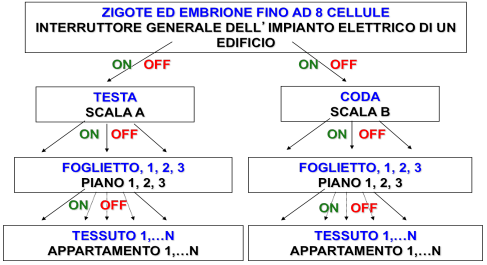
\includegraphics[width=0.6\textwidth]{img/impianto_elettrico.png}
  \caption{Il differenziamento cellulare}
\end{wrapfigure}

Prendiamo come esempio esplicativo l’impianto elettrico di un grande edificio: se partiamo dalla situazione indifferenziata (lo zigote fino allo stadio di 8 cellule totipotenti) abbiamo un interruttore generale che accende/spegne l’impianto elettrico di tutto l’edificio. Si avrà un primo livello di differenziamento, che è il commitment di una parte delle cellule a disegnare l’asse cefalo-caudae, abbiamo dunque una prima biforcazione in due vie metaboliche ben distinte, chiamate in figura scala A e scala B. C'è una parte delle cellule che segue una via metabolica per cui sono committed, destinate, a formare la testa, mentre quelle della scala B sono destinate a formare la coda.\\
Ci sono poi altri interruttori che possono essere accesi o spenti e a seconda di questo determinano i diversi abbozzi dei foglietti che poi origineranno i diversi tessuti e questo vale sia per le cellule della scala B che per le cellule della scala A che sono già committed. In figura è rappresentato come il livello di regolazione dell'accensione o dello spegnimento dell’impianto elettrico ai diversi piani di questo edificio. Ad ogni piano, ogni appartamento potrà avere o meno l’impianto elettrico acceso o spento, e quindi di nuovo degli interruttori che differenzieranno all’interno di ciascun foglietto i diversi tessuti, e cioè la luce arriva ai diversi appartamenti fino ad arrivare al poter accendere o spegnere la abat-jour del proprio comodino.
Dobbiamo sempre pensare a un ordine gerarchico di interruttori fino a formare una rete: vie metaboliche estremamente interdigitate tra loro.

Le modificazioni epigenetiche consistono in cambiamenti della cromatina che regolano l’espressione genica a livello trascrizionale negli eucarioti.
Le modificazioni epigenetiche non alterano la sequenza del DNA, ma solo la struttura tridimensionale della cromatina.

La domanda sorge spontanea: queste modificazioni che non riguardano la sequenza del DNA sono ereditabili per via mitotica? Sì, esiste una memoria cellulare. Ma sono ereditabili per via germinale? E se sì, quanto? Questo problema mette in discussione concetti a un livello molto avanzato. È una sorta di neo-lamarckismo. È evidente che se si parla di modificazioni indotte dal cambiamento della cromatina è perché ci sono dei segnali ambientali durante lo sviluppo e il differenziamento (stimoli interni che cambiano la risposta della cellula e ne determinano il cambiamento funzionale quali ormoni o fattori regolativi). Questi segnali possono essere modificati e indotti da elementi fisici. In questo caso non si parla di cambiamenti acquisiti come nel lamarckismo classico (caratteristiche non ereditabili come il collo lungo della giraffa), ma siccome l'RNA può essere retro-trascritto in alcuni casi è stato dimostrato che nella sequenza del DNA vengono introdotte delle modificazioni che poi saranno ereditate anche nella progenie. Sono argomenti di dibattito molto interessanti. Non mettiamo in dubbio il modo di pensare l’evoluzione, però introduciamo nozioni che cambiano il modo di vedere l’eredità dei caratteri acquisiti anche se non riguardano fenotipi eclatanti come la lunghezza del collo.

I cambiamenti epigenetici hanno un ruolo chiave nei processi di regolazione dell’espressione genica negli eucarioti.\\
Le modificazioni epigenetiche non riguardano le sequenze regolatrici per sé, ovvero promotori, enhancers o silencers, ma piuttosto l’accessibilità di tali sequenze ai fattori con cui queste interagiscono.

Le modificazioni epigenetiche consistono in:
\begin{itemize}
\item metilazione delle citosine del DNA,
\item metilazione ed acetilazione di specifici gruppi istonici che formano l’ottamero del nucleosoma. 
\end{itemize}

C’è un equilibrio locale nelle regioni del genoma tra gruppi di metili e gruppi di acetili, e quando questo rapporto raggiunge un valore critico si ha attivazione o repressione dell’espressione genica. Dal momento che localmente nei genomi c’è un rapporto ben specifico che varia nel tempo, si parla di \textbf{codice istonico}. A causa della sua plasticità decodificare questo codice risulta difficile: varia tra le cellule dell’organismo in funzione del grado di sviluppo e differenziamento, ma anche in funzione del ciclo cellulare.

Durante la trascrizione e la replicazione la doppia elica di DNA si deve aprire per essere accessibile al complesso trascrizionale o al complesso replicativo, gli istoni si staccano, il nucleosoma si distrugge per poi riformarsi non appena completato il processo. La cromatina deve essere in una conformazione adatta affinché si stacchino gli otto istoni che formano il nucleosoma. Poi, appena completato il processo di trascrizione o di replicazione, gli istoni dell’ottamero si riassociano al DNA. Tutto questo è modulato dal grado di condensazione della cromatina. Nel modello del nucleo interfasico, la cromatina ha una struttura ad anse. Esistono meccanismi che modulano il grado di condensazione delle anse, e anche la loro dimensione. Le anse sono più o meno compatte in diversi momenti funzionali e in diverse regioni cromosomiche.

Come già descritto nel capito 3, la cromatina può essere suddivisa in \emph{eterocromatina} ed \emph{eucromatina}.

Ricordiamo che le caratteristiche dell'\textbf{eterocromatina} sono:
\begin{itemize}
\item rappresentano regioni del cromosoma eucariotico \emph{dense e compatte} in telofase, interfase e prima profase
\item sono più \emph{intensamente colorate} in tutte le fasi del ciclo cellulare
\item si divide in:
	\begin{itemize}
		\item \textbf{Costitutiva:} queste sono regioni specifiche di cromatina costituzionalmente (i.e. sempre) eterocromatiche, presenti su ambedue gli omologhi in tutti i tipi cellulari e in tutti gli stadi dello sviluppo (con le eccezioni che confermano la regola)
		\item \textbf{Facoltativa:} sono regioni eterocromatiche soltanto in alcune cellule o in alcuni organismi, oppure lo sono solo in alcuni individui della stessa specie. Può succedere anche che un omologo sia eterocromatico e l’altro no. Sono porzioni di eterocromatina localizzate in regioni cromosomiche che normalmente sono eucromatiche. Due esempi sono:
				\begin{itemize}
					\item i cromosomi paterni nei maschi di alcune specie di insetti in cui vi è ipercondensazione e inattivazione funzionale di tutto il set cromosomico paterno che determina lo sviluppo in senso maschile,
					\item il cromosoma X inattivo nelle femmine dei mammiferi. Nei maschi dei mammiferi c’è un solo cromosoma X e nella donna 2: uno è ipercondensato e l’altro no. Questo processo riguarda solo i tessuti somatici delle cellule dei mammiferi (riguarda solo un omologo, in modo diverso tra i diversi tessuti) mentre per lo sviluppo dei gameti è ovvio che devono essere attivi entrambi.
                  \end{itemize}
	\end{itemize}
\item sono \textbf{allocicliche} (hanno un ciclo di replicazione diverso, in larga misura sono a \emph{replicazione tardiva})
\item sono ritenute in larga misura \emph{geneticamente inerti}.
\end{itemize}

Le ultime due affermazioni non sono esattamente vere, infatti lo studio ad alta risoluzione dei genomi ha dimostrato l'esistenza di sotto-territori attivamente trascritti e meno condensati all'interno delle regioni eterocromatiche.

Le caratteristiche dell'\textbf{eucromatina} invece sono:
\begin{itemize}
\item regioni del cromosoma eucariotico che subiscono il \emph{normale ciclo di condensazione}
\item a \emph{colorazione pallida} in tutte le fasi del ciclo (se uso un colorante come il ghilsa o una colorazione citologica, sono meno elettrondense al microscopio elettronico)
\item si pensa che contengano i geni funzionalmente attivi
\end{itemize}

\section{La compensazione del dosaggio genico}
Nelle specie con cromosomi del sesso eteromorfi (i.e con morfologia diversa – esistono modelli diversi quali x0 o zw) ed in particolare nelle specie a determinazione cromosomica del sesso di tipo XX/XY, tutti i geni localizzati sul cromosoma X sono in doppia dose nelle femmine. 

Tutte le volte che c’è eteromorfismo dei cromosomi del sesso il dosaggio genico delle sequenze è diverso, ma le cellule somatiche di maschi e femmine di qualsiasi specie devono essere metabolicamente uguali. C’è una differenza di dose genica come sequenza, che deve essere compensata perché si deve avere un’identica dose di prodotto genico.
 
Sia in Drosophila che nell'uomo il cromosoma X è molto grande mentre l’Y è piccolo. Inoltre molti dei geni localizzati sul cromosoma X sono geni house-keeping, mentre il cromosoma Y è prevalentemente eterocromatico e privo di geni, a parte una piccola porzione che contiene geni legati allo sviluppo dei caratteri sessuali secondari, alla fertilità, e necessari per lo sviluppo in senso maschile della gonade indifferenziata. La gonade indifferenziata è un ovario rudimentale che, per svilupparsi in quella maschile, necessita dell’attivazione di geni sul cromosoma Y.

Nelle cellule somatiche di organismi maschili e femminili dunque, a causa delle differenze tra i due tipi di cromosomi, vi sarà una differenza nella quantità di prodotto genico del cromosoma X. Questa differenza deve essere annullata in quanto le cellule somatiche devono essere uguali. I meccanismi che portano a questa uguaglianza di dose di prodotto nelle cellule somatiche femminili e maschili prendono il nome di \textbf{``compensazione del dosaggio dei geni legati all’X''} e sono modificazioni di tipo epigenetico.

Questo è un classico esempio di come nell’evoluzione uno stesso problema biologico sia stato risolto in modo diverso in specie diverse (convergenza evolutiva). Questi meccanismi si basano sempre e comunque su meccanismi di regolazione epigenetica.

Nei \textbf{mammiferi} il meccanismo di compensazione si basa sull’inattivazione funzionale di uno dei due cromosomi X in tutte le cellule somatiche femminili. Questo avviene fondamentalmente attraverso la \emph{metilazione del DNA}. \\
Nella \textbf{Drosophila} invece si ha un meccanismo opposto, perché si ha una iper-espressione dei geni localizzati sull’unico cromosoma X maschile.
In questo caso la base molecolare è l’\emph{acetilazione dell’istone H3} dei nucleosomi del cromosoma X maschile. 

La determinazione del sesso nei mammiferi dipende dalla presenza dell’Y, in particolare dalla presenza di quelle sequenze dove ci sono i determinanti per il differenziamento della gonade in senso maschile. Nella Drosophila invece, a determinare il sesso dell'organismo, è il rapporto tra il numero intero di set di autosomi e il numero di cromosomi X. Quando vi è un rapporto di 1:1 (2 set autosomi e 2 cromosomi X) lo sviluppo è in senso femminile, mentre quando il rapporto è di 1:2 lo sviluppo è in senso maschile. Esistono inoltre delle forme di \emph{intersesso} dovute a rapporti cromosomici diversi rispetto a quelli appena descritti.

È grazie alla scoperta del \textbf{corpo di Barr} che è stato subito facile fare un’ipotesi su quale fosse il meccanismo di compensazione del dosaggio genico nei mammiferi. La completa delucidazione del meccanismo molecolare della compensazione del dosaggio è arrivata intorno alla fine degli anni '90.\\
A tutt’oggi comunque ci sono ancora una grande quantità di quesiti aperti sul meccanismo molecolare che permette la compensazione.
Sappiamo che nei mammiferi intervengono dei meccanismi basati sull’intervento di molti RNA non tradotti.\\

\subsection{L'inattivazione funzionale del cromosoma X}
Per comprendere come si sia arrivati a questa scoperta seguiamo il percorso storico della maturazione del pensiero scientifico.

\begin{enumerate}
\item \textbf{Osservazioni morfologiche} del corpo di Barr: già tramite queste risultò chiaro che il meccanismo di inattivazione dipendesse da una ipercondensazione del DNA
\item \textbf{Osservazioni citologiche}
\item \textbf{Osservazioni genetiche} basate su cosa sull-osservazione del fenotipo in incroci e nella progenie di individui che hanno anomalie dei cromosomi del sesso
\item \textbf{Ipotesi di Mary Lyon}, la quale altro non è che la sintesi delle osservazioni precedenti 
\item \textbf{Prove citologiche}
\item \textbf{Studio dei marcatori genetici}
\item \textbf{Studio del meccanismo molecolare}
\end{enumerate} 

Per la prima volta nel 1949 Barr osserva in nuclei interfasici di cellule somatiche di femmine di gatto la \textbf{cromatina sessuale}. Questa è visibile come un corpo eterocromatico più intensamente colorato rispetto al resto dell’eterocromatina, associato alla membrana nucleare (è una pallina molto scura che si osserva solo nelle cellule femminili somatiche).

Successivamente venne osservato che tutti i nuclei interfasici di cellule somatiche normali di femmine di mammifero presentano un corpo di Barr.

Lo studio delle patologie legate al corpo di Barr avviene almeno 10-15 anni dopo la sua scoperta (all’epoca lo studio delle patologie era fatto principalmente sull’uomo).\\
I \emph{riarrangiamenti del cromosoma X} sono molto frequenti ma, nella maggior parte dei casi, hanno un blando effetto fenotipico. Si parla di anomalie strutturali, traslocazioni, piccole delezioni e via dicendo.

Queste anomalie possono influenzare lo sviluppo e la fertilità ma solitamente non portano a patologie gravi: non sono dunque clinicamente rilevanti e sono piuttosto frequenti nella popolazione perchè compatibili con la vita.\\
Se facciamo un’analisi delle anomalie dei cromosomi del sesso nell’uomo vediamo che c’è una correlazione tra il numero di corpi di Barr ed il numero di cromosomi X attivi. Questa è la \textbf{regola dell’N1}: indipendentemente dal numero di cromosomi X presenti nella cellula ne verrà sempre mantenuto \emph{uno solo} attivo. Questo fenomeno riguarda i casi di trisomie, tetrasomie e addirittura pentasomie X: queste sono femmine normali, con un lieve ritardo mentale in alcuni casi, e sono femmine che hanno un’alta probabilità di avere figli con la \textbf{sindrome di Klinefelter} perché può segregare in un gamete più di un cromosoma X (Klinefelter: \emph{cariotipo 47-XXY}). 

Nella \textbf{sindrome di Turner} invece il cariotipo è \emph{X0}. Osservando la cromatina sessuale in un individuo con la sindrome di Klinefelter osserveremo una cromatina di tipo femminile, mentre se si osserva la cromatina sessuale in una femmina Turner questa presenterà una cromatina di tipo maschile perché non avrà il corpo di Barr. Nelle diagnosi prenatali per la determinazione del sesso si analizzava la cromatina sessuale, dunque queste patologie sfuggivano alle analisi.

In presenza di anomalie strutturali del cromosoma X viene preferenzialmente inattivato il cromosoma X riarrangiato. 
Questo è molto utile perché se ho una femmina con un cromosoma X deleto e quello viene inattivato avrò una femmina con un fenotipo Turner parziale (è un fenotipo molto vicino a quello normale), mentre se venisse inattivato l’X normale si avrebbe una grave patologia.

L’inattivazione normalmente è casuale, ma perché in questi casi non è così? Dobbiamo pensare a un meccanismo di selezione darwiniana: i soggetti con questa patologia che inattivano l’X riarrangiato crescono meglio e di conseguenza hanno maggiori possibilità di riprodursi.

Nel 1950 la dott.ssa Russel fece delle analisi fenotipiche su femmine di topo tramite costruzione di traslocazioni ad hoc di geni che determinano il colore del mantello sul cromosoma X (il risultato erano femmine con il fenotipo del mantello variegato, a chiazze): se i geni sono traslocati sull’X e l’inattivazione è casuale, a seconda dell’X inattivato l’animale avrà un colore diverso del mantello.\\
Questa è un’evidenza indiscutibile del fatto che uno dei due cromosomi X viene inattivato nelle cellule somatiche e ci dice che l’inattivazione è casuale infatti il mantello risulta a chiazze, perché in ogni cellula può essere inattivato l’uno o l’altro cromosoma a caso.\\
Non solo, ma che tutta la progenie mitotica (ho una chiazza, una regione di cellule epidermiche) ha una sorta di memoria cellulare. Una volta fatta la scelta tutta la progenie mitotica avrà sempre quel cromosoma X inattivo.

Un altro esempio è quello dei \textbf{``gatti tartaruga''} o \textbf{``gatti calico''} e di femmine di topo eterozigoti. Le femmine di \emph{gatti calico} eterozigoti per un gene legato all’X (non è una traslocazione come nel caso della Russel) che determina il colore del mantello sono a chiazze. Ovviamente, se guardiamo la progenie di queste femmine, i maschi non risultano mai a chiazze ma abbiamo un 50\% di maschi con il pelo di un colore e un 50\% dell’altro.

L’\textbf{ipotesi di Mary Lyon} è la sintesi di tutto quello che abbiamo detto e può essere riassunta così: \emph{caratteri legati al sesso mostrano variegazione o mosaicismo somatico nelle cellule somatiche delle femmine eterozigoti}.

Nella sua ipotesi Mary Lyon affermò che:
\begin{itemize}
\item a compensazione del dosaggio nei mammiferi avviene attraverso l’inattivazione di uno dei cromosomi X presenti nelle femmine. Si ottiene in questo modo l’equivalenza funzionale dei geni posti sul cromosoma X nei maschi e nelle femmine.
\item può essere inattivato a caso l’X materno o quello paterno (ci sono eccezioni all’inattivazione casuale già citate)
\item l’inattivazione, nel topo, avviene in uno stadio precoce dello sviluppo embrionale (5 gg dopo la fecondazione nel topo, nell’uomo avviene dopo più tempo)
\item l’inattivazione viene ereditata somaticamente: le cellule derivate per mitosi da una cellula con inattivato l’X materno hanno sempre inattivato l’X materno e viceversa. Questo fenomeno viene detto di \textbf{memoria cellulare} e spiega il mosaicismo.
\end{itemize}

Il cromosoma X inattivo, a causa della sua ipercondensazione, è l’ultima regione del genoma che si replica durante la fase S. Il corpo di barr viene chiamato anche \textbf{inactive X (iX)} o \textbf{late X (lX)}.\\
Questo si vede bene con l’incorporazione di trizio o bromodesossi uridina in fase S, un tracciante che si vede bene con anticorpi o colorazioni differenziali.
Facendo l’incorporazione di timidina poi con autoradiografia si vede che il cromosoma X incorpora
molto più trizio rispetto a tutti gli altri (perché è l’ultimo che si replica appunto), e sarà molto nero.

È interessante quando si hanno dei riarrangiamenti: se vi è un X riarrangiato, in cui ad esempio c’è una delezione, vi sarà un corpo di barr piccolo. Se andiamo a guardare quello che si replica tardivamente è proprio l’X con la delezione. Nel caso di un riarrangiamento in cui si ha un cromosoma X normale e un isocromosoma Xq (un cromosoma X costituito da due bracci lunghi), quindi più grande di un cromosoma X normale, quello che viene inattivato è il cromosoma X con due bracci lunghi e il corpo di Barr è più grande. Se guardiamo il late replicating è l’isocromosoma del braccio lungo.

\subsection{Lo studio dei marcatori genetici}
Con tecniche di carattere biochimico si può andare a vedere cosa succede nei sieri di femmine eterozigoti quando si hanno delle varianti elettroforetiche di un enzima localizzato sul cromosoma X, la \textbf{G6PD (Glucosio-6-fosfato deidrogenasi)}. Soggetti eterozigoti per questo enzima presenteranno entrambe le varianti elettroforetiche nel siero.

Un altro esempio è la \textbf{displasia ectodermica anidrotica}, una brutta malattia che determina l’ostruzione dei pori. Questa malattia risulta letale nei maschi mentre le femmine eterozigoti sono vitali benchè presentino ostruzione dei pori in alcune zone dell’epidermide (questo causa delle chiazze che, non effettuando scambio con l’esterno, cheratizzano e presentano un aspetto diverso dal resto del corpo. Queste sono femmine eterozigoti per questa mutazione e quindi è evidente, se guardiamo il corpo di queste femmine, che ci sono delle chiazze anidrotiche e delle chiazze normali, a seconda che sia stato inattivato l’X mutante o quello normale.

Il processo di condensazione della cromatina è una sorta di cristallizzazione: a partire da un sito di nucleazione la condensazione diffonde ai due lati di questo nucleo di inizio della eterocromatizzazione. Questo è stato ben dimostrato nella Drosophila con lo studio del fenomeno della \emph{variegazione per effetto di posizione}: quando si ha un centro eterocromatico, siccome l’eterocromatizzazione diffonde a partire da questo punto di inizio, possiamo considerare dei marcatori sempre più lontani dalla zona dove è iniziata l’attivazione. Se il gene si trova molto vicino al centro di inattivazione allora sarà inattivo, ma più ci allontaniamo e meno probabile è che si inattivi (sono inattivi in alcune cellule e attivi in altre), infine se ci spostiamo molto lontani dal centro di inattizaione i geni saranno sempre attivi.\\
Lo studio di questo fenomeno ha permesso di stabilire che il meccanismo di inattivazione per eterocromatizzazione avviene come una cristallizzazione a partire da un centro di inattivazione. Questa è una nozione importante perché il cromosoma X è molto grande: esiste un solo centro di inattivazione o tanti diffusi lungo il cromosoma? Dovremmo parlare dell’innesco, come avviene la diffusione di questo e come avviene il mantenimento, e cioè la memoria cellulare. 














\end{document}